\documentclass[12pt]{article}
% \usepackage[utf8]{inputenc}
% \usepackage{times} % This package sets the Times New Roman font

\usepackage{palatino} % This package sets the Times New Roman font

% \usepackage{newcent} % This package sets the Times New Roman font
\usepackage[T1]{fontenc}
\usepackage[a4paper, margin=1in]{geometry}

\usepackage{titlesec}

% 定义章节标题格式,包括字体大小、粗体
\titleformat{\section}
  {\normalfont\Large\bfseries}{\thesection}{1em}{}


% %%%%%%%%%%%%%%%%%%%%%%%%%%%%%%%%%%%%%%%%%%%%%%%%%%%%
% \usepackage{titlesec}
% % 定义 \subsubsubsection 命令和计数器
% \newcounter{subsubsubsection}[subsubsection]
% \renewcommand{\thesubsubsubsection}{\thesubsubsection.\arabic{subsubsubsection}}
% \titleclass{\subsubsubsection}{straight}[\subsubsection]
% \titleformat{\subsubsubsection}
%   {\normalfont\normalsize\bfseries}{\thesubsubsubsection}{1em}{}
% \titlespacing*{\subsubsubsection}
%   {0pt}{3.25ex plus 1ex minus .2ex}{1.5ex plus .2ex}
% % 定义 \subsubsubsubsection 命令和计数器
% \newcounter{subsubsubsubsection}[subsubsubsection]
% \renewcommand{\thesubsubsubsubsection}{\thesubsubsubsection.\arabic{subsubsubsubsection}}
% \titleclass{\subsubsubsubsection}{straight}[\subsubsubsection]
% \titleformat{\subsubsubsubsection}
%   {\normalfont\normalsize\bfseries}{\thesubsubsubsubsection}{1em}{}
% \titlespacing*{\subsubsubsubsection}
%   {0pt}{3.25ex plus 1ex minus .2ex}{1.5ex plus .2ex}
% % 确保新命令添加到目录中
% \makeatletter
% \newcommand\l@subsubsubsection{\@dottedtocline{4}{7.0em}{4.1em}}
% \newcommand\l@subsubsubsubsection{\@dottedtocline{5}{10.0em}{5.1em}}
% \makeatother
% \setcounter{secnumdepth}{5} % 允许编号到五级
% \setcounter{tocdepth}{5}    % 允许目录显示到五级
% %%%%%%%%%%%%%%%%%%%%%%%%%%%%%%%%%%%%%%%%%%%%%%%%%%%%

% \usepackage{newtxtext}
\usepackage{amsmath,amssymb,amsthm}
\usepackage{newtxmath} % must come after amsXXX

\usepackage{float}%防止图片乱跑---真 防止图片乱跑,还得用[H]



\usepackage{graphicx}
%\usepackage{subfigure}
\usepackage{subcaption}


\usepackage{tikz}% to edit on imagines
\usetikzlibrary{spy}% to zoom the pictures
\usetikzlibrary{arrows.meta, positioning, calc} %to drawing
\usetikzlibrary{patterns} % to drawing

\usepackage{xcolor}
\usepackage{fancyhdr}

\usepackage{listings}
%\usepackage{ctex}

\usepackage{booktabs}


\usepackage{hyperref} % put link
%%%%%%%%%%%% for sudocode %%%%%%%
\usepackage{algorithm}
\usepackage{algpseudocode}
%%%%%%%%%%%%%%%%%%%%%%%%%%%%%%%%%

%%%%%%%%%%%%%%%% Set Up code paste style (VS datk+ style)%%%%%%%%%%%%%%%%%
% Define custom colors
\definecolor{codepurple}{rgb}{0.58,0,0.82}
\definecolor{codegray}{rgb}{0.5,0.5,0.5}
\definecolor{backcolour}{rgb}{0.95,0.95,0.92}

% Code listing style
\lstdefinestyle{mystyle}{
    backgroundcolor=\color{backcolour},   
    commentstyle=\color{codegray},
    keywordstyle=\color{codepurple},
    numberstyle=\tiny\color{codegray},
    stringstyle=\color{codepurple},
    basicstyle=\ttfamily\footnotesize,
    breakatwhitespace=false,         
    breaklines=true,                 
    captionpos=b,                    
    keepspaces=true,                 
    numbers=left,                    
    numbersep=5pt,                  
    showspaces=false,                
    showstringspaces=false,
    showtabs=false,                  
    tabsize=2
}

\lstset{style=mystyle}
%%%%%%%%%%%%%%%%%%%%%%%%%%%%%%%%%



% Examples:

% % Picture:
% \begin{figure}[H]
%     \centering
%     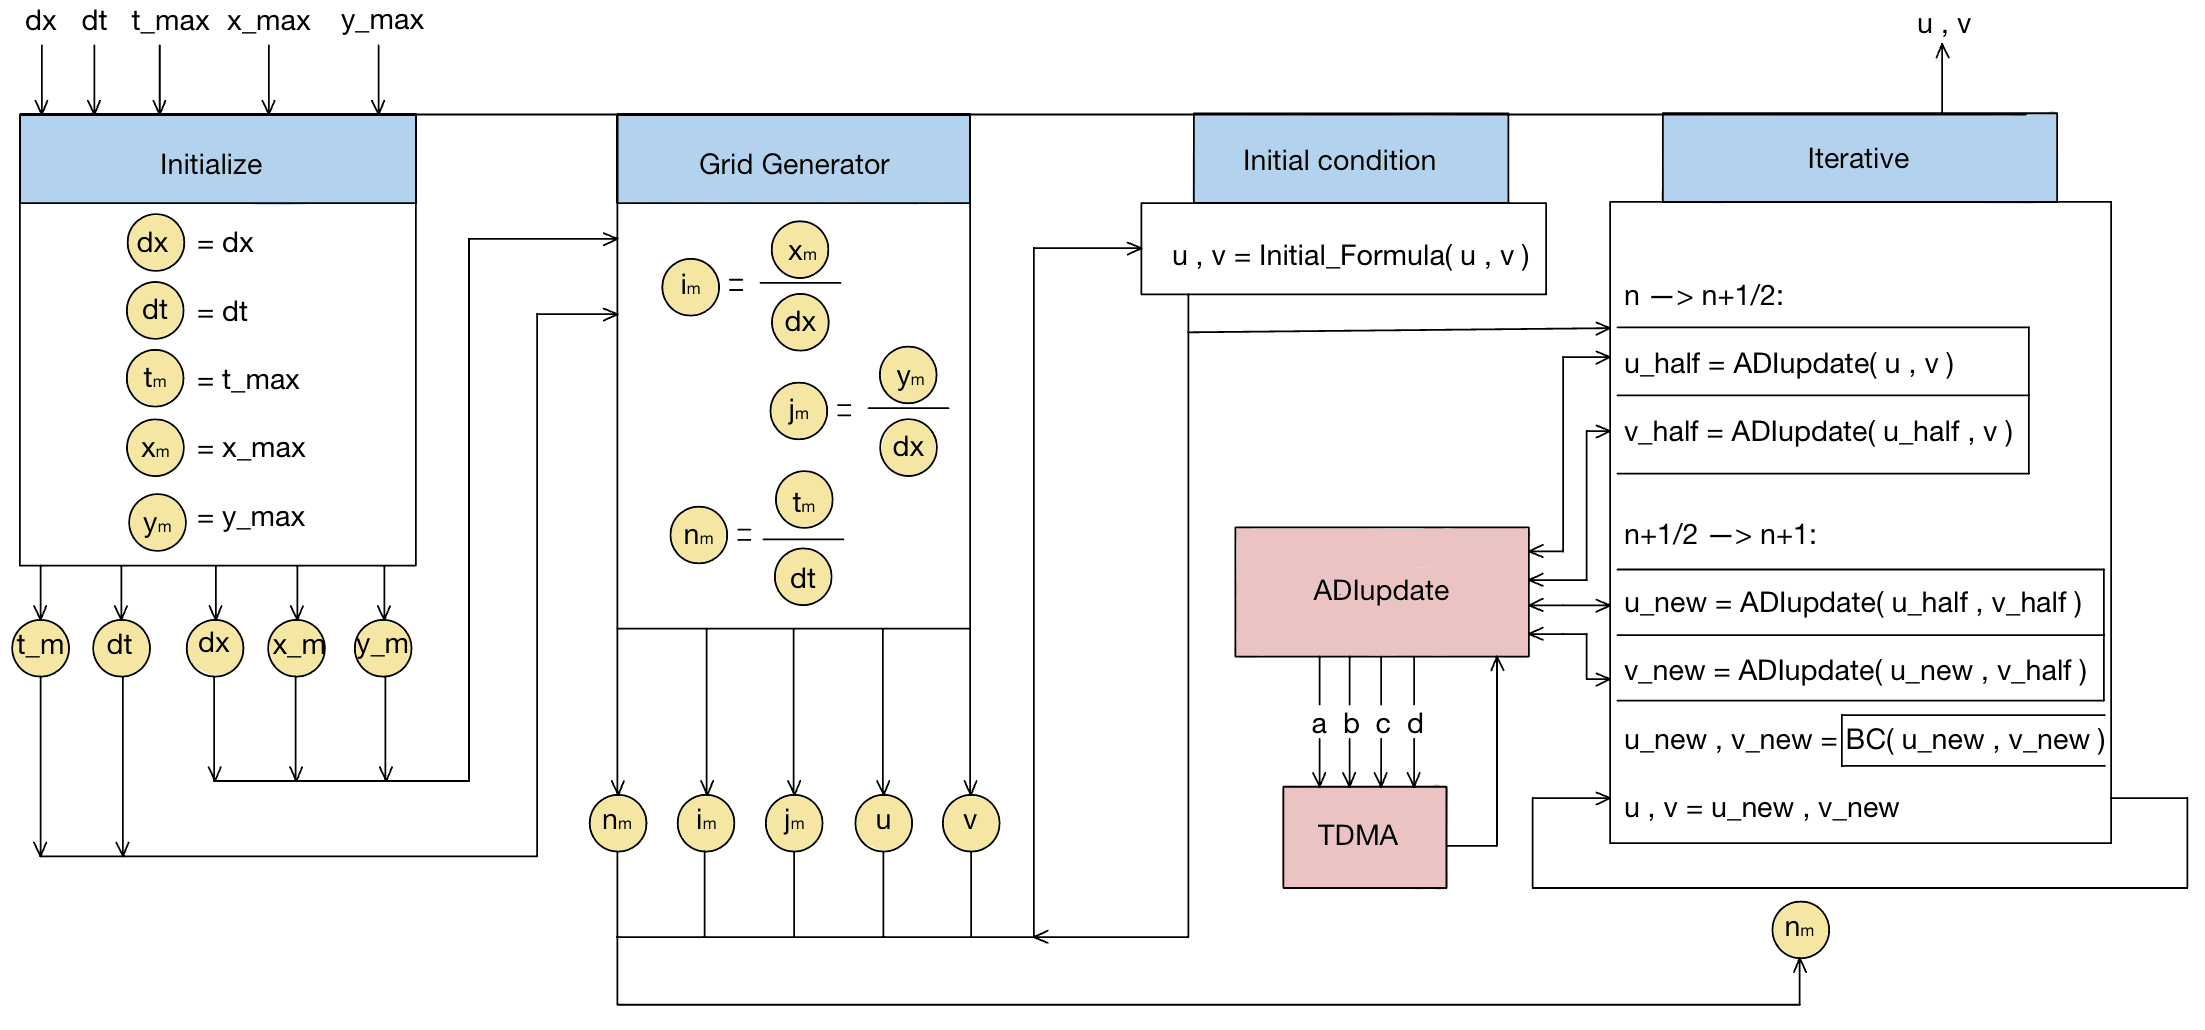
\includegraphics[width=1\textwidth]{figuresGeneral/Solver_Structure.jpg}
%     \label{IGs.jpg}
%     \caption{Solver Structure }
% \end{figure}

% % Algorithm:

% \begin{algorithm}[H]
%     \small
% \caption{xxx Method}
% \begin{algorithmic}[1]
% \For{ timestep = $n = 0$ to $N-1$} \Comment{Loop over time steps}
%     \State // Step from $n$ to $n+\frac{1}{2}$
%     \For{each each $j$ lines}  \Comment{Loop over each line}
%         \State a=b=c=($i_{max}$-1)x1 space, $a[i] = c[i] = a$, $b[i]  = b$
%         \State $U_{half}[i,j]$ = TDMA(a,b,c,d)
%     \EndFor
%     \State $U_{new}$ = BC($U_{new}$), $U = U_{new}$ 
% \EndFor

% \end{algorithmic}
% \end{algorithm}






%%%%%%%%%%%%%%%%%%%%%%%%%%%%%%%%%%%%%%%%%%%%%%%%%%%%%%%%%%%%%%%
%%%%%%%%%%%%%%%%%%%%%%%%%%%%%%%%%%%%%%%%%%%%%%%%%%%%%%%%%%%%%%%

\begin{document}

\title{\begin{Huge}Circular Cylinder Cross-Flow\end{Huge}\\530.767 CFD-Final Project\\Haobo Zhao}
\maketitle


This Project focuses on the CFD analysis of flow around circular and elliptical cylinders using a discretized Navier-Stokes (N-S) solver. This solver use $2^{nd}$ order central difference scheme in space and a second order (AB2 for convection and CN2 for viscous) fractional step in time. By separate update of the face velocity (“semi-staggered”  approach), we could approach zero divergence with the compact stencil for pressure. We also implemented Immersed Boundary Method (IBM) with stairs step method for inner boundary. We validated our solver based on uniform flow and channel flow, and compared our result with theordically solution. \\


We then simulated the flow cross circular cylinder at Re=150, checked our result against existing literature, ensuring soundness and reliability in our computational results. We also studied the influence of domain size, grid resolution, and Reynolds number on flow behavior was explored by modifying domain sizes from $8 \times 4$ to $8 \times 2$, adjusting grid resolutions from $\Delta =1/32$ and $\Delta = 1/16$, and analyzing results at Re = 300 and Re = 1000. Our findings indicate that for smaller domain sizes accelerate flow evolution and promote earlier vortex shedding due to enhanced fluid disturbances. Increasing the Reynolds number similarly affects flow susceptibility to disturbances. Conversely, a coarser grid resolution dampens disturbances, delaying vortex shedding but not preventing it, illustrating the fundamental role of grid resolution in fluid dynamics. 






\tableofcontents


\section{Question Review}

% Picture:
\begin{figure}[H]
    \centering
    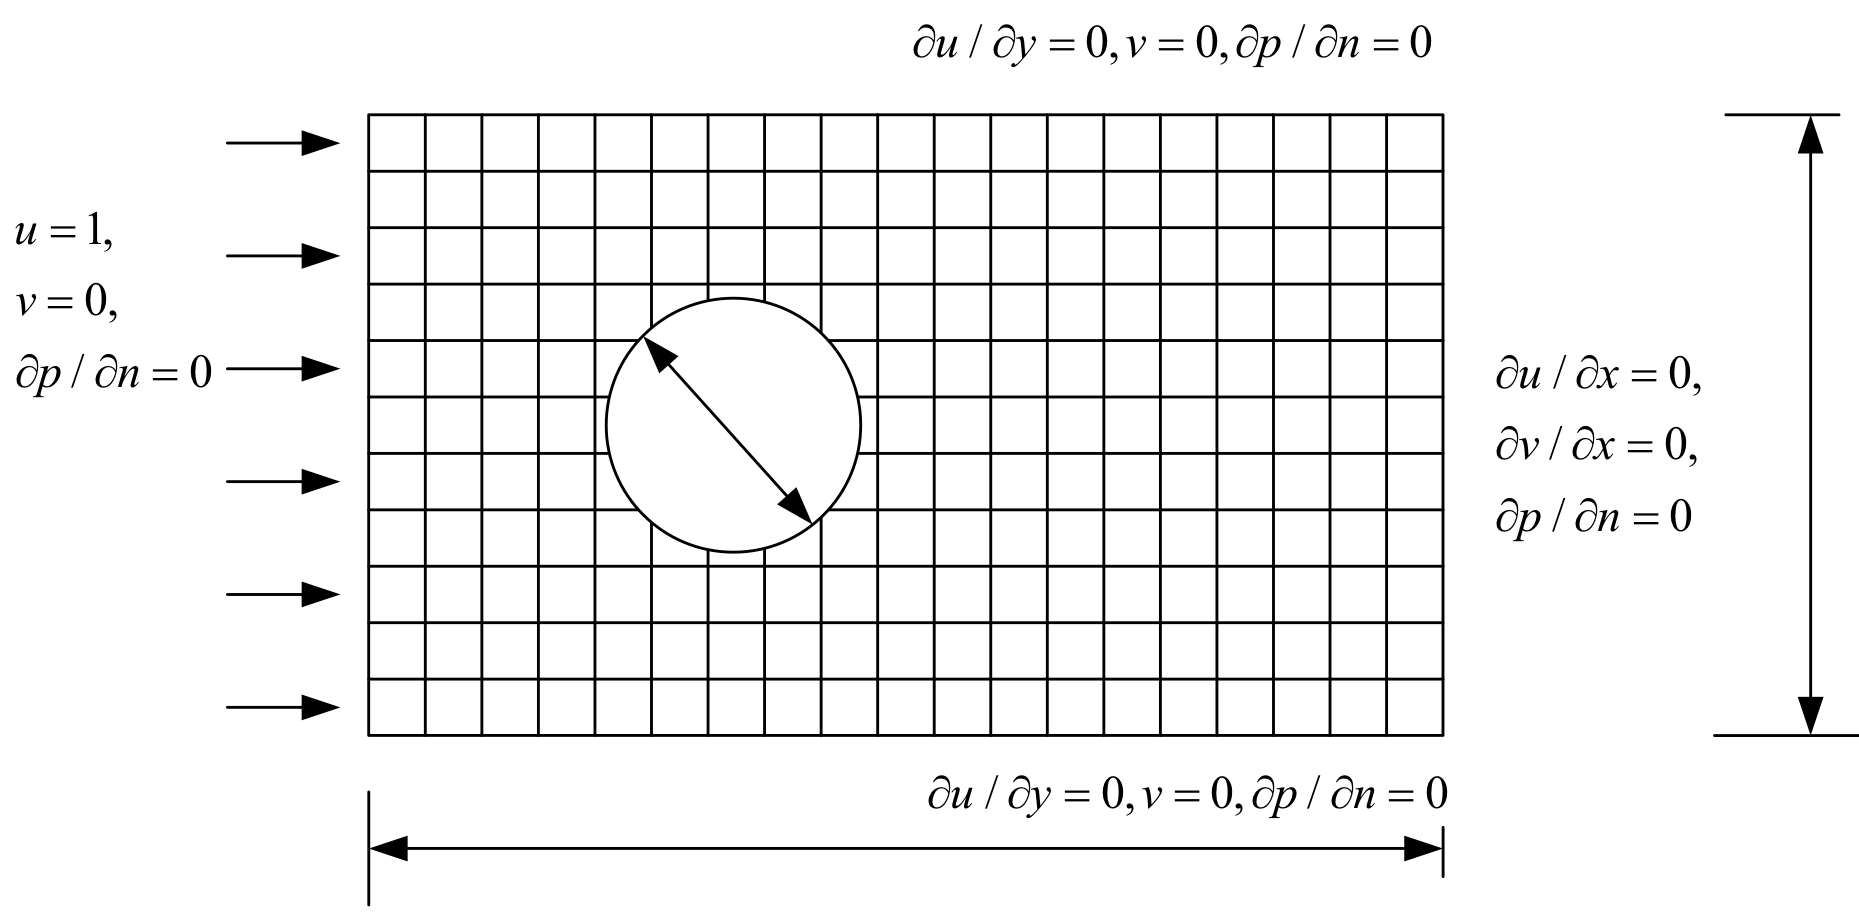
\includegraphics[width=1\textwidth]{figure/problem.jpg}
    \label{IGs.jpg}
\end{figure}



\subsection*{Circular cylinder in a cross-flow}
Consider a circular cylinder in a cross-flow as shown above.\\
The flow Reynolds number based on \(D\) is \(Re_D = 150\).

We will simulate this flow using:
\begin{itemize}
    \item Incompressible Navier-Stokes equations
    \item A Cartesian grid
    \item The Stair-Step, immersed boundary method.
    \item You can use either staggered or co-located (cell-centered) grid. If you use a co-located arrangement, then you should employ a separate face velocity update as shown in the class.
    \item A fractional-step method for time-stepping
    \item Use \(2^{nd}\) order central difference in space, and mixed implicit-explicit scheme in time.
    \item Domain size (\(L\) and \(H\)) shown in the figure is only suggestion. You can try different domain size.
    \item You can use either uniform or non-uniform grid. But non-uniform grid is recommended.
    \item At the outflow boundary, you will have to adjust the net flow in order to satisfy global mass conservation.
\end{itemize}

\subsection*{Tasks}
\begin{enumerate}
    \item[a)] Generate an appropriate computational grid and perform the flow simulation with the given boundary conditions but without the cylinder. Set the initial velocity inside the domain to zero. Check to make sure that your simulation converges well and you should see a uniform flow develop in your domain. The next sanity check is to impose a no-slip boundary conditions on the top and bottom walls in which case, you should see a flow similar to the flow in the entrance of a channel.
    
    \item[b)] Next, perform the simulation with the circular cylinder using the Stair-Step immersed boundary method. You should get unsteady flow exhibiting vortex shedding. If you don't get vortex shedding, try to improve your numerical schemes or grid resolution.
    
    \item[c)] Plot, velocity, pressure, and vorticity contours at several time instances.
    
    \item[d)] Quantify the vortex shedding frequency and compare the value against existing published studies.
    
    \item[e)] Quantify the pressure drag coefficient on the cylinder and compare the value against existing published studies.
    
    \item[f)] Examine the effect of domain size and grid resolution on the simulation results. Key quantities to be compared are the mean pressure drag coefficient and the shedding frequency.
    
    \item[g)] Simulate the same flow at \(Re_D = 300\) and \(1000\) and discuss the results in comparison to the \(Re_D = 150\) simulation. Do your results at higher Reynolds number match published results?
    
    \item[h)] Optional Extra credit – simulate the flow around a cylinder at a 3:1 elliptic cylinder with an angle-of-attack of 30 degrees, and a Reynolds number (based on major axis) of 300. Show that your code can predict the flow and vortex shedding from this shape. Plot the coefficient of pressure drag and lift versus Reynolds number.
\end{enumerate}




% \cite{GHIA1982387}
% \cite{BOTELLA1998421}


%%%%%%%%%%%%%%%%%%%%%%%%%%%%%%%%%%%%%%%%%%%%%%%%%%%%%%
%%%%%%%%%%%%%%%%%%%%%%%%%%%%%%%%%%%%%%%%%%%%%%%%%%%%%%
%%%%%%%%%%%%%%%%%%%%%%%%%%%%%%%%%%%%%%%%%%%%%%%%%%%%%%
%%%%%%%%%%%%%%%%%%%%%%%%%%%%%%%%%%%%%%%%%%%%%%%%%%%%%%

\newpage
\section{N-S Solver}
\subsection{Discretization of N-S Equation}
The general steps solving the N-S equation is showing below:

\begin{tabbing}
\hspace*{2cm} \= \hspace*{2.5cm} \= \kill
\textbf{(I):} \> Using the data from the current time step and the previous time step to get $u^{*}$, $v^{*}$. \\
\> Then use $u^{*}$, $v^{*}$ to get $U^{*}$, $V^{*}$.\\


\textbf{(II):} \> Using $U^{*}$, $V^{*}$, solving the pressure poisson equation (PPE),  get $p^{n+1}$.\\


\textbf{(III):} \> Using $p^{n+1}$, and $u^{*}$, $v^{*}$, get $u^{n+1}$, $v^{n+1}$. \\
\> Using $p^{n+1}$, and $U^{*}$, $V^{*}$, get $U^{n+1}$, $V^{n+1}$.
\end{tabbing}



\subsubsection{Step (I):}
Using the the data we got from current time step and the previous time step get $u^{*}$, $v^{*}$.
    Then use $u^{*}$, $v^{*}$ get $U^{*}$, $V^{*}$.



\noindent \textbf{Update $u^*, v^*$:}


The first step is going to update $u^*, v^*$:


\begin{equation}
    \frac{\vec{u}^{*} - \vec{u}^{n}}{\Delta t} = -[\frac{3}{2} \nabla \cdot (\vec{U}^n \vec{u}^{n}) - \frac{1}{2} \nabla \cdot (\vec{U}^{n-1} \vec{u}^{n-1}) ] + \frac{1}{Re} \nabla^{2} \frac{\vec{u}^*+\vec{u}^{n}}{2}
\end{equation}
    
which is:


    \begin{equation}
    \underbrace{[1 - \frac{\Delta t}{2Re}\nabla^2]\vec{u}^{*}}_{(1)} 
    = 
    -\frac{3}{2} \underbrace{[\Delta t \nabla \cdot (\vec{U}^n \vec{u}^{n})]}_{(2)} 
    + \frac{1}{2} \underbrace{[\Delta t  \nabla \cdot (\vec{U}^{n-1} \vec{u}^{n-1})]}_{(3)} 
    +\underbrace{[1+ \frac{\Delta t}{2Re} \nabla^{2}] \vec{u}}_{(4)}
\end{equation}

Could say, (2), (3) are convection term, and (4) is the diffusion term of the eqaution. 
Could use this equation to update $u^*$, $v^*$.


Where,
\begin{align*}
    (1) &= \left\{ 1 - \frac{\Delta t}{2Re} \nabla^2 \right\} u^{*} = P^{*} - \left[\frac{E^{*} + W^{*} - 2P^*}{\Delta x^{2}} + \frac{N^{*} + S^{*} - 2P^*}{\Delta y^{2}}\right] \frac{\Delta t}{2Re} \\
    (2) &= \frac{\Delta t}{\Delta} \left((U_{e}^{n} \frac{ E^{n} + P^{n}}{2} - U_{w}^{n} \frac{ W^{n} + P^{n}}{2}) + (V_{n}^{n} \frac{ N^{n} + P^{n}}{2} - V_{s}^{n} \frac{ S^{n} + P^{n}}{2}) \right) \\
    (3) &= \frac{\Delta t}{\Delta} \left((U_{e}^{n-1} \frac{ E^{n-1} + P^{n-1}}{2} - U_{w}^{n-1} \frac{ W^{n-1} + P^{n-1}}{2}) + (V_{n}^{n-1} \frac{ N^{n-1} + P^{n-1}}{2} - V_{s}^{n-1} \frac{ S^{n-1} + P^{n-1}}{2}) \right) \\
    (4) &= P^n + \frac{\Delta t}{2 Re \Delta^2} \left( E^{n} + W^{n} + N^{n} + S^{n} - 4P^{n} \right)
\end{align*}


    Could found in this expression, the formula to calculate $u^*$, $v^*$ is same, only input u or v in to the equation:

    $P$ means $(i,j)$, $W$ means $(i-1,j)$, $E$ means $(i+1,j)$, $S$ means $(i,j-1)$, $N$ means $(i,j+1)$.




\begin{figure}[H]
\centering
\begin{tikzpicture}[scale=1.5, every node/.style={scale=1}]
  % Draw grid
  \draw[step=1cm,black,thin] (1,1) grid (2,2);
  

  % Nodes for letters and coordinates
  \node at (0.5,1.5) {W};
  \node at (1.5,2.5) {N};
  \node at (1.5,1.5) {P};
  \node at (2.5,1.5) {E};
  \node at (1.5,0.5) {S};

  \node at (1,1.5) {w};
  \node at (1.5,1) {s};
  \node at (2,1.5) {e};
  \node at (1.5,2) {n};
  

  % Nodes for points
  \fill (0.5,1.5) circle[radius=0.2pt] node[below left] {$(j-1,j)$};
  \fill (1.5,2.5) circle[radius=0.2pt] node[above] {$(j,j+1)$};
  \fill (1.5,0.5) circle[radius=0.2pt] node[below] {$(j,j-1)$};
  \fill (2.5,1.5) circle[radius=0.2pt] node[below right] {$(j+1,j)$};

\end{tikzpicture}
\caption{Illustration of a grid layout with directional points.}
\end{figure}



Put the result in, could get:
$$
aW + bP + cE + eS + fN = d
$$


The left hand side is the unknown characters, and the right hand side b is known from previous and current time step. Could see, this equation in our system means $Ax = d$, where $A$ is consist of a,b,c,e,f, is a pentadiagonal matrix:


\[
\begin{bmatrix}
1 & 0 &   &   & 0 &   &    &\\
a & b & c &   &   & f &    &\\
  & a & b & c &   &   & f  &\\
  &   & a & b & c &   &    & 0\\
0 &   &   & \ddots & \ddots & \ddots &  &  \\
  & e &   &   & a & b & c &   &\\
  &   & e &   &   & a & b & c \\
  &   &   & 0 &   &   & 0 & 1 \\
\end{bmatrix}
\begin{bmatrix}
x_1 \\
x_2 \\
x_3 \\
x_4 \\
\vdots \\
x_{n-2} \\
x_{n-1} \\
x_n \\
\end{bmatrix}
=
\begin{bmatrix}
d_1 \\
d_2 \\
d_3 \\
d_4 \\
\vdots \\
d_{n-2} \\
d_{n-1} \\
d_{j\cdot i} \\
\end{bmatrix}
\]


Solve this system, we could get $u^*$, and $v^*$\\



\noindent \textbf{Update $U^*, V^*$:}\\
    $$ U_e^* = \frac{u_P^*+u_E^*}{2} , V_n^* = \frac{v_P^*+v_N^*}{2}$$


\subsubsection{Step (II):}
\textbf{Update $p^{n+1}$:}\\

$$
    \nabla^2 p = \frac{\nabla \cdot \vec{u}^*}{\Delta t}= \frac{\frac{U_e^* - U_w^*}{\Delta x} + \frac{V_n^* - V_s^*}{\Delta y}}{\Delta t}
$$

$$
\frac{P_E + P_W - 2P_P}{\Delta x^2} + \frac{P_N + P_S - 2P_P}{\Delta y^2} = \frac{\frac{U_e^* - U_w^*}{\Delta x} + \frac{V_n^* - V_s^*}{\Delta y}}{\Delta t}
$$

$$
P_E + P_W + P_N + P_S - 4P_P = \frac{\Delta}{\Delta t} \left( U_e^* - U_w^* + V_n^* - V_s^* \right) = RHS
$$

Similarly, this equation also give us a pentadiagonal system:


\[
\begin{bmatrix}
1 & 0 &   &   & 0 &   &    &\\
a & b & c &   &   & f &    &\\
  & a & b & c &   &   & f  &\\
  &   & a & b & c &   &    & 0\\
0 &   &   & \ddots & \ddots & \ddots &  &  \\
  & e &   &   & a & b & c &   &\\
  &   & e &   &   & a & b & c \\
  &   &   & 0 &   &   & 0 & 1 \\
\end{bmatrix}
\begin{bmatrix}
x_1 \\
x_2 \\
x_3 \\
x_4 \\
\vdots \\
x_{n-2} \\
x_{n-1} \\
x_n \\
\end{bmatrix}
=
\begin{bmatrix}
d_1 \\
d_2 \\
d_3 \\
d_4 \\
\vdots \\
d_{n-2} \\
d_{n-1} \\
d_n \\
\end{bmatrix}
\]





\subsubsection{Step (III):}
\textbf{Update $u^{n+1}$, $v^{n+1}$:}\\
The equation to update the $u^{n+1}$, $v^{n+1}$ is showing below:
$$
\vec{u}^{n+1} = \vec{u}^* - \Delta t (\nabla p)_{cc}
$$
where we could calculate the cell center pressure divergence $(\nabla p)_{cc}$, and:

$$
\begin{cases}
    u^{n+1} = u^* - \Delta t \cdot \frac{P_E - P_W}{2\Delta x} \\
    v^{n+1} = v^* - \Delta t \cdot \frac{P_N - P_S}{2\Delta y}
\end{cases}
$$


\noindent \textbf{Update $U^{n+1}$, $V^{n+1}$:}\\
The equation to update the $U^{n+1}$, $V^{n+1}$ is showing below:
$$
\vec{U}^{n+1} = \vec{U}^* - \Delta t (\nabla p)_{fc}
$$

where we could calculate the face center pressure divergence $(\nabla p)_{fc}$, and:


$$
\begin{cases}
    U_{e}^{n+1} = U_{e}^* - \Delta t \cdot \frac{P_E - P_P}{\Delta x} \\
    V_{n}^{n+1} = V_{n}^* - \Delta t \cdot \frac{P_N - P_P}{\Delta y}
    \end{cases}
$$

\subsubsection{LineSOR implementation}
In the discretization steps (I) and (II) of the Navier-Stokes equations, we obtain a pentadiagonal matrix system. However, our Tridiagonal Matrix Algorithm (TDMA) can only solve systems represented by tridiagonal matrices. To address this, we transfer the additional diagonal lines, e and f, to the right-hand side and continue iterating. This process is repeated until the results satisfy the original requirements of the pentadiagonal system.\\



\noindent \textbf{The origional pentadiagonal system:}

\[
\begin{bmatrix}
1 & 0 &   &   & 0 &   &    &\\
a & b & c &   &   & f &    &\\
  & a & b & c &   &   & f  &\\
  &   & a & b & c &   &    & 0\\
0 &   &   & \ddots & \ddots & \ddots &  &  \\
  & e &   &   & a & b & c &   &\\
  &   & e &   &   & a & b & c \\
  &   &   & 0 &   &   & 0 & 1 \\
\end{bmatrix}
\begin{bmatrix}
u_1 \\
u_2 \\
u_3 \\
u_4 \\
\vdots \\
u_{n-2} \\
u_{n-1} \\
u_n \\
\end{bmatrix}
=
\begin{bmatrix}
d_1 \\
d_2 \\
d_3 \\
d_4 \\
\vdots \\
d_{n-2} \\
d_{n-1} \\
d_n \\
\end{bmatrix}
\]




For each line j, the system could be represented as:

\[
\left[
\begin{array}{c|c|c}
E & T & F 
\end{array}
\right]
\begin{bmatrix}
    [u_{j-1}^{n+1}] \\
    [u_{j}^{n+1}] \\
   [ u_{j+1}^{n+1}]
\end{bmatrix}
=
\begin{bmatrix}
    [d_{j}] \\
\end{bmatrix}
\]

Could say, E mans operating the previous line (j-1) to current line (j), and F means operating on the next line (j+1) to current line. Where $\left[
\begin{array}{c|c|c}
E & T & F 
\end{array}
\right]$ is:


\[
\left[
\begin{array}{cccccc|cccccc|cccccc}
0 & 0 & \cdots & 0 & 0 & 0 & 1 & 0 & 0 & \cdots & 0 & 0 & 0 & 0 & \cdots & 0 & 0 & 0 \\
0 & e_{2} & 0 & \cdots & 0 & 0 & a_{2} & b_{2} & c_{2} & \ddots & \vdots & 0 & 0 & f_{2} & 0 & \cdots & 0 & 0 \\
0 & 0 & e_{3} & \cdots & 0 & 0 & 0 & a_{3} & \ddots & \ddots & 0 & 0 & 0 & 0 & f_{3} & \cdots & 0 & 0 \\
0 & \vdots & \vdots & \ddots & \vdots & \vdots & \vdots & \ddots & \ddots & \ddots & c_{2} & 0 & 0 & \vdots & \vdots & \ddots & \vdots & \vdots \\
0 & 0 & 0 & \cdots & e_{n-1} & 0 & 0 & \ddots & \ddots & 0 & b_{n-1} & c_{n-1} & 0 & 0 & 0 & \cdots & f_{n-1} & 0 \\
0 & 0 & 0 & \cdots & 0 & 0 & 0 & \cdots & 0 & 0 & 0 & 1 & 0 & 0 & 0 & \cdots & 0 & 0 \\
\end{array}
\right]
\]\\

\textbf{LineSOR:}\\

For LineSOR, we move the two diagonal line (e and f) to the right hand side:

\[
\left[
\begin{array}{c|c|c}
0 & T & 0 
\end{array}
\right]
\begin{bmatrix}
    [u_{j-1}^{k+1}] \\
    [u_{j}^{k+1}] \\
   [ u_{j+1}^{k+1}]
\end{bmatrix}
=
\begin{bmatrix}
    [d_{j}] \\
\end{bmatrix}
-
\left[
\begin{array}{c|c|c}
E & 0 & F 
\end{array}
\right]
\begin{bmatrix}
    [u_{j-1}^{k}] \\
    [u_{j}^{k}] \\
   [ u_{j+1}^{k}]
\end{bmatrix}
\]


Which is:

\[
\left[
T
\right]
\begin{bmatrix}
    [u_{j}^{k+1}]
\end{bmatrix}
=
\begin{bmatrix}
    [d_{j}] \\
\end{bmatrix}
-
\left[
E
\right]
\begin{bmatrix}
    [u_{j-1}^{k}]
\end{bmatrix}
-
\left[
F
\right]
\begin{bmatrix}
    [u_{j+1}^{k}]
\end{bmatrix}
\]







Where we could use TDMA to solve this equation. As this result is different from directly solve the equation we previously got, we need it keep iterating, until the error small enough:


\[ 
Error = 
\left[
\begin{array}{c|c|c}
E & T & F 
\end{array}
\right]
\begin{bmatrix}
    [u_{j-1}^{k+1}] \\
    [u_{j}^{k+1}] \\
   [ u_{j+1}^{k+1}]
\end{bmatrix}
-
\begin{bmatrix}
    [d_{j}] \\
\end{bmatrix}
<1e-6
\]


%%%%%%%%%%%%%%%%%%%%%%%%%%%%%%%%%%%%%%%%%%%%%%%%%%%%%%

\subsection{Immersed Boundary Method}
\subsubsection{Coefficient Correction}



\noindent As our original Governing Equation as follows:
$$
c_W f_W + c_S f_S + c_P f_P + c_N f_N + c_E f_E = \text{RHS}
$$

Lets first consider the East point of our control point is solid point, which in two different kind of boundary condition is: 


\begin{itemize}
    \item  Dirichlet condition: $f = f_F$ \item Neumann condition: $\frac{\partial f}{\partial n} = f_p$
\end{itemize}

\begin{figure}[H]
\centering
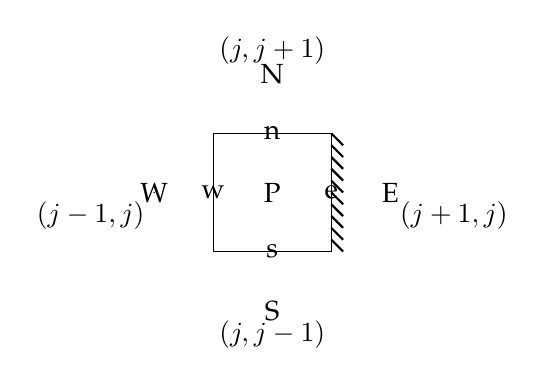
\begin{tikzpicture}[scale=1.5, every node/.style={scale=1}]
  % Draw grid
  \draw[step=1cm,black,thin] (1,1) grid (2,2);
  

  % Nodes for letters and coordinates
  \node at (0.5,1.5) {W};
  \node at (1.5,2.5) {N};
  \node at (1.5,1.5) {P};
  \node at (2.5,1.5) {E};
  \node at (1.5,0.5) {S};

  \node at (1,1.5) {w};
  \node at (1.5,1) {s};
  \node at (2,1.5) {e};
  \node at (1.5,2) {n};
  

  % Nodes for points
  \fill (0.5,1.5) circle[radius=0.2pt] node[below left] {$(j-1,j)$};
  \fill (1.5,2.5) circle[radius=0.2pt] node[above] {$(j,j+1)$};
  \fill (1.5,0.5) circle[radius=0.2pt] node[below] {$(j,j-1)$};
  \fill (2.5,1.5) circle[radius=0.2pt] node[below right] {$(j+1,j)$};

  % Draw the lines
    \foreach \x in {1.1,1.2,1.3,1.4,1.5,1.6,1.7,1.8,1.9,2}{
        \draw[thick] (2,\x) -- (2.1,\x-0.1);
    }

\end{tikzpicture}
\caption{Illustration of a grid layout with directional points.}
\end{figure}




\noindent \textbf{Dirichlet condition} 

\noindent For boundary at East:

\[
c_W f_W + c_S f_S + c_P f_P + c_N f_N + c_E\underbrace{ f_E}_{2E-f_P} = \text{RHS}
\]




Where, E is the value at the east boundary. The equation then becomes:

\[
\underbrace{c_W f_W + c_S f_S+ c_N f_N}_{(1)}  + \underbrace{(c_P - c_E) f_P }_{(2)}
= 
\text{RHS} - 2E
\]

\noindent For different boundary location:
$$
(1) = iF_W \cdot c_W f_W + iF_S \cdot c_S f_S + iF_N \cdot c_N f_N + iF_E \cdot c_E f_E
$$
$$
(2) = \left[ c_P - ((1-iF_E) c_E + (1-iF_S) c_S + (1-iF_N) c_N (1-iF_W) c_W) \right] f_P
$$

Where $iF$ is the field (array) have same shape with u, but only contains 0 (for solid point) or 1 (for fluid point) on each point, to determine whether the point is in fluid.\\


\noindent As the value at our inner boundary are 0,
the equation then becomes:
$$
(1) + (2) = RHS
$$






\noindent \textbf{Neumann  condition} 

\noindent For boundary at East:

Similar, our inner boundary is 0-gradient,
\[
c_W f_W + c_S f_S + c_P f_P + c_N f_N + c_E\underbrace{ f_E}_{f_P} = \text{RHS}
\]


Where, E is the value at the east boundary. The equation then becomes:

\[
\underbrace{c_W f_W + c_S f_S+ c_N f_N}_{(1)}  + \underbrace{(c_P + c_E) f_P }_{(2)}
= 
\text{RHS} 
\]

\noindent For different boundary location:
$$
(1) = iF_W \cdot c_W f_W + iF_S \cdot c_S f_S + iF_N \cdot c_N f_N + iF_E \cdot c_E f_E
$$
$$
(2) = \left[ c_P + ((1-iF_E) c_E + (1-iF_S) c_S + (1-iF_N) c_N (1-iF_W) c_W) \right] f_P
$$



\noindent The equation then becomes:
$$
(1) + (2) = RHS
$$



\noindent Thus, change coefficients for N,S,E,W points is showing below::
\[
c_W = iF_W \cdot c_W
\]
\[
c_S = iF_S \cdot c_S
\]
\[
c_N = iF_N \cdot c_N
\]
\[
c_E = iF_E \cdot c_E
\]

The $C_P$ for Dirichlet condition is showing below:

\[
c_P = c_P - ((1-iF_E) c_E + (1-iF_S) c_S + (1-iF_N) c_N (1-iF_W) c_W)
\]

\noindent The change coefficients for Neumann:
\[
c_P = c_P + ((1-iF_E) c_E + (1-iF_S) c_S + (1-iF_N) c_N (1-iF_W) c_W)
\]

Finally, we need to make sure for solid points, our equation could work:

\[
c_P = c_P \cdot iF + iS, \vspace{15pt} RHS = RHS \cdot iF
\]

Where, $iF$ is the field only contains 1 at fluid points, 0 for solid points. $iS$, on the contrary, only contains 1 at solid points, but 0 for fluid points. 





\subsection{Solver field Setting}
As in the discretization of N-S equation, we have $u$, $v$, $p$, and $U$, $V$ fields. To handle boundary condition, we use ghost point. For convenient, we set all the fields in same size: $(N+2) \cdot (N+2)$, the u, v, p fields are:

\begin{figure}[H]
    \centering
    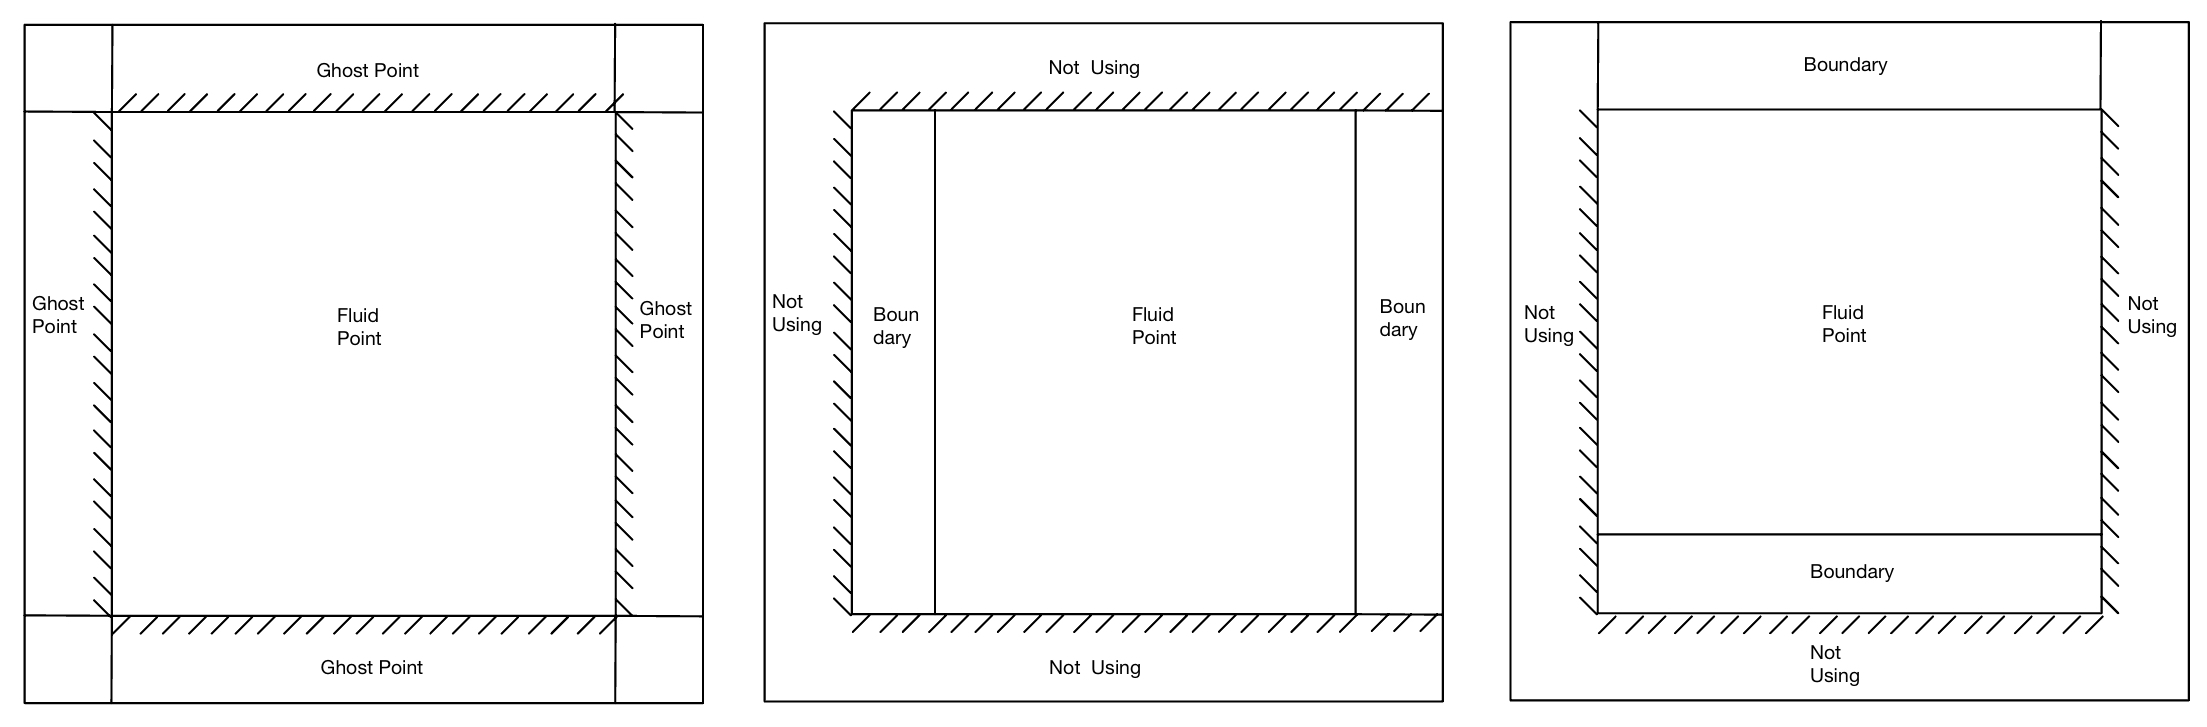
\includegraphics[width=0.9\linewidth]{figure/Domain.jpg}
    \caption{u/v/p, U, and V field}
\end{figure}

The left one is for u, v, and p field, where they are defined at cell center. It contains ghost point, which is in the solid part near to the boundary. U field is in the middle, which is 1 column, and 2 rows less than u/v/p field. V field is the right one, where it is 1 row, and 2 column less than u/v/p field.


% \begin{figure}[H]
% \centering
% \begin{tikzpicture}[scale=2, every node/.style={scale=1}]
%   % Draw grid
%   \draw[step=1cm,black,thin] (0,0) grid (3,3);
  

%   % Nodes for letters and coordinates
%   \node at (0.5,1.5) {$u_{i-1,j}$};
%   \node at (1.5,2.5) {$u_{i,j+1}$};
%   \node at (1.5,1.5) {$u_{i,j}$};
%   \node at (2.5,1.5) {$u_{i+1,j}$};
%   \node at (1.5,0.5) {$u_{i,j-1}$};

%   \node at (1,1.5) {$U_{i,j}$};
%   \node at (1.5,1) {$V_{i,j}$};
%   \node at (2,1.5) {$U_{i+1,j}$};
%   \node at (1.5,2) {$V_{i,j+1}$};
  
% \end{tikzpicture}
% \caption{Illustration of a grid layout with u/v/p, U, and V.}
% \end{figure}






\subsection{Solver Architecture}
\begin{figure}[H]
    \centering
    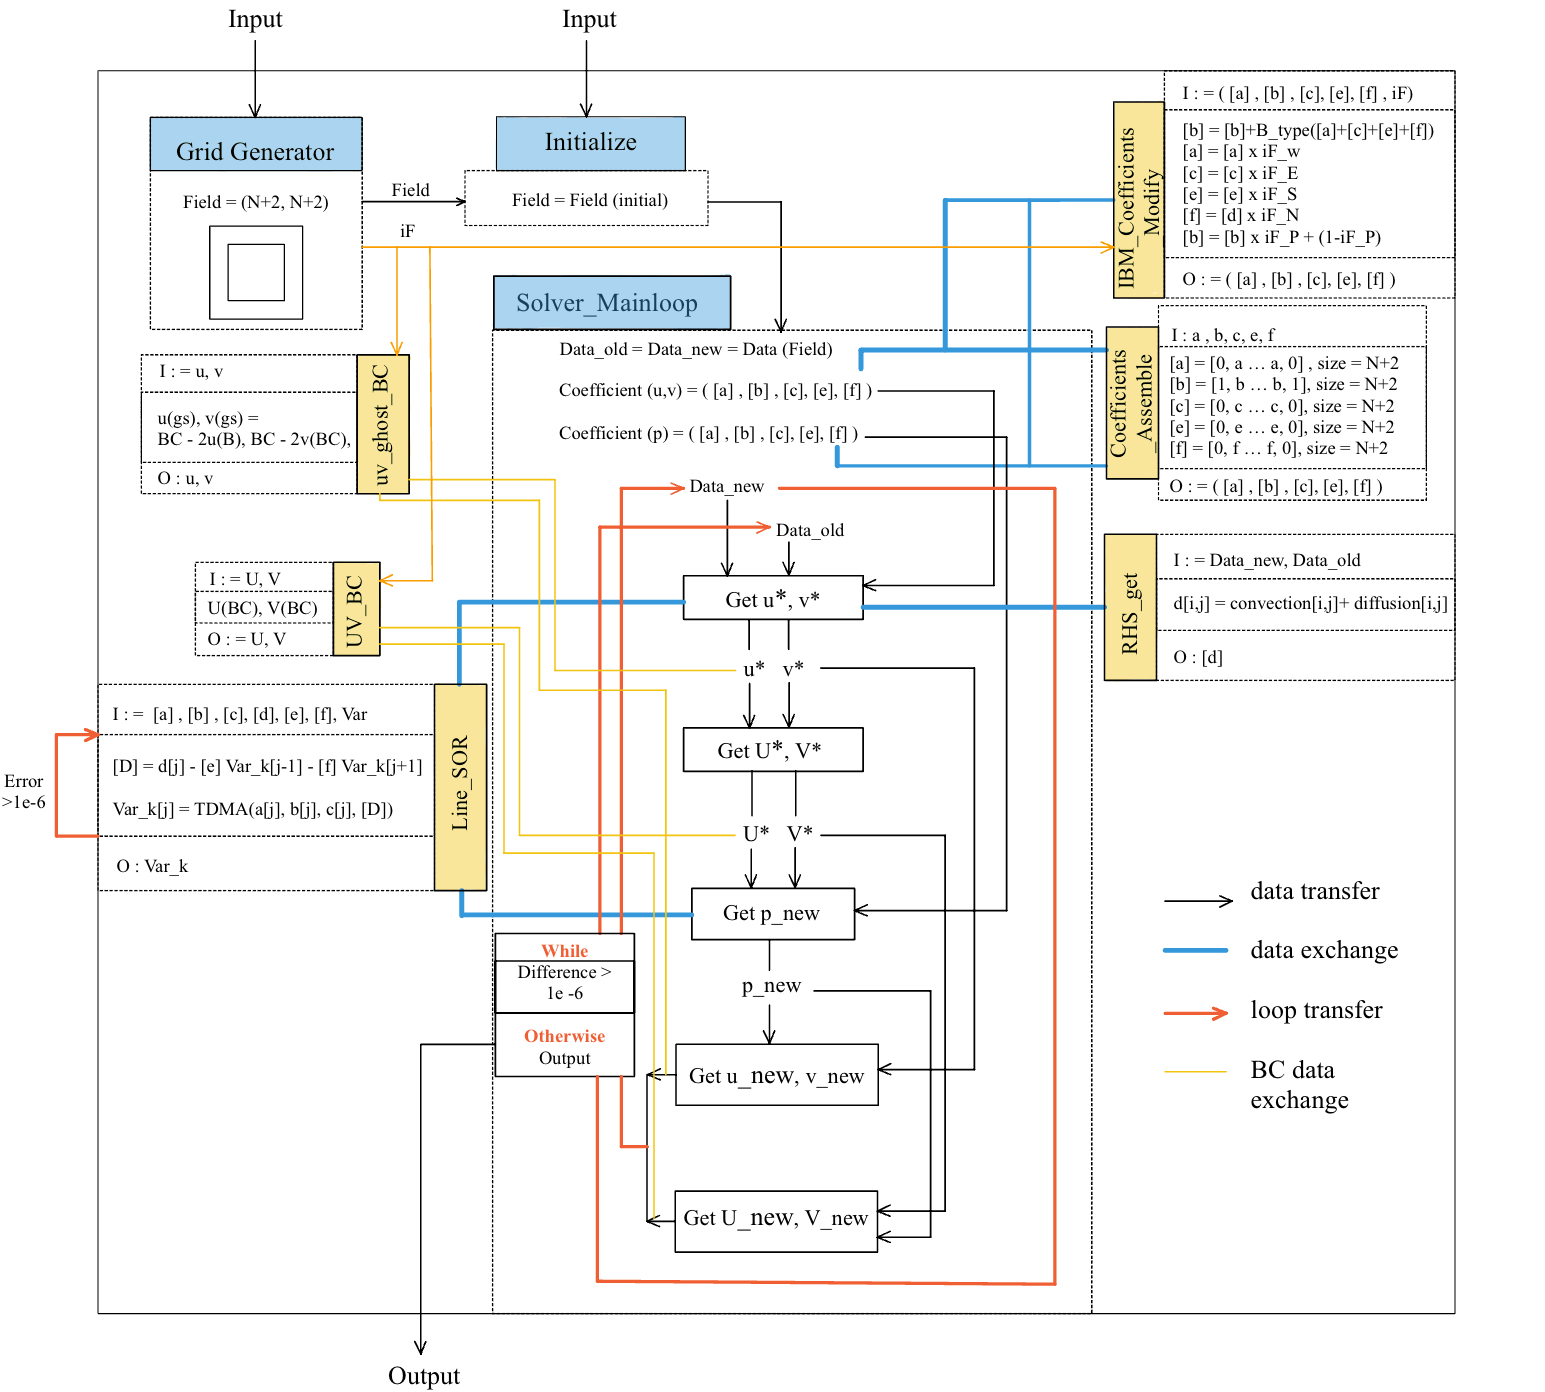
\includegraphics[width=1\linewidth]{figure/Solver and Stting/Solver_Strture.jpg}
    \caption{Solver Architecture}
\end{figure}


This diagram shows our Solver structure. By Using grid generator to generate fields for $u, v, p$, and $U, V$, transfer the data to initialize the initial value, then use the main loop to doing time iteration till the fields get to steady state, we could output the result. \\

\begin{itemize}
    \item \textbf{I/O}: I means function input, and O means function output.
    \item \textbf{Data Transfer Lines}: The diagram uses different colored lines to indicate various types of data movement, while the lines with arrow means one-way data transfer, which means value assignment, and the lines without arrow means data exchange, where there is data input to function, but there is also data get back from function.
\end{itemize}
































\newpage
\section{Solver Testing--Uniform and Channel Case}
\subsection{Uniform flow}

We used the same boundary condition as the requirement shown before but without the cylinder. The simulation converges, and the uniform flow developed has been observed:

\begin{figure}[H]
    \centering
    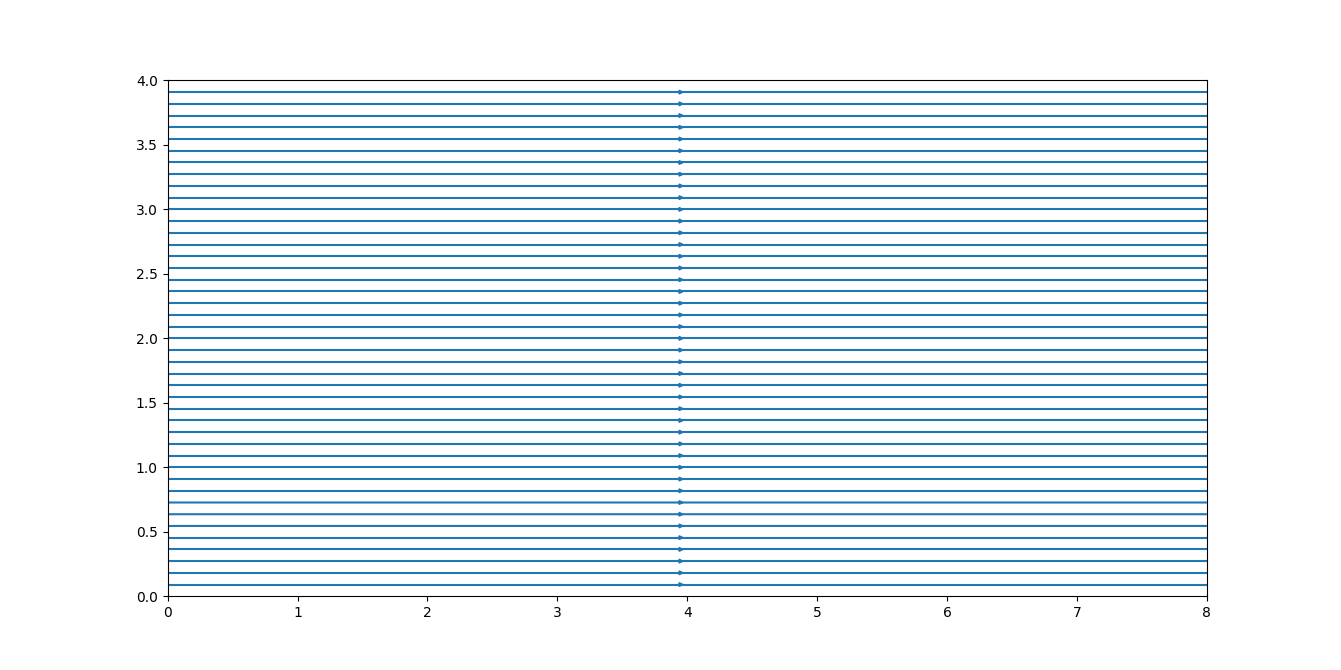
\includegraphics[width=0.6\linewidth]{figure/Uniformflow.jpg}
    \caption{Streamline of the result}
\end{figure}









\subsection{Channel Flow}
\subsubsection{Flow setting}
We setup channel flow case for test our N-S solver is working well, where the setting is showing below:

\begin{figure}[H]
    \centering
    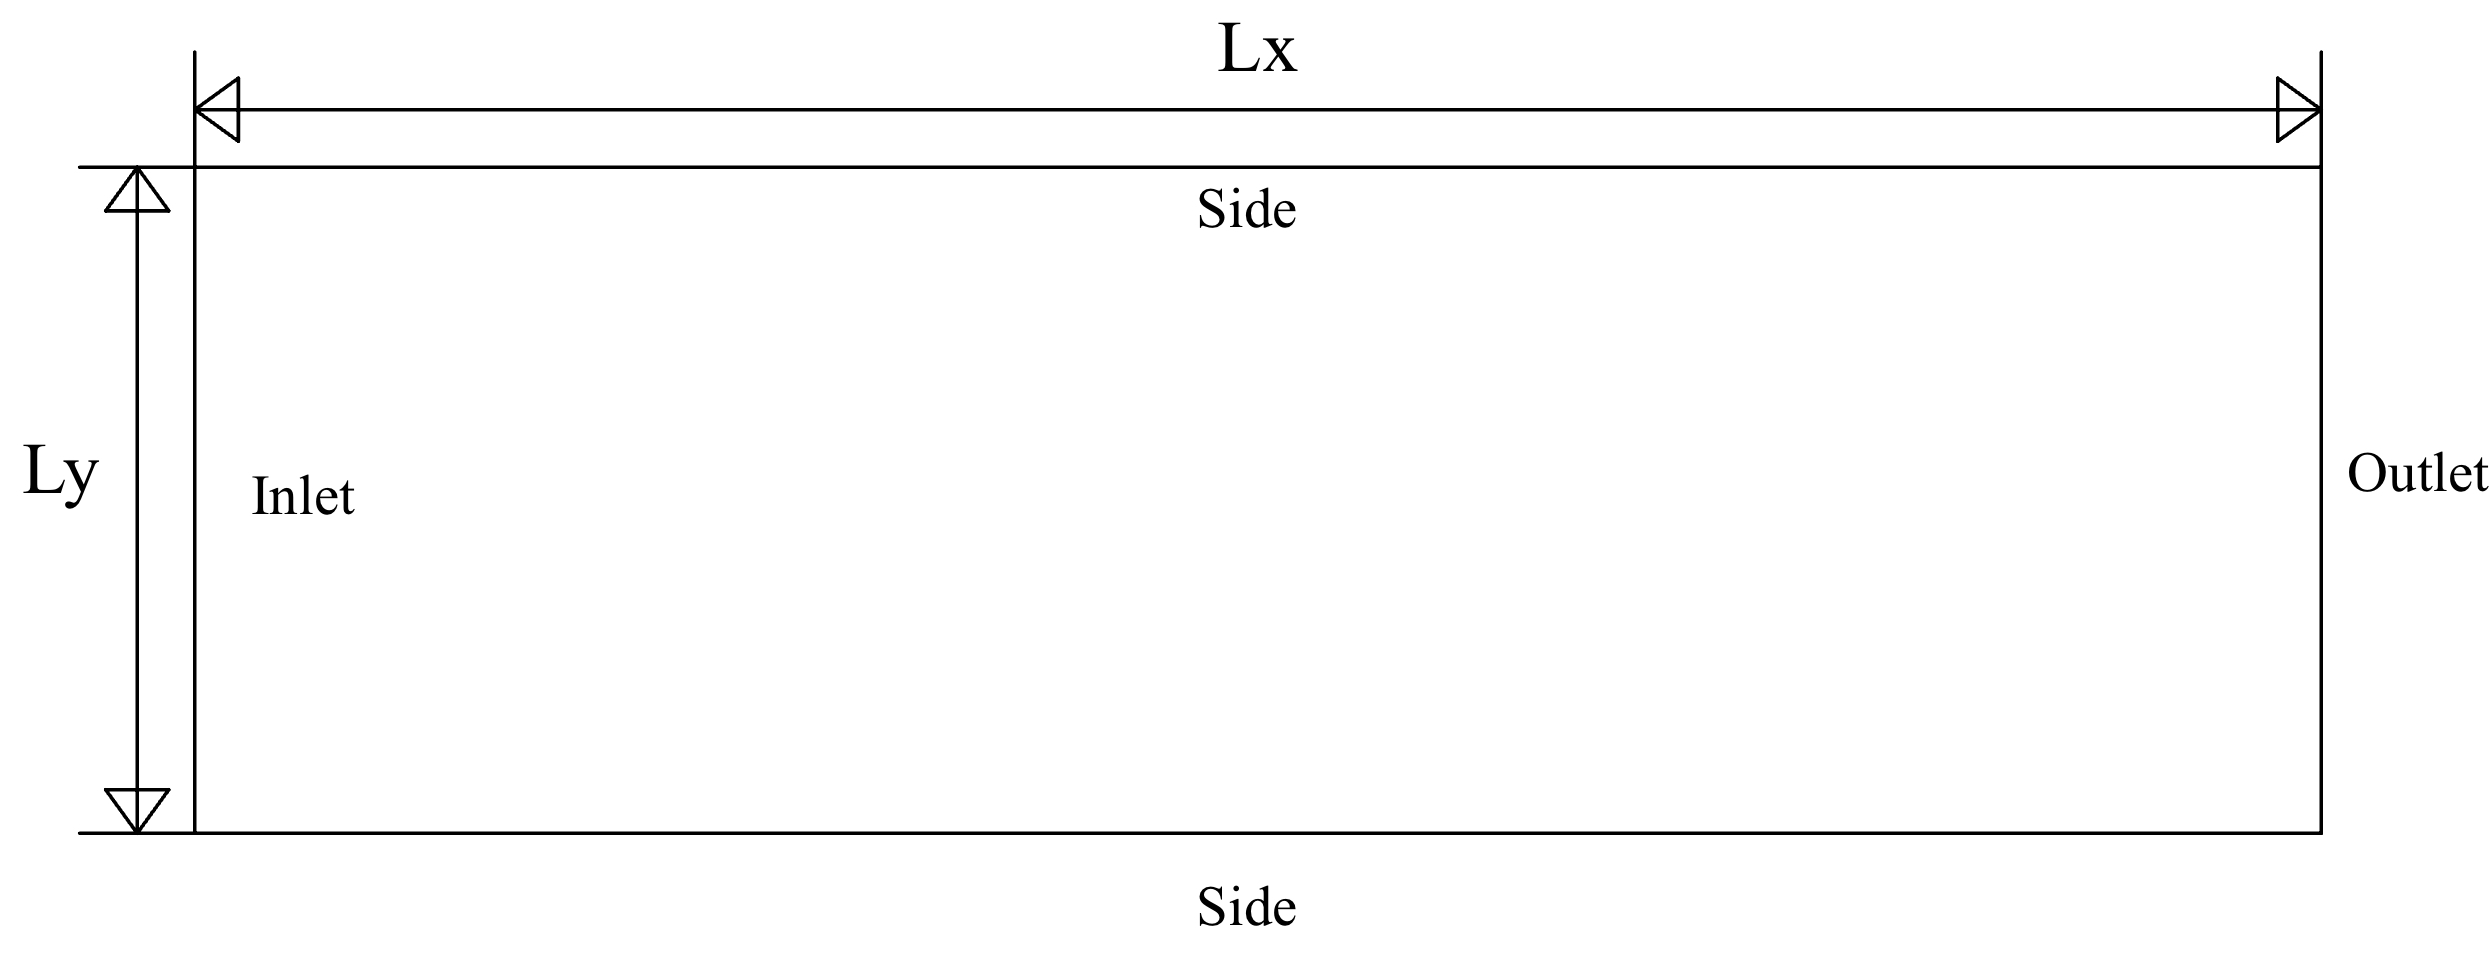
\includegraphics[width=0.6\linewidth]{figure/Solver and Stting/Channel_Setting.jpg}
    \caption{Domain and boundary setting for Channel flow}
\end{figure}

The Domain setting as shown above. The key parameters as follows:
\begin{itemize}
    \item \textbf{Ly=1, Lx=10}: Width and Length of the domain
    \item \textbf{Inlet}: $u=1, v=0, \frac{\partial p}{\partial x}=0$
    \item \textbf{Side}: $u=v=0, \frac{\partial p}{\partial y}=0$
    \item \textbf{Outlet}: $\frac{\partial u}{\partial x}=0, v=0, 
    \frac{\partial p}{\partial x}=0$
\end{itemize}


\subsubsection{Result}
The result is showing below:
\begin{figure}[H]
    \centering
    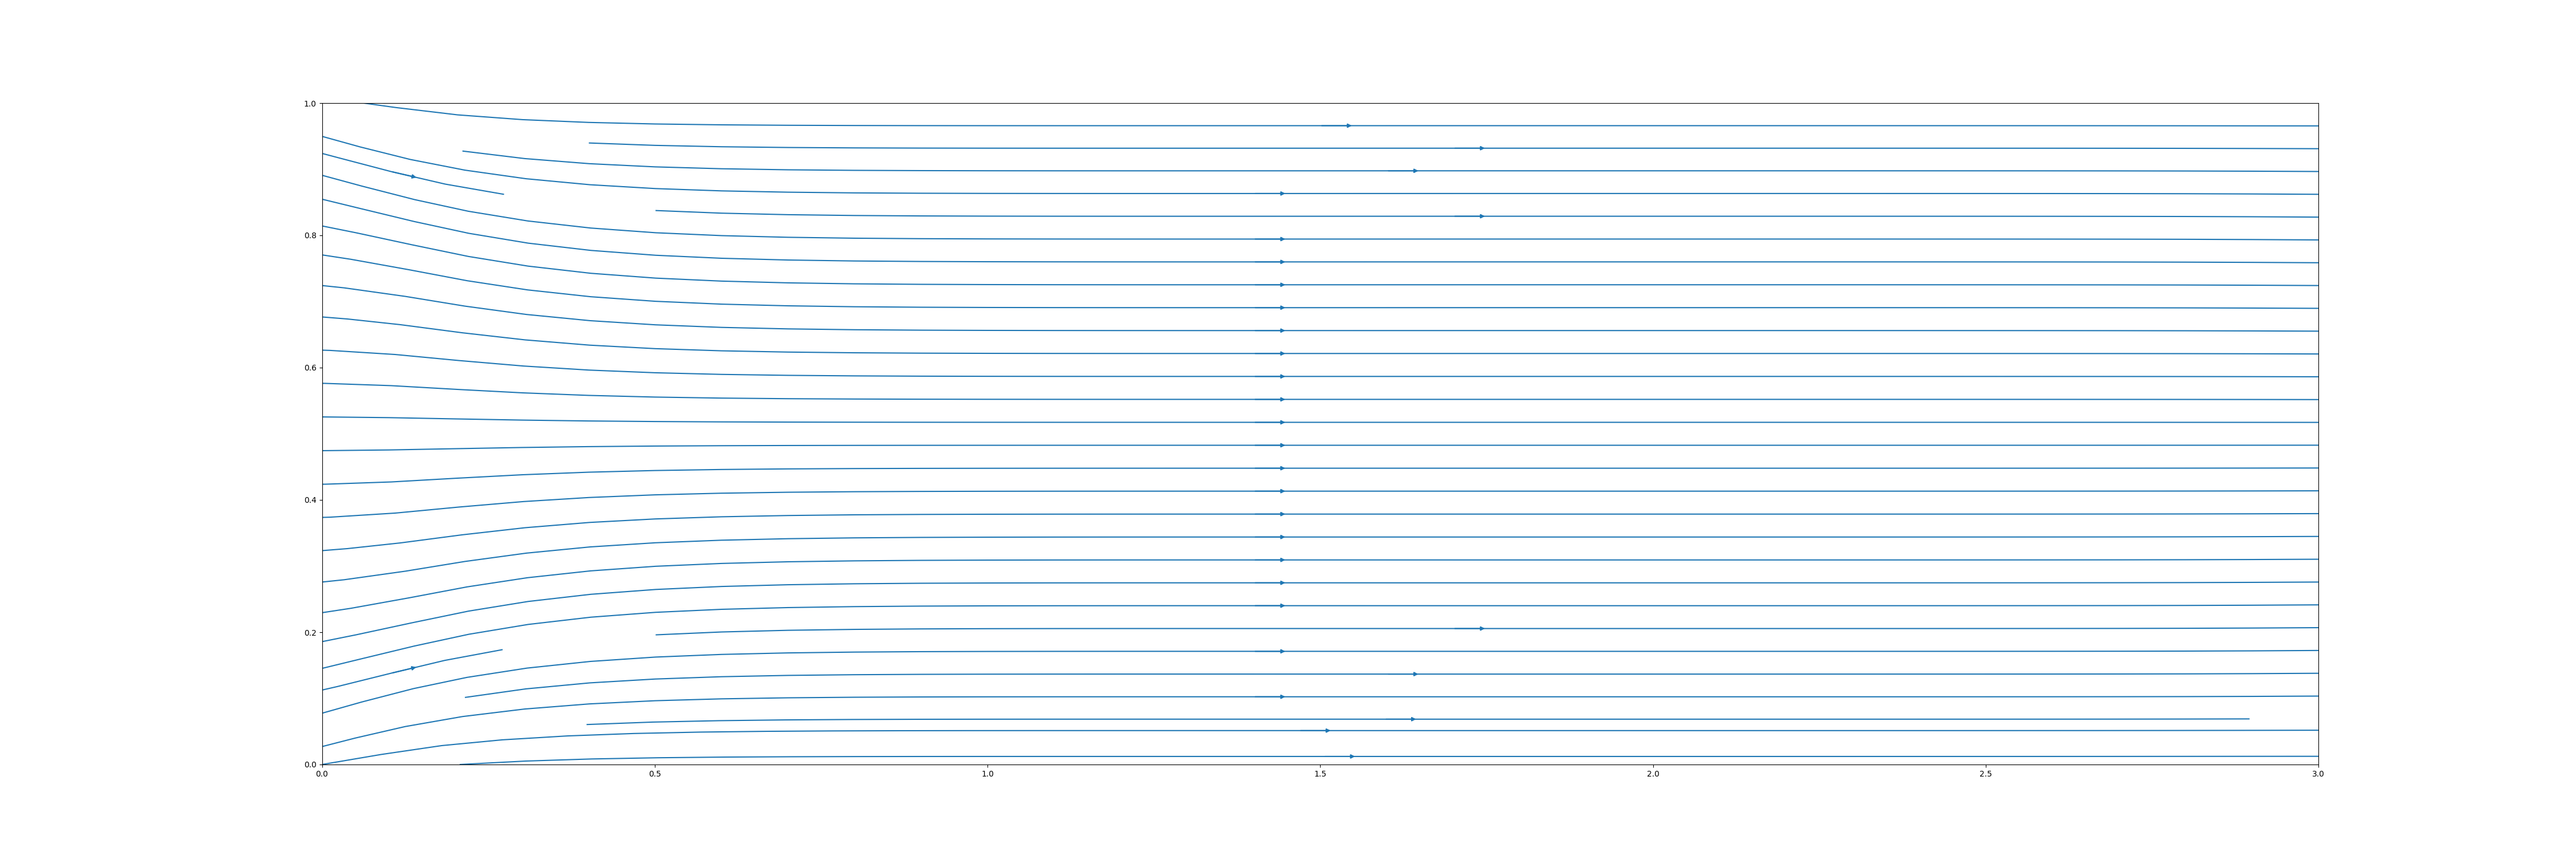
\includegraphics[width=1\linewidth]{figure/Channel_flow/cyl_stline_N=96, Re=10.0, t=50.0.jpg}
    \caption{Streamline at t=50s}
\end{figure}

This diagram shows the streamline at t=50s, where we could see there the flow do follow our boundary condition and developed as expected.

\begin{figure}[H]
    \centering
    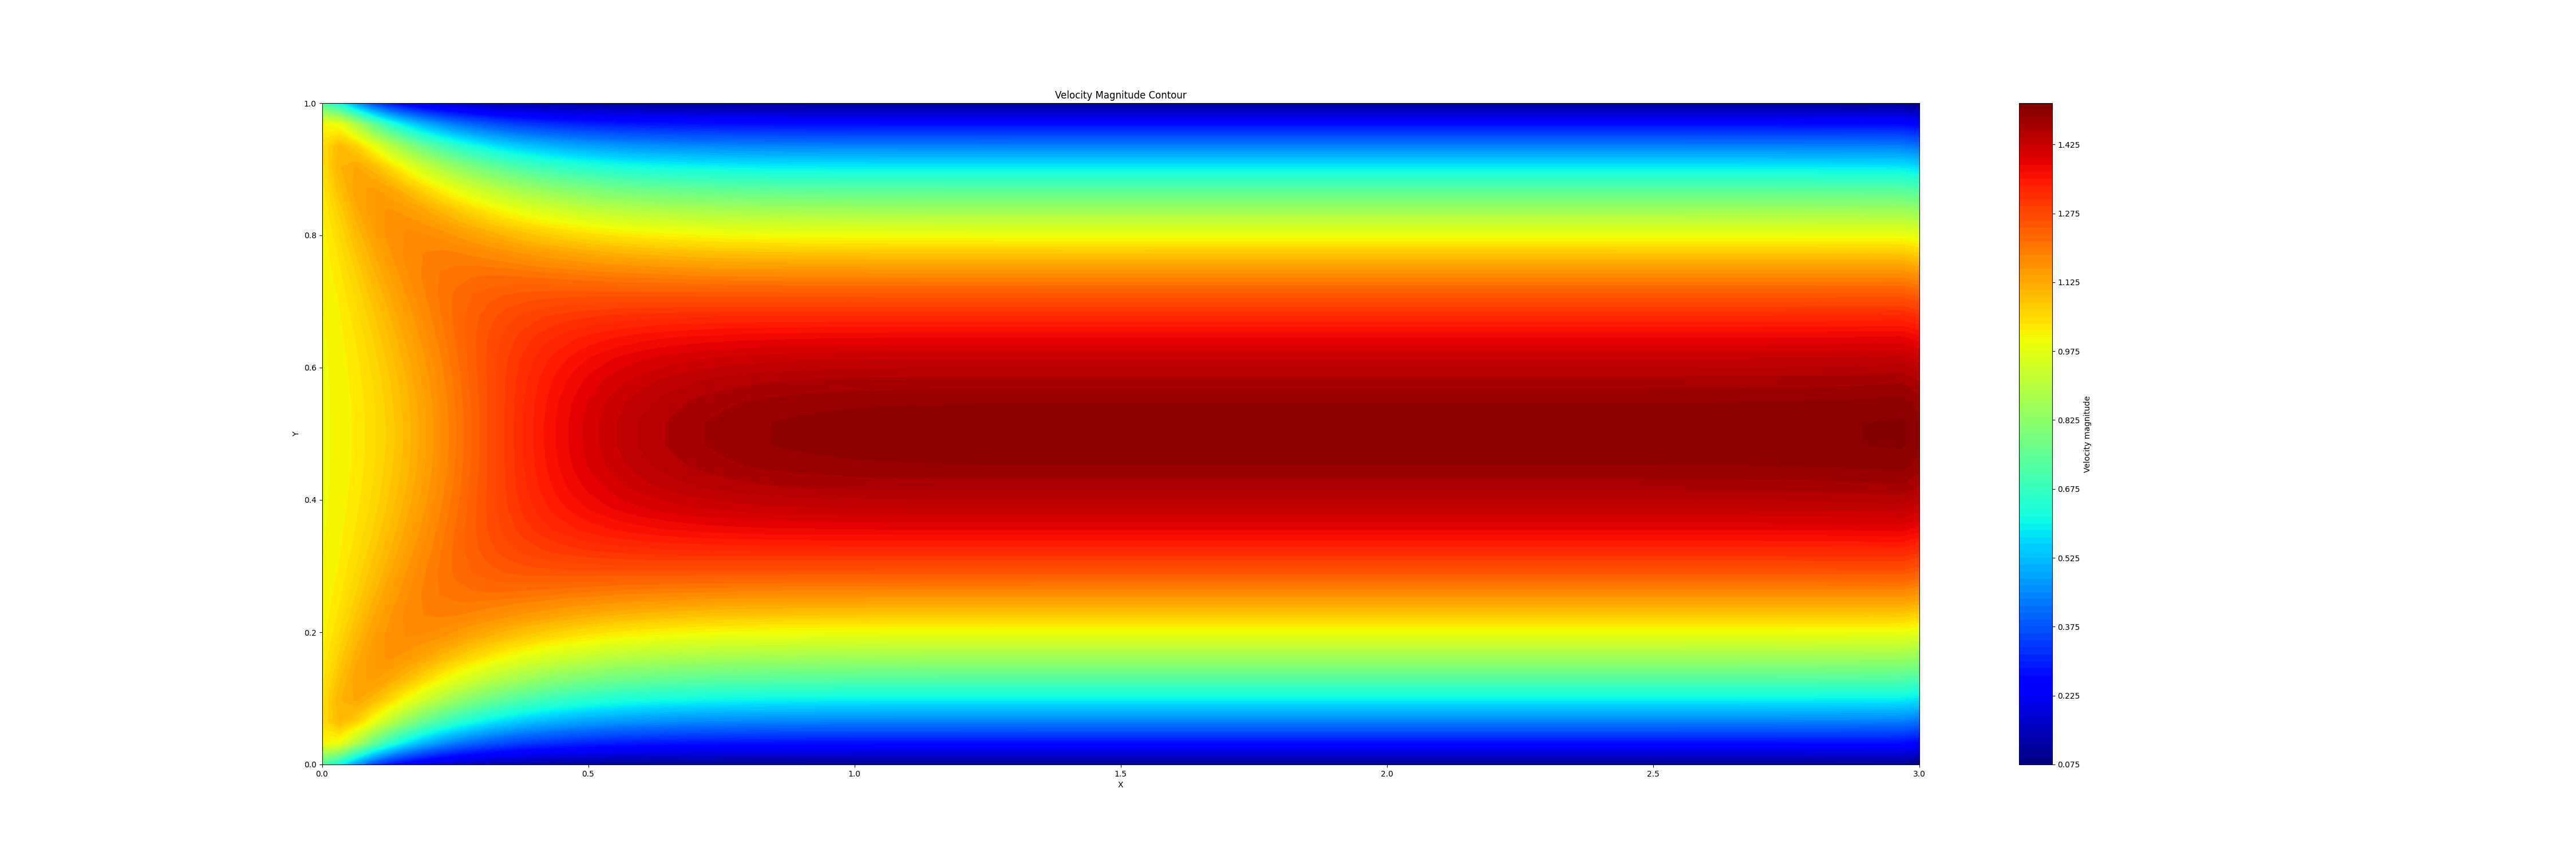
\includegraphics[width=1.2\linewidth]{figure/Channel_flow/cyl_uv_contour_N=32, Re=10, t=10.jpg}
    \caption{Velocity contour at t=50s}
\end{figure}

This diagram showed the velocity contour at t=50s, we could observe it do develop boundary layer and fully developed after certain length, and velocity have maximum value at the center of the channel.


\begin{figure}[H]
    \centering
    
\includegraphics[width=1.2\linewidth]{figure/Channel_flow/ductflow_p_contour_N=32.jpg}
    \caption{Pressure contour}
\end{figure}



\subsubsection{Comparison with theoretical solution}

To check our result's precision, we checked our result with the theoretical solution, where the channel flow's theoretically solution is showing below:
$$
u_{\text{exact}} = U \left(1 - \left(\frac{y - 0.5}{0.5}\right)^2\right)
$$

We compare this result with our numerical result, could find our numerical result is close to the exact solution:

\begin{figure}[H]
    \centering
    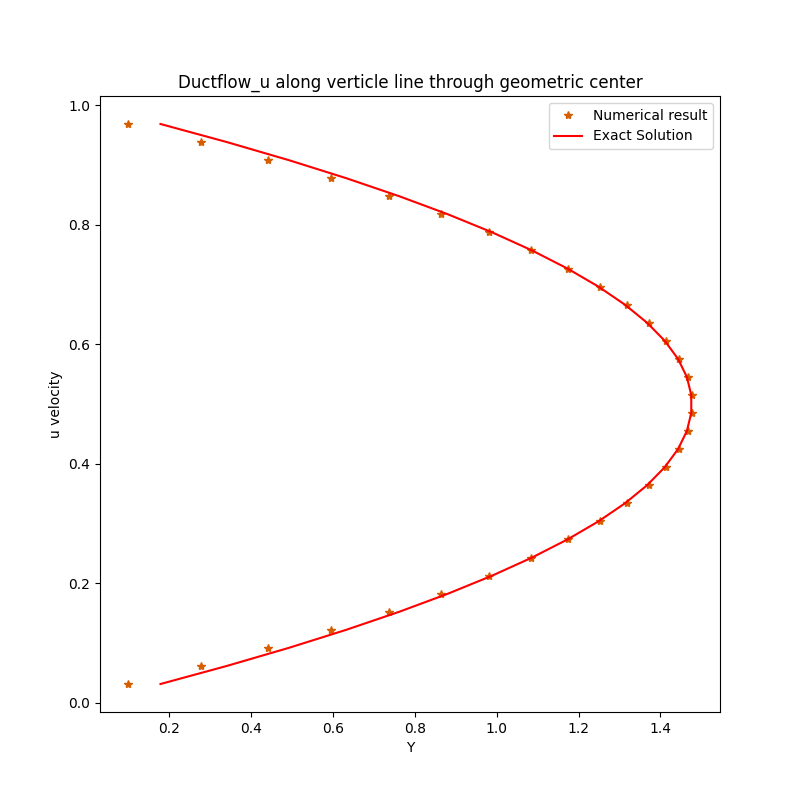
\includegraphics[width=0.6\linewidth]{figure/Channel_flow/Ductflow_u along verticle line through geometric center.jpg}
    \caption{u comparison}
\end{figure}




























\newpage
\section{Re=150--Circular cylinder in a cross-flow}
\subsection{Settings}

\begin{figure}[H]
    \centering
    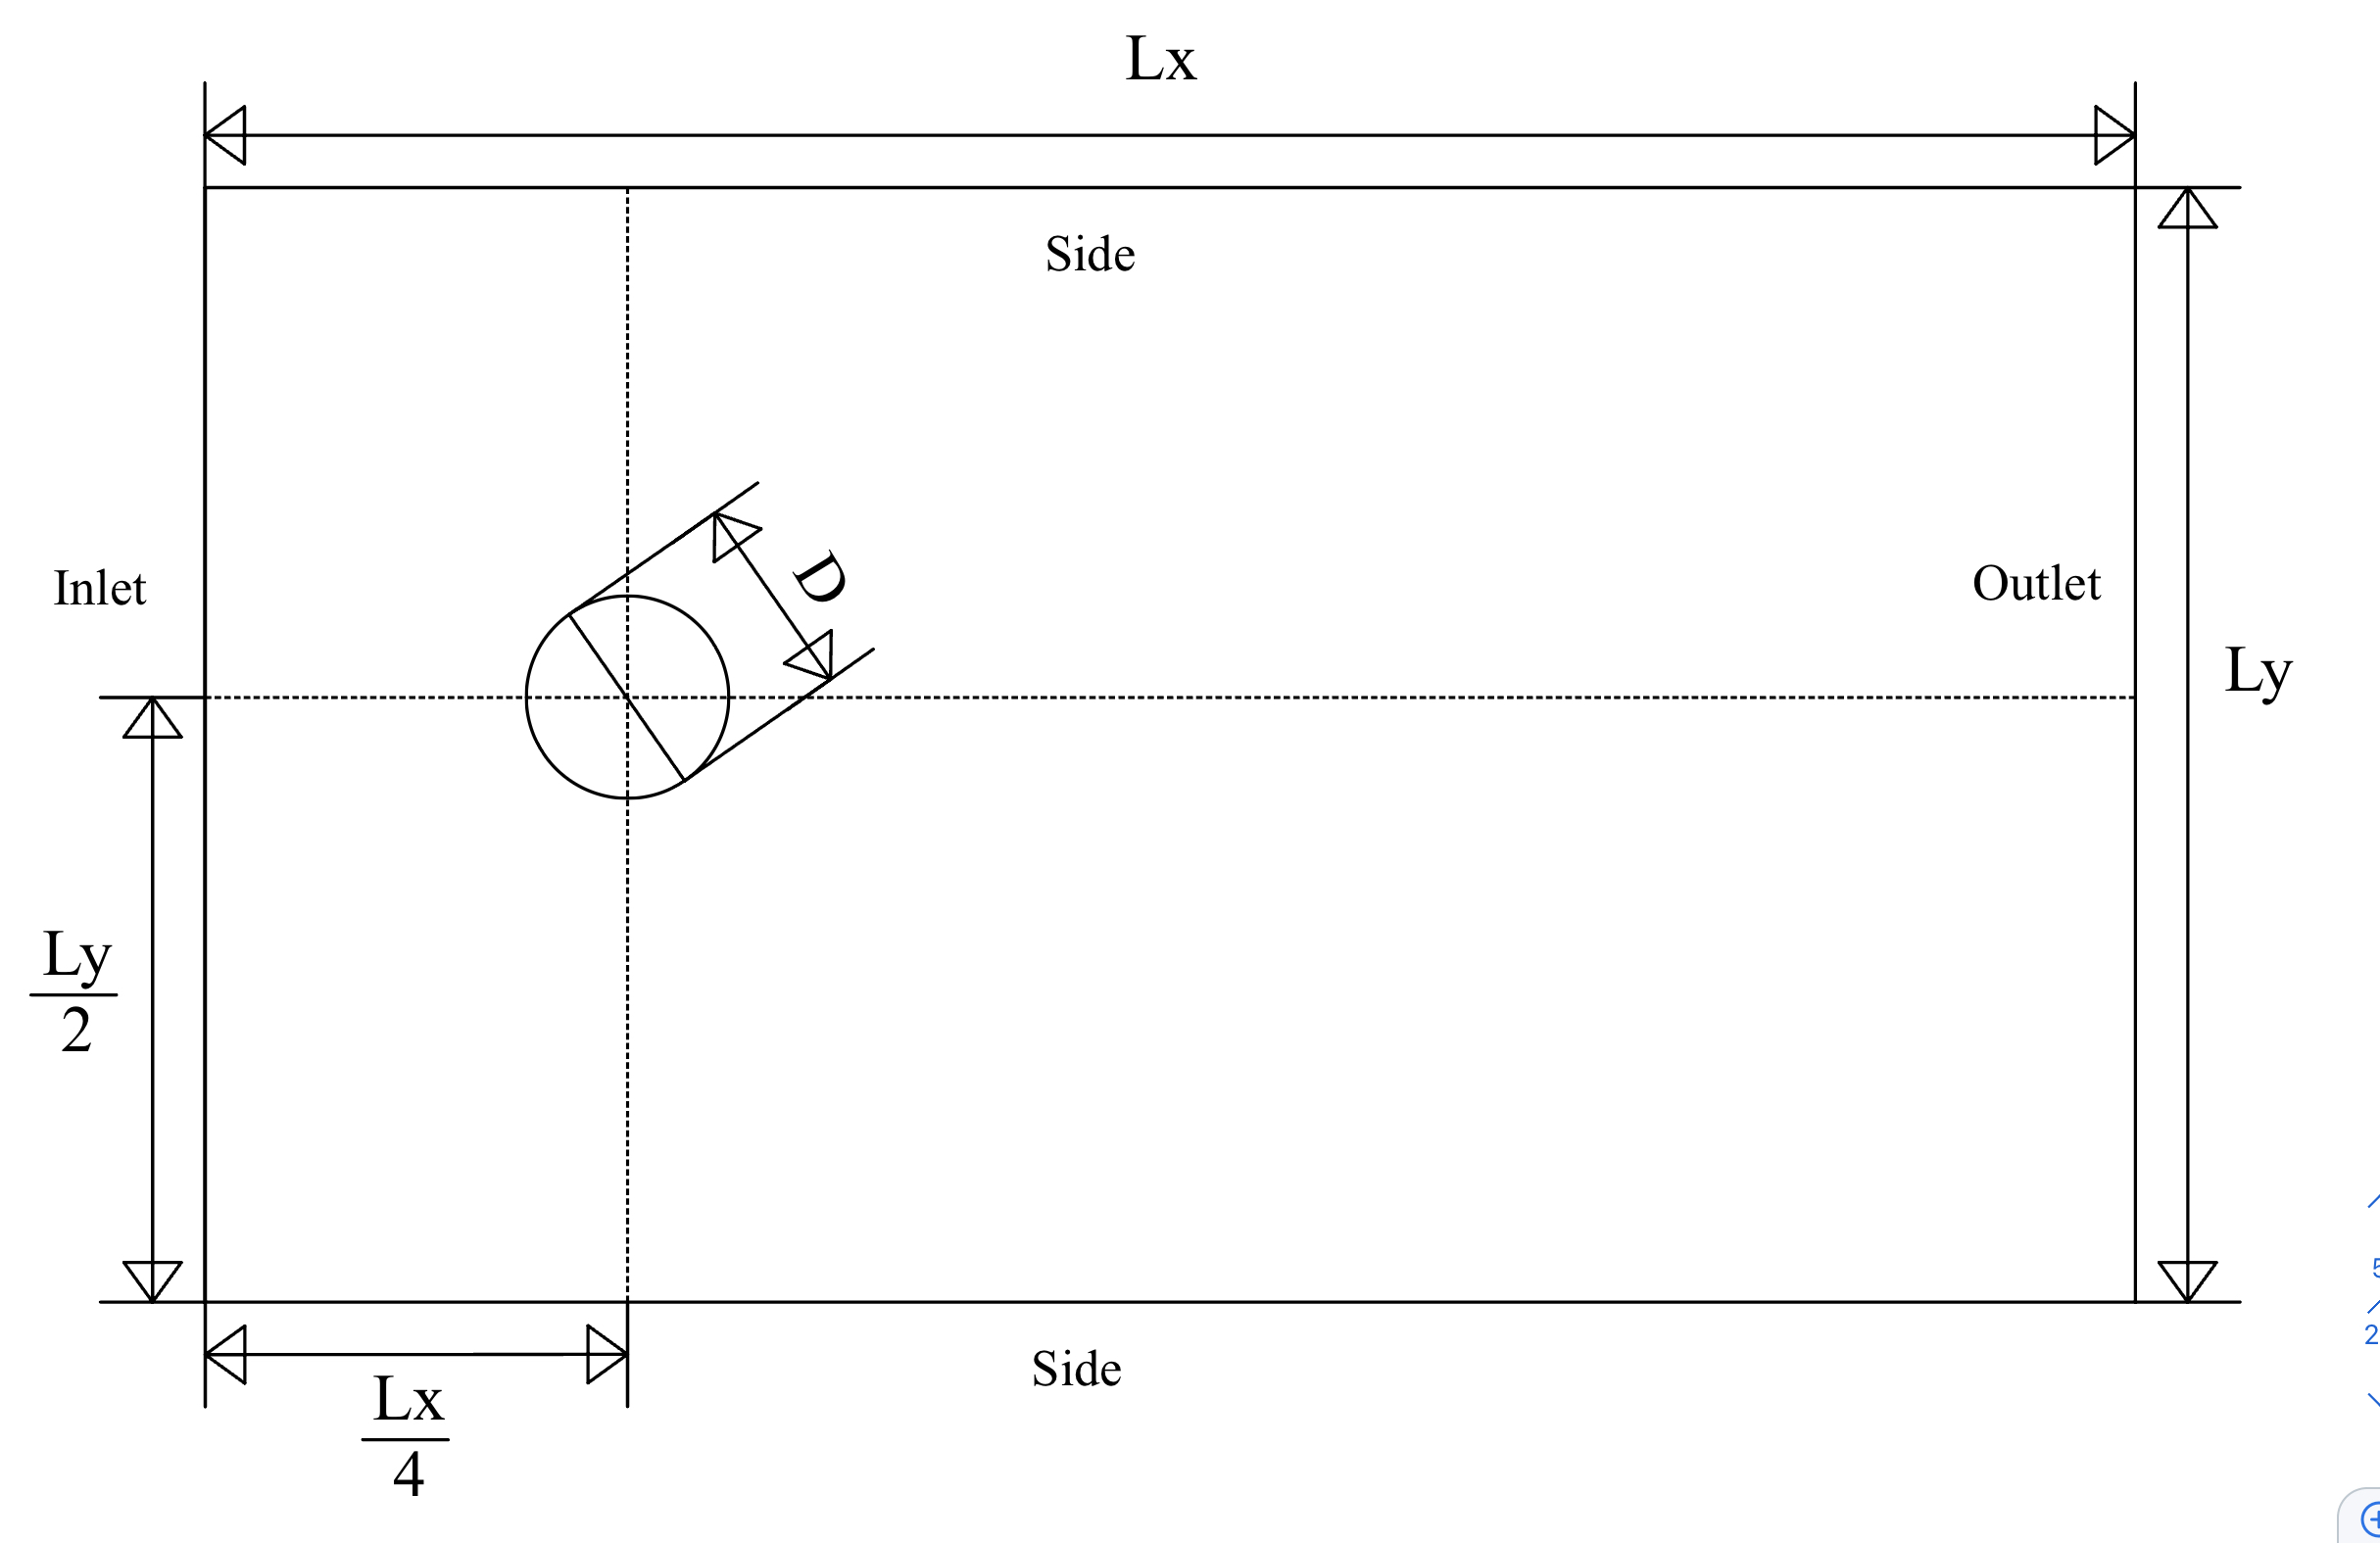
\includegraphics[width=0.6\linewidth]{figure/Solver and Stting/Cylinder_Setting.jpg}
    \caption{Domain and boundary setting for circular cylinder}
\end{figure}

The Domain setting as shown above. The key parameters as follows:
\begin{itemize}
    \item \textbf{Ly=4, Lx=8}: Width and Length of the domain
    \item \textbf{Circle Center}: the location of circular cylinder center=$(\frac{Lx}{4}, \frac{Ly}{2})$
    \item  \textbf{D=0.5}: The diameter of the circle

    \item \textbf{Inlet}: $u=1, v=0, \frac{\partial p}{\partial x}=0$
    \item \textbf{Side}: $\frac{\partial u}{\partial y}=0, \frac{\partial v}{\partial y}=0, 
    \frac{\partial p}{\partial y}=0$
    \item \textbf{Outlet}: $\frac{\partial u}{\partial x}=0, \frac{\partial v}{\partial x}=0, 
    \frac{\partial p}{\partial x}=0$
\end{itemize}







\subsection{Result among time}

\subsubsection{t=10 and t=50}
By setting the parameters as the chapter shown before, we now exhibit the result of t=10 and t=100 as follows:

\begin{figure}[H]
    \centering
    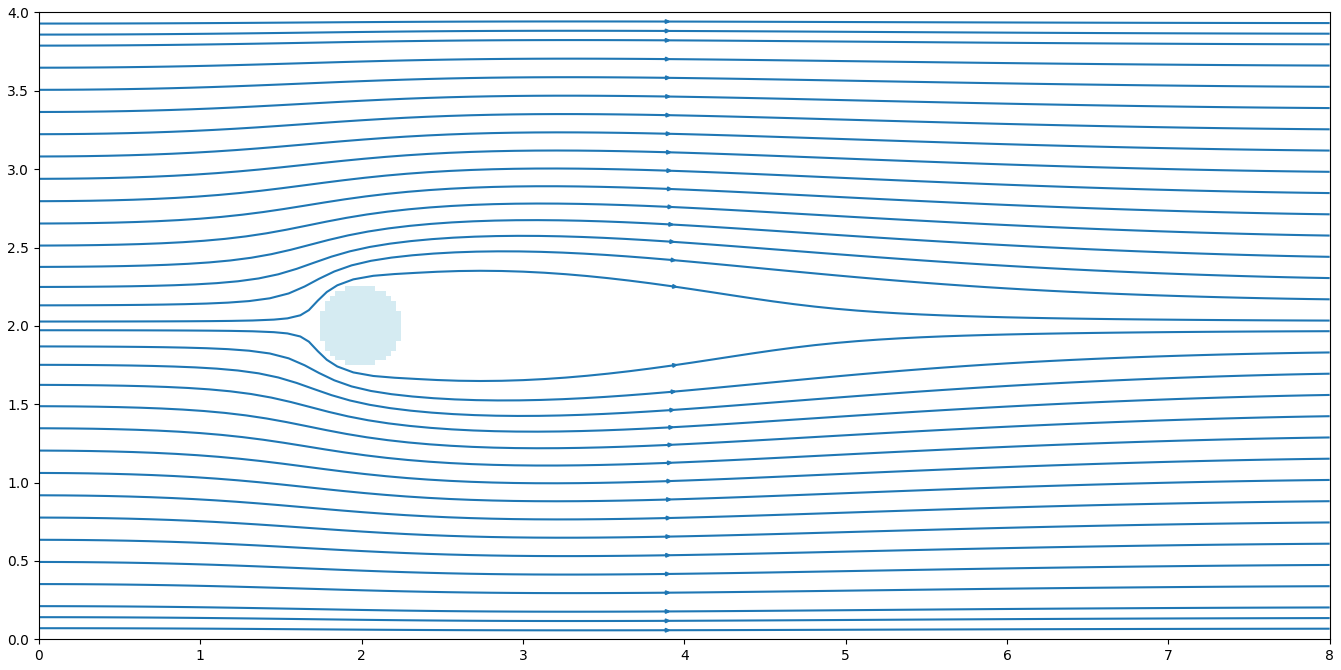
\includegraphics[width=0.45\linewidth]{figure/N32_Re150_8x4_t10/stline_N32_Re150_8x4_t10.jpg}
    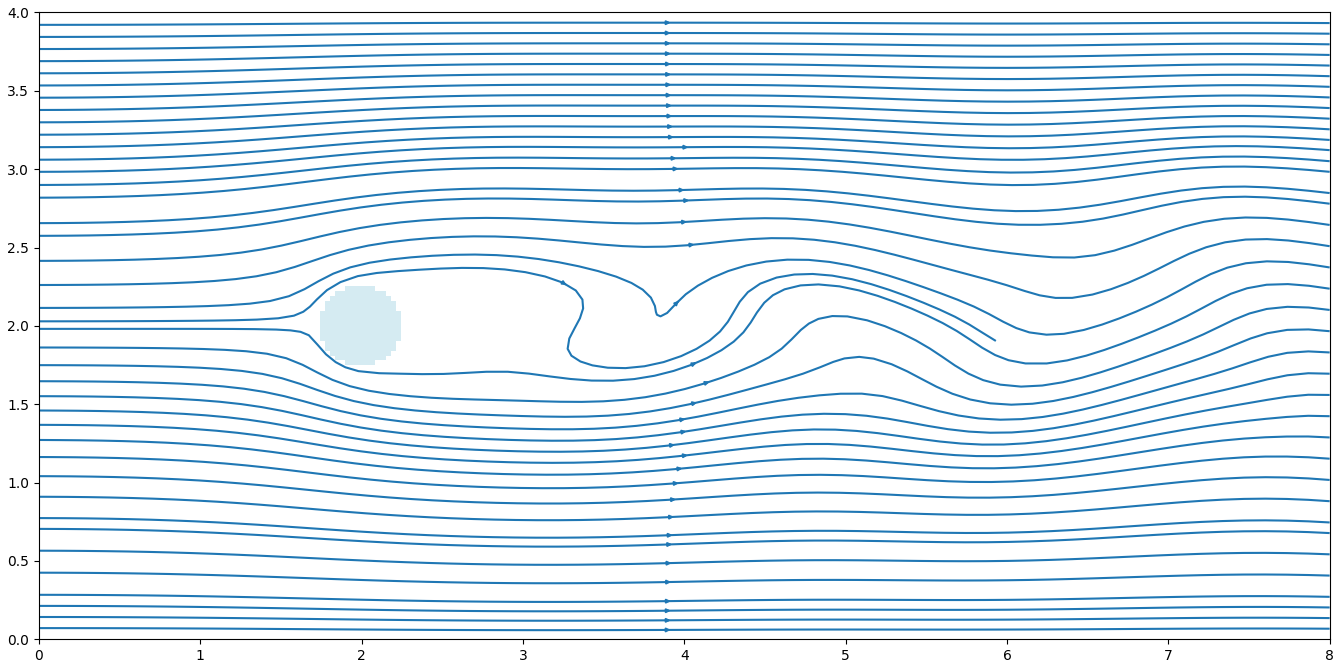
\includegraphics[width=0.45\linewidth]{figure/N32_Re150_8x4_t50/stline_N32_Re150_8x4_t50.jpg}
    \caption{Streamline at t=10 (left), Streamline at t=10 t=50s (right)}
\end{figure}


Based on the figures shows for t=10 and t=50, we could find at t=10, the flow is kind of steady, where is shows the flow have not been disturbed, and flow pattern is symmetric along y-direction.

\begin{figure}[H]
    \centering
    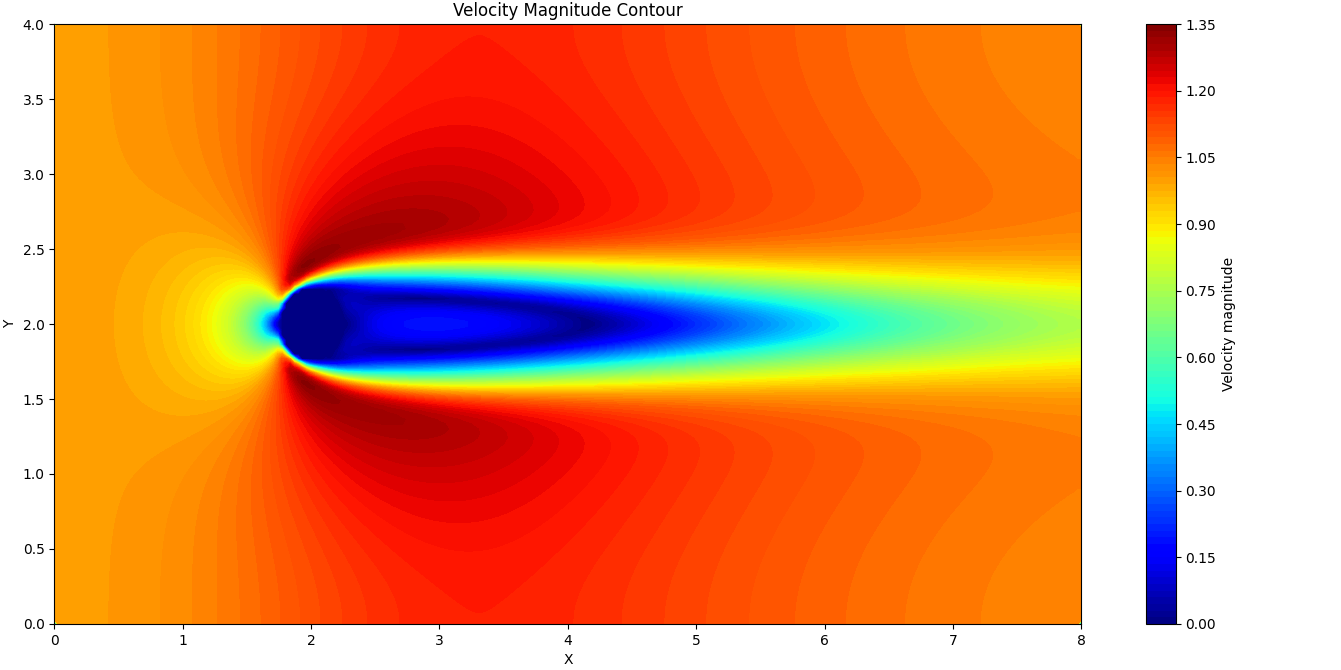
\includegraphics[width=0.45\linewidth]{figure/N32_Re150_8x4_t10/v_N32_Re150_8x4_t10.jpg}
    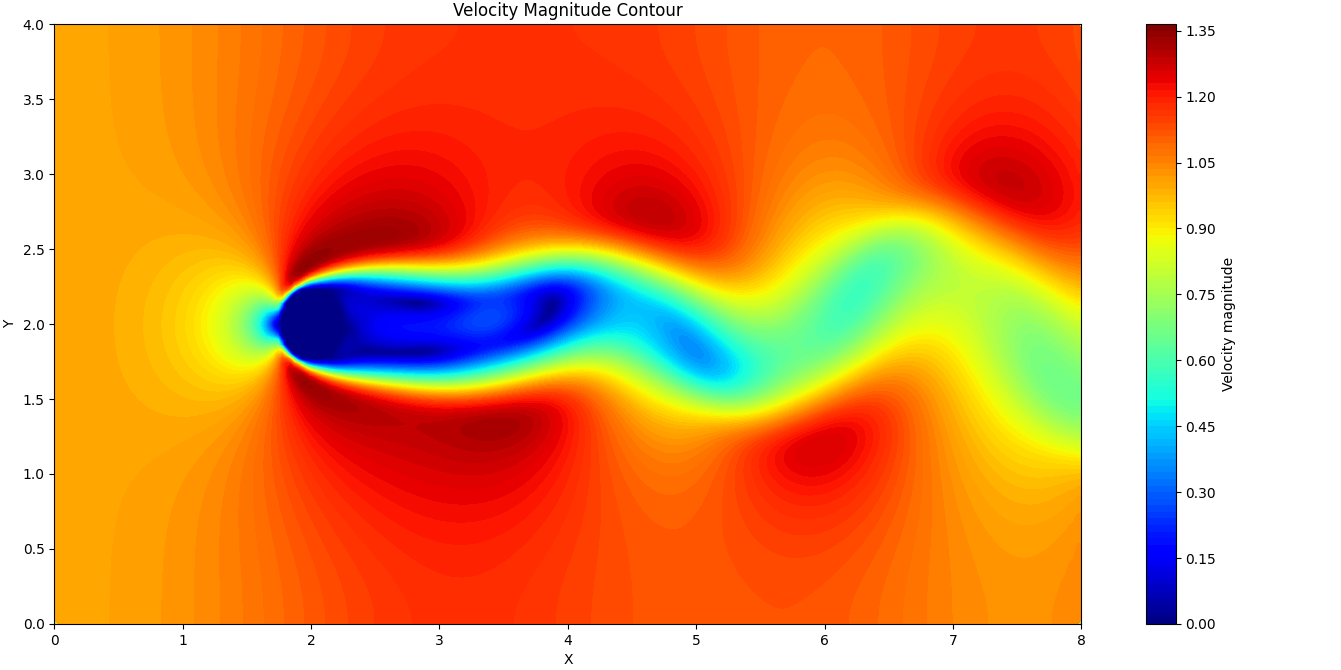
\includegraphics[width=0.45\linewidth]{figure/N32_Re150_8x4_t50/v_N32_Re150_8x4_t50.jpg}
    \caption{Velocity at t=10 (left), Pressure at t=10 t=50s (right)}
\end{figure}




\begin{figure}[H]
    \centering
    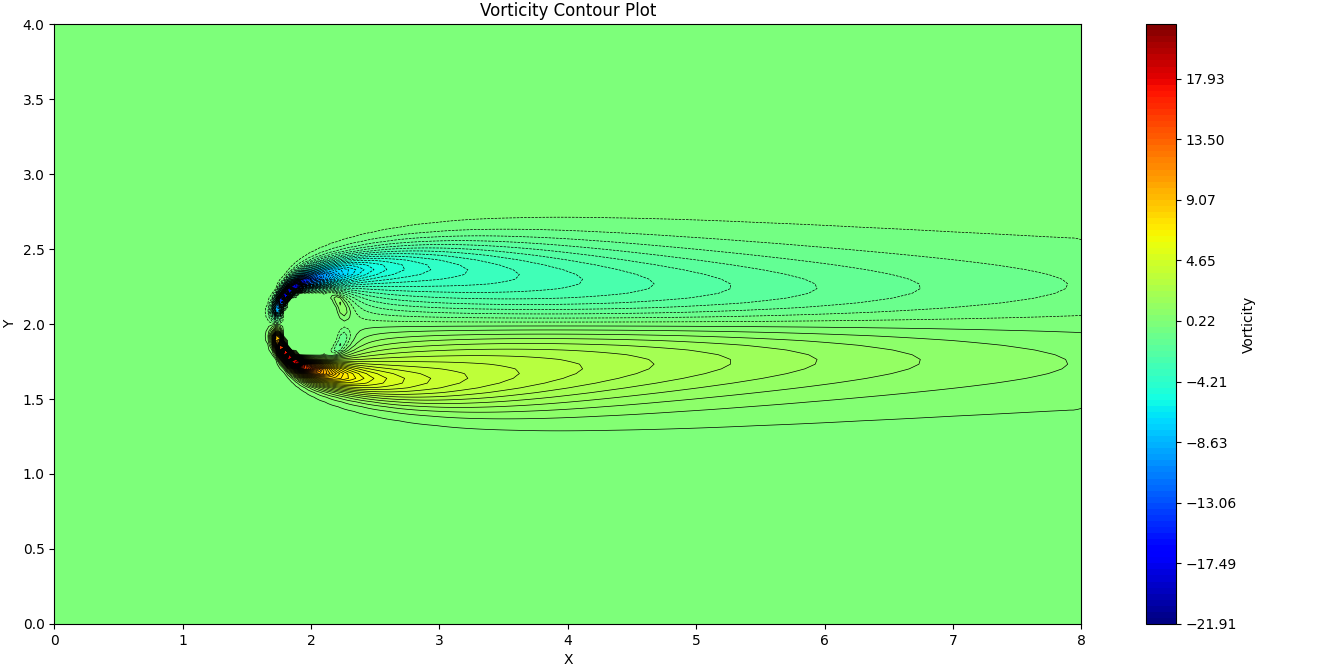
\includegraphics[width=0.45\linewidth]{figure/N32_Re150_8x4_t10/vor_N32_Re150_8x4_t10.jpg}
    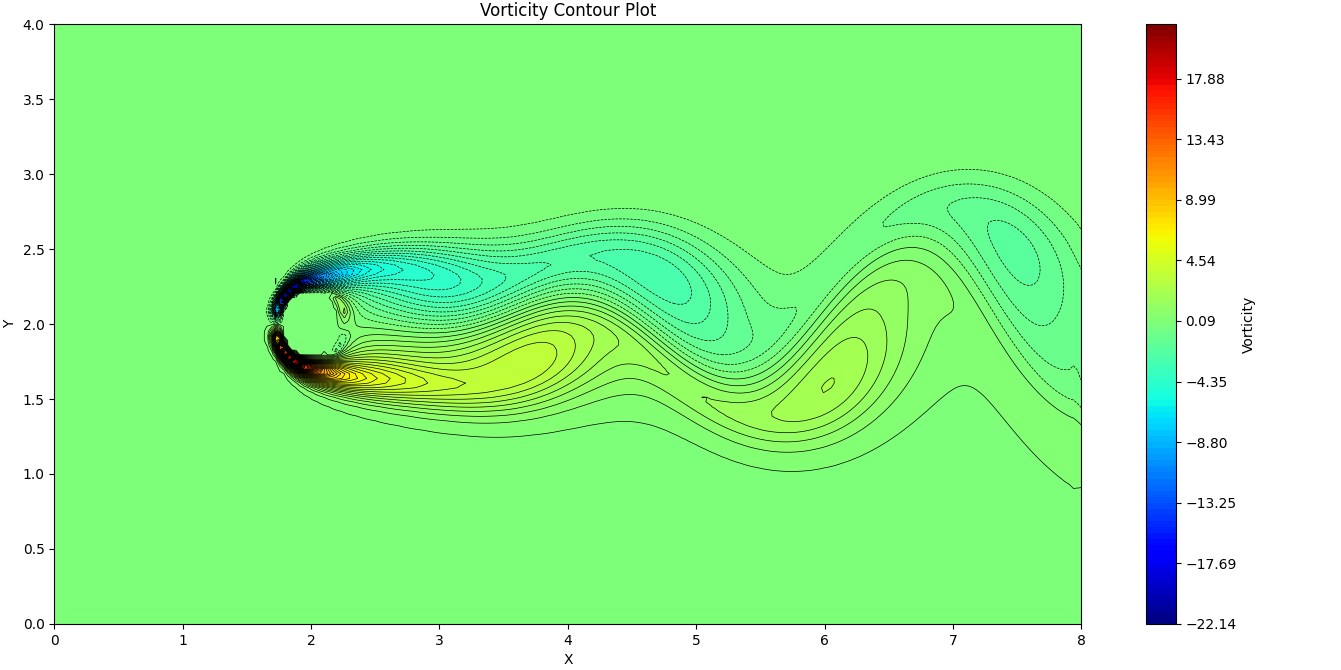
\includegraphics[width=0.45\linewidth]{figure/N32_Re150_8x4_t50/vor_N32_Re150_8x4_t50.jpg}
    \caption{Vorticity at t=10 (left), Vorticity at t=10 t=50s (right)}
\end{figure}

The same result shown in vorticity contour and pressure contour, where we could find the flow is not symmetric and start to show voticies.

\begin{figure}[H]
    \centering
    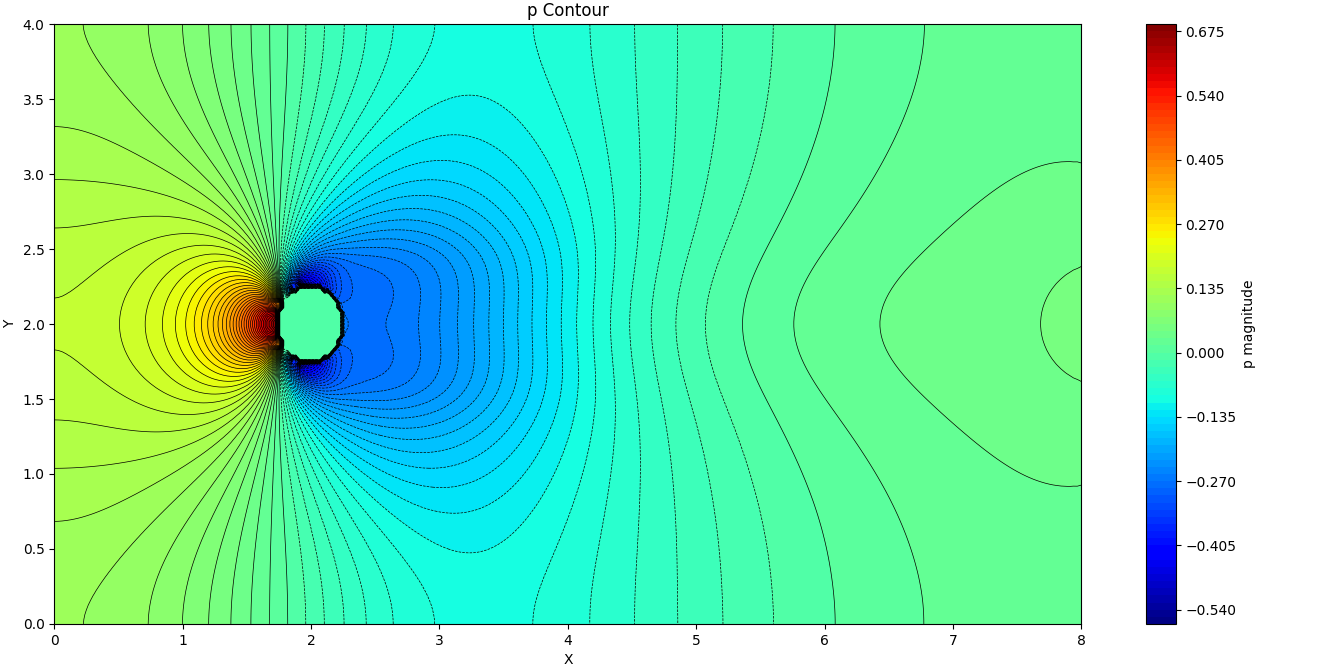
\includegraphics[width=0.45\linewidth]{figure/N32_Re150_8x4_t10/p_N32_Re150_8x4_t10.jpg}
    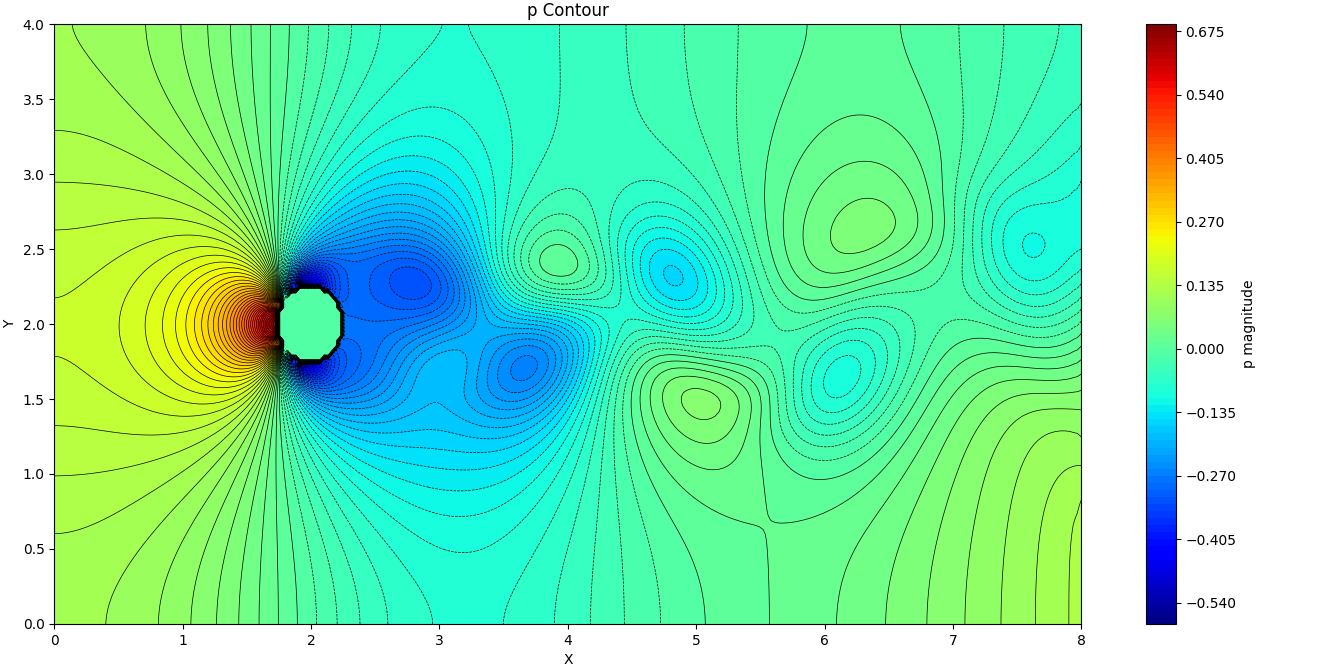
\includegraphics[width=0.45\linewidth]{figure/N32_Re150_8x4_t50/p_N32_Re150_8x4_t50.jpg}
    \caption{Pressure at t=10 (left), Pressure at t=50s (right)}
\end{figure}






\subsubsection{t=50 and t=100}
By setting the parameters as the chapter shown before, we now exhibit the result of t=50 and t=100 as follows:

\begin{figure}[H]
    \centering
    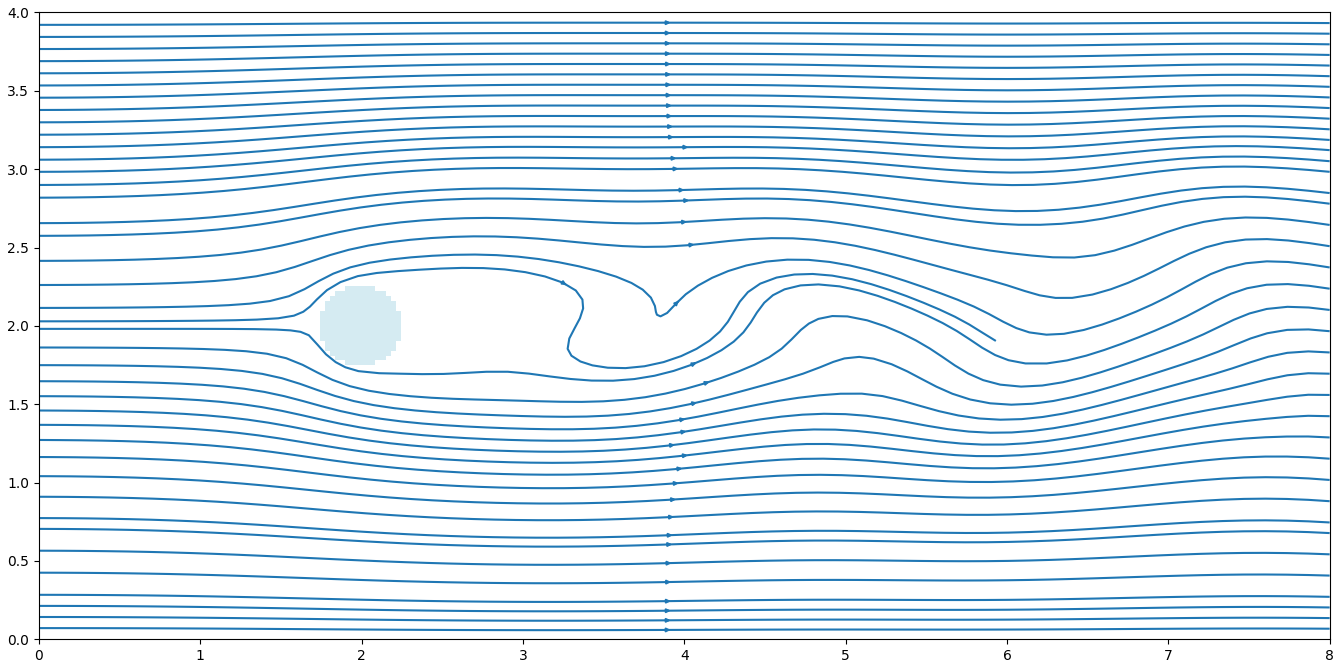
\includegraphics[width=0.45\linewidth]{figure/N32_Re150_8x4_t50/stline_N32_Re150_8x4_t50.jpg}
    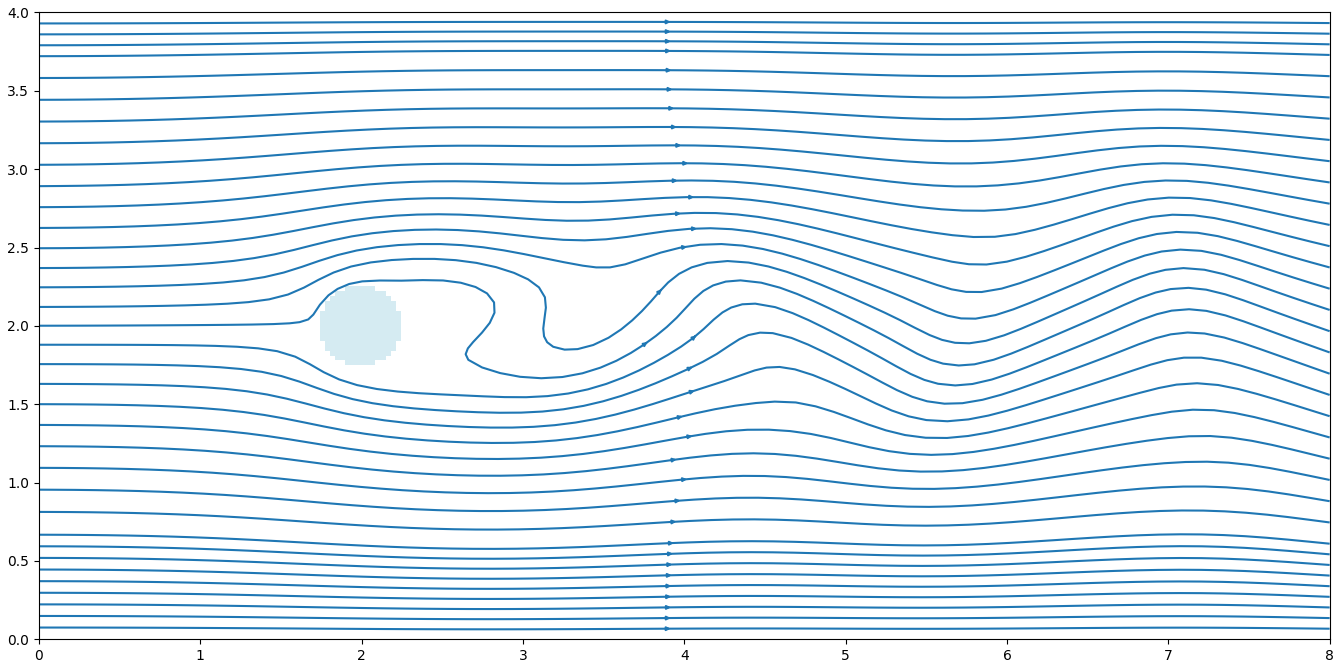
\includegraphics[width=0.45\linewidth]{figure/N32_Re150_8x4_t100/stline_N32_Re150_8x4_t100.jpg}
    \caption{Streamline at t=50 (left), Streamline at t=10 t=100s (right)}
\end{figure}

Form t=50 to t=100, we could also find that the vortex is shedding from cylinder and let the flow more unsteady.

\begin{figure}[H]
    \centering
    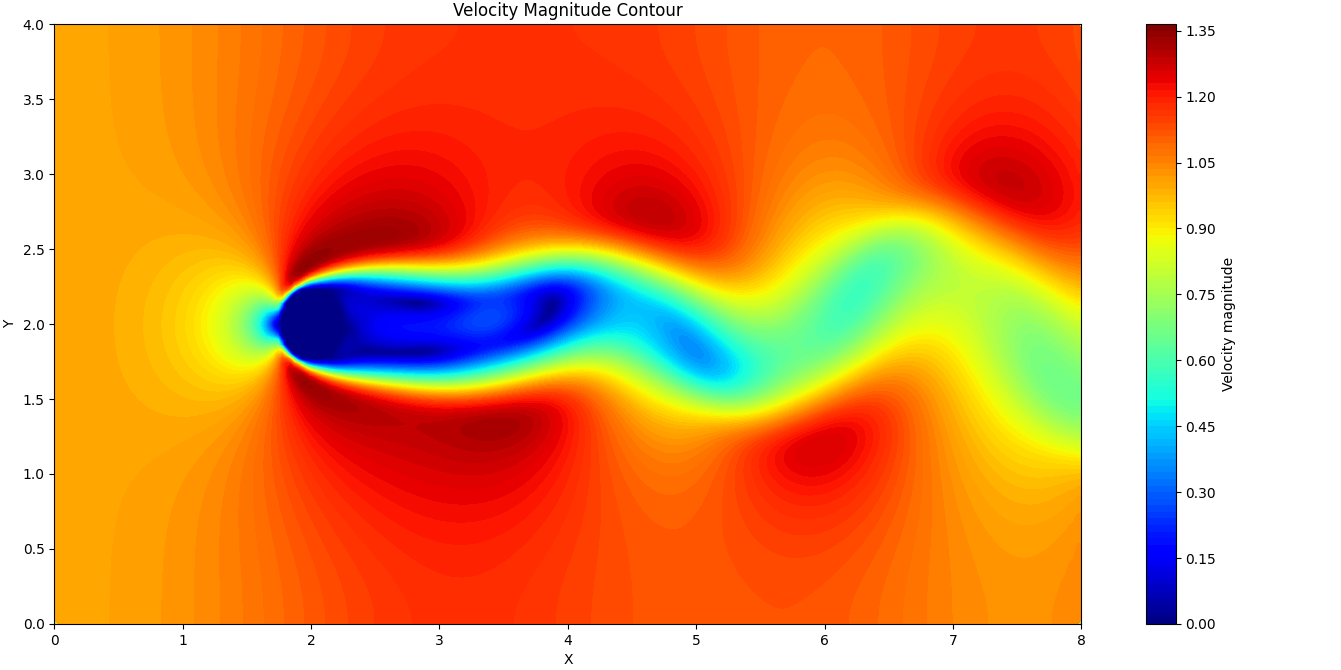
\includegraphics[width=0.45\linewidth]{figure/N32_Re150_8x4_t50/v_N32_Re150_8x4_t50.jpg}
    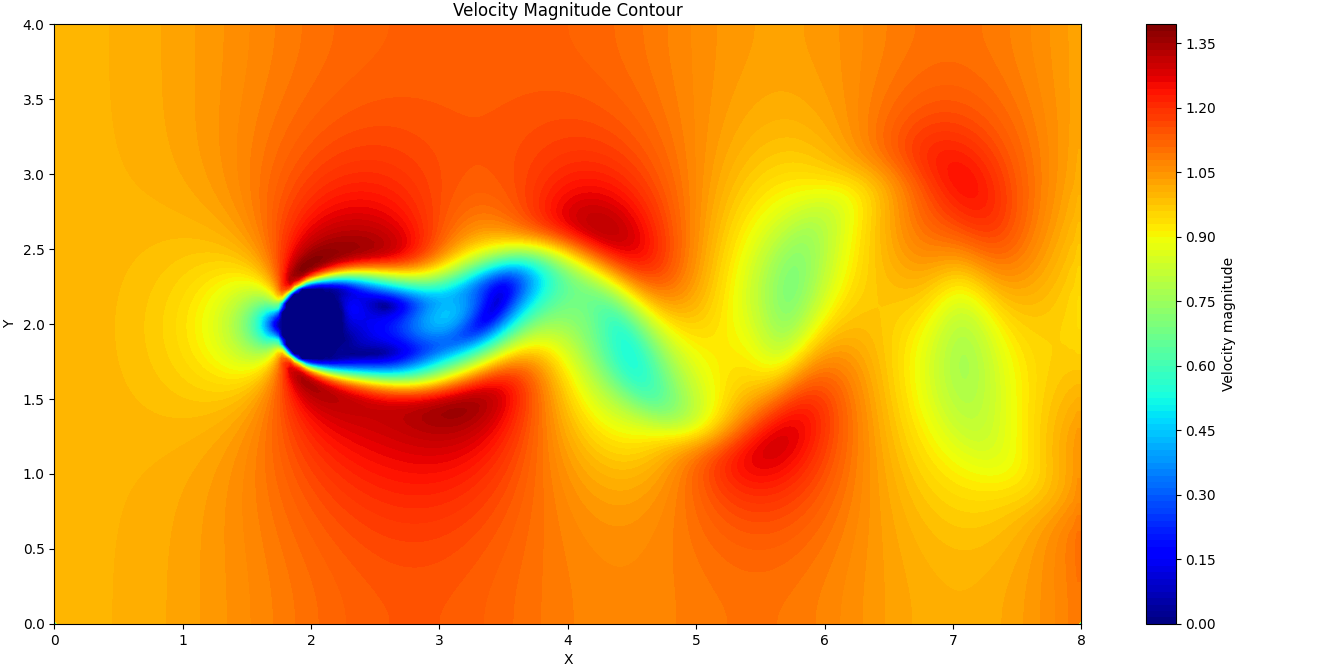
\includegraphics[width=0.45\linewidth]{figure/N32_Re150_8x4_t100/v_N32_Re150_8x4_t100.jpg}
    \caption{Velocity at t=50 (left), Pressure at t=10 t=100s (right)}
\end{figure}



\begin{figure}[H]
    \centering
    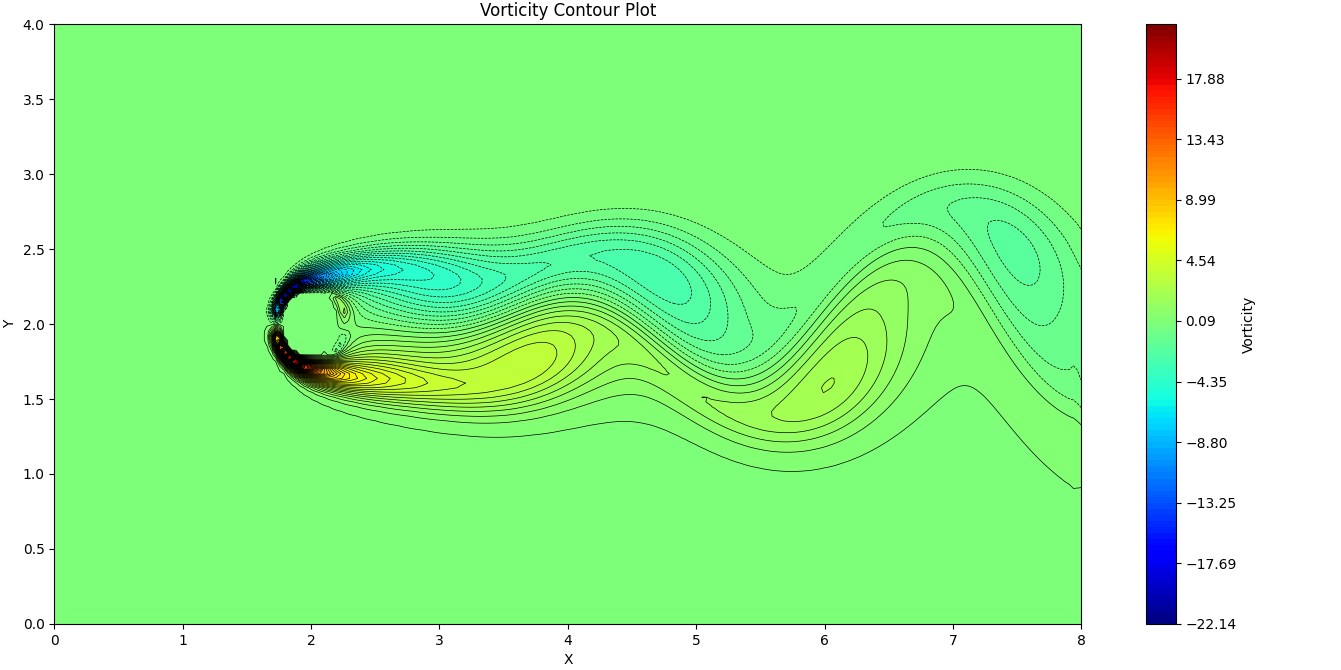
\includegraphics[width=0.45\linewidth]{figure/N32_Re150_8x4_t50/vor_N32_Re150_8x4_t50.jpg}
    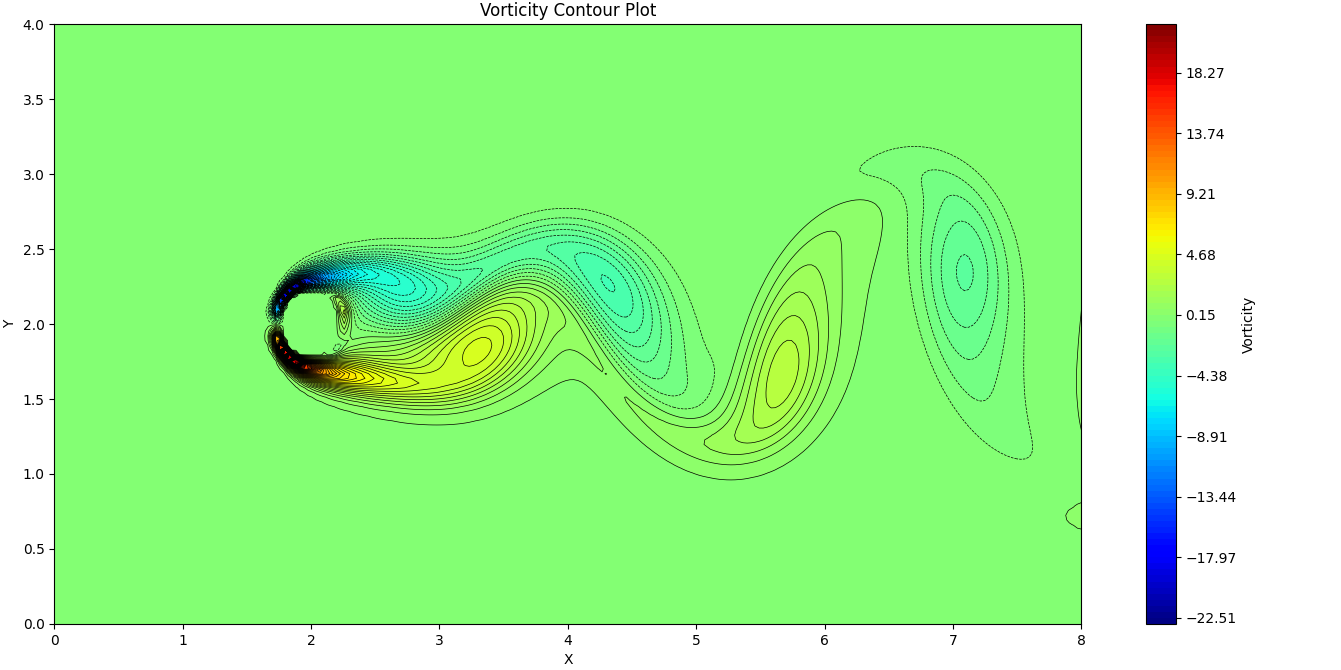
\includegraphics[width=0.45\linewidth]{figure/N32_Re150_8x4_t100/vor_N32_Re150_8x4_t100.jpg}
    \caption{Vorticity at t=50 (left), Vorticity at t=100s (right)}
\end{figure}

From these result, we could see small vortices lying up along y-center side.

\begin{figure}[H]
    \centering
    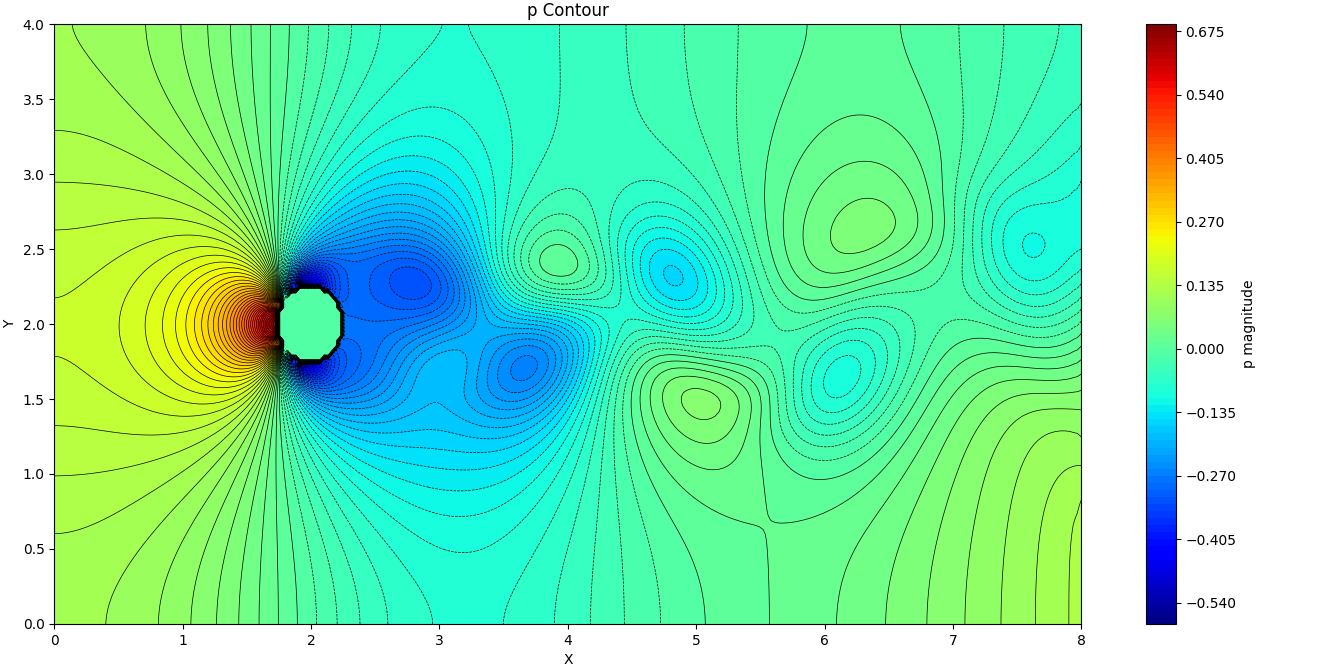
\includegraphics[width=0.45\linewidth]{figure/N32_Re150_8x4_t50/p_N32_Re150_8x4_t50.jpg}
    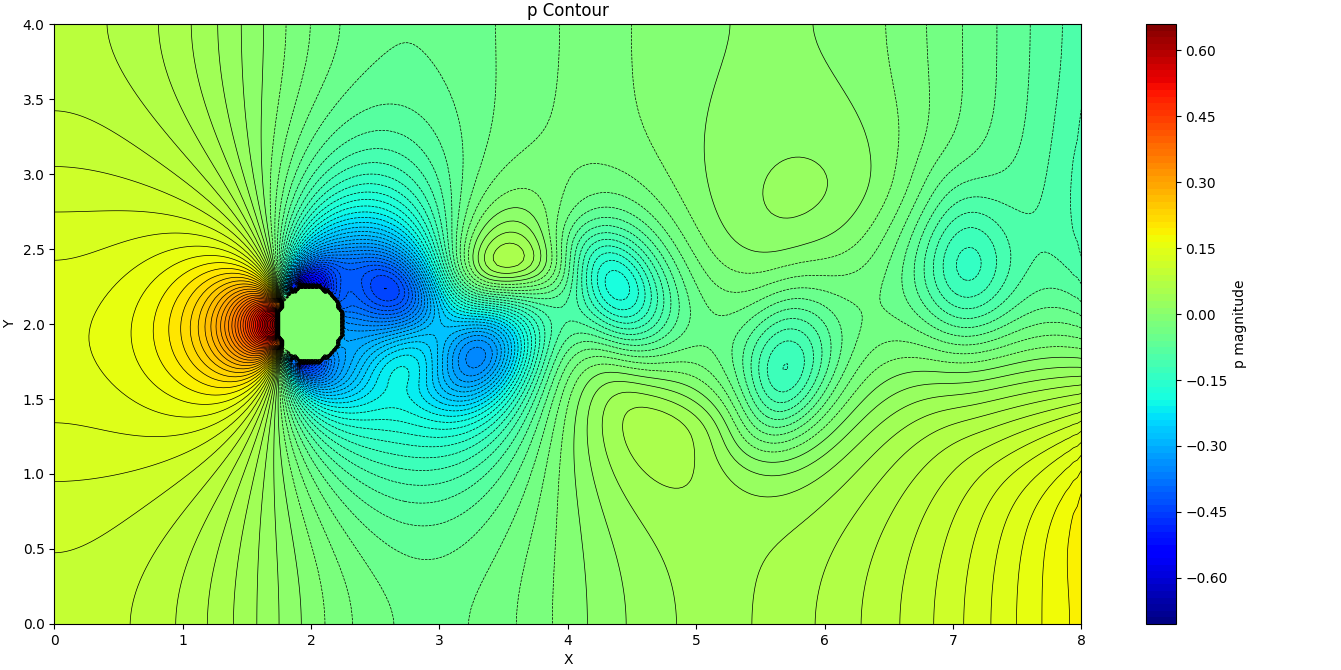
\includegraphics[width=0.45\linewidth]{figure/N32_Re150_8x4_t100/p_N32_Re150_8x4_t100.jpg}
    \caption{Pressure at t=50 (left), Pressure at t=100s (right)}
\end{figure}

From the figure of pressure contour, we could noticed that the pressure shows its maximum at the front point of the circle, and the minimum (negative) at the back of the circle. While the vortex shedding showing up, we could find a similar pattern of the vortex, velocity and pressure contour arrangement.









\subsubsection{Result Comparison of time (t=10, 50, and 100)}

To get more comprehensive understanding of the vortex shedding among time, we let the result of t=10, t=50, and t=100 together as follows:

\begin{figure}[H]
    \centering
    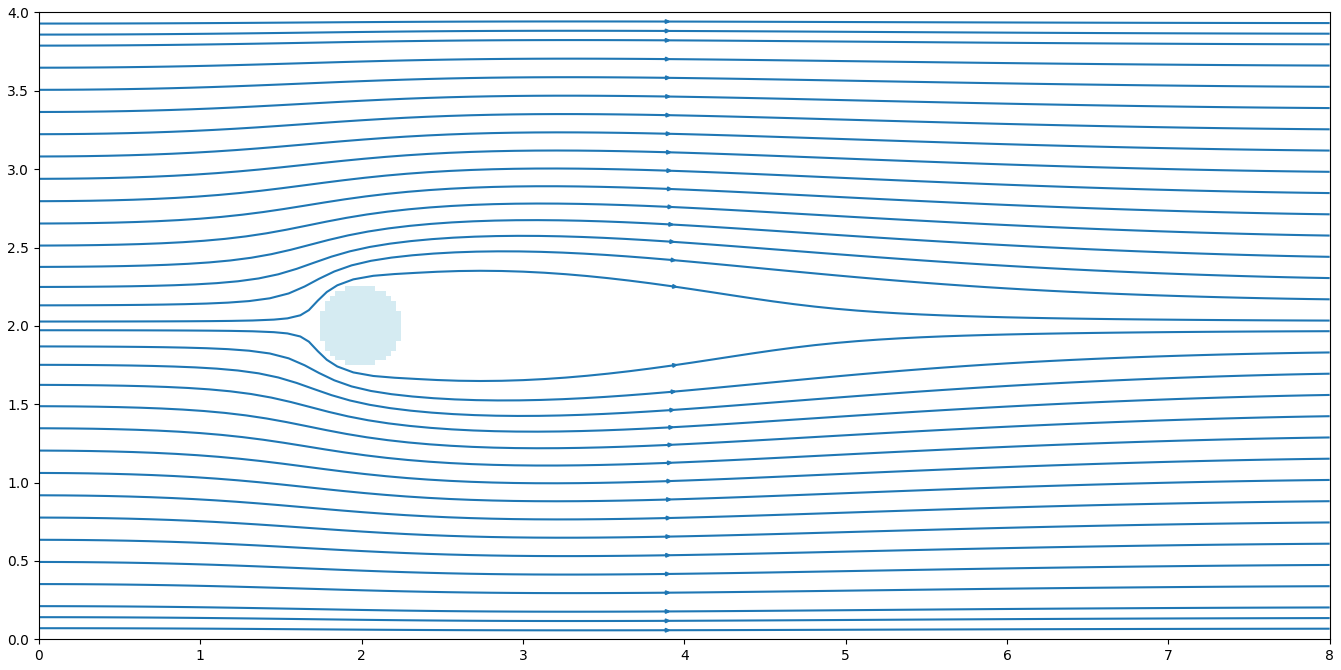
\includegraphics[width=0.3\linewidth]{figure/N32_Re150_8x4_t10/stline_N32_Re150_8x4_t10.jpg}
    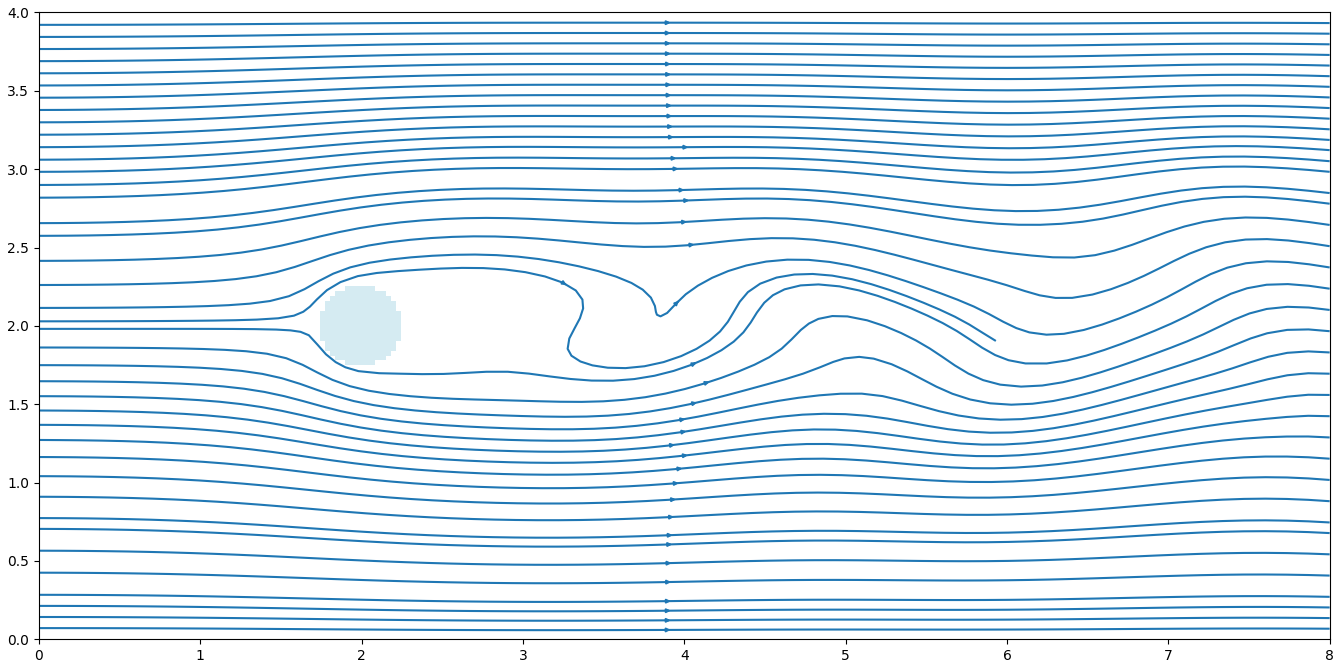
\includegraphics[width=0.3\linewidth]{figure/N32_Re150_8x4_t50/stline_N32_Re150_8x4_t50.jpg}
    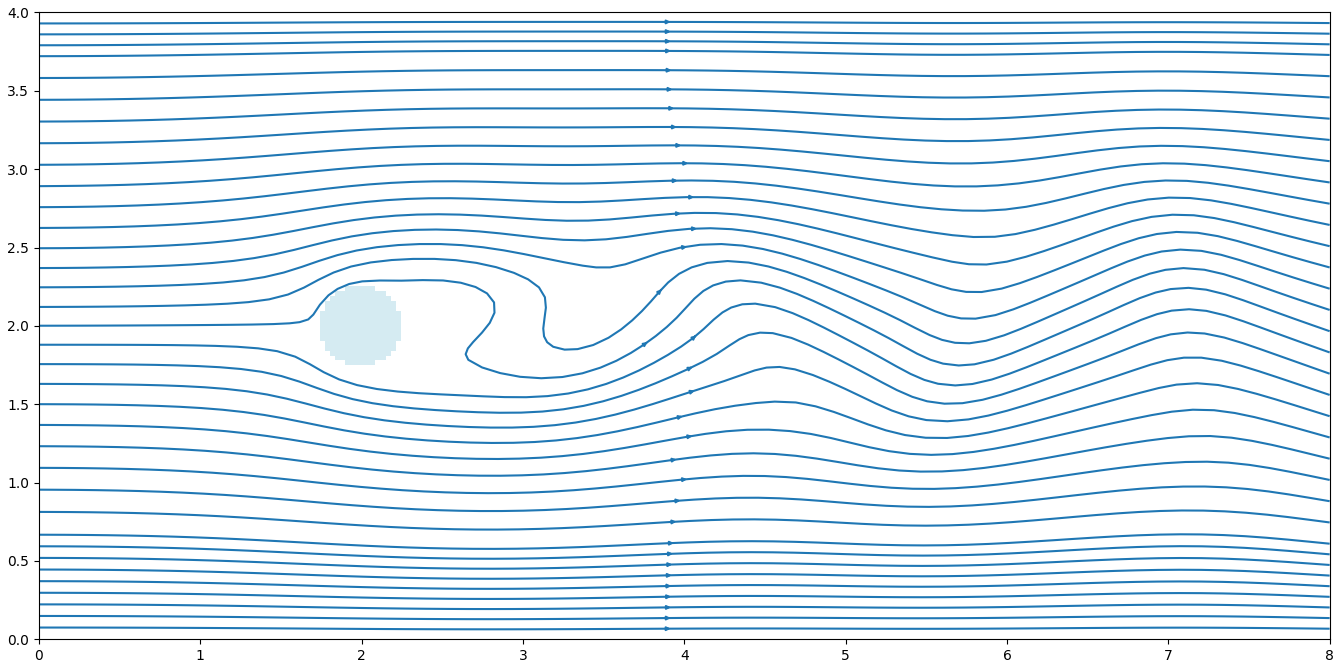
\includegraphics[width=0.3\linewidth]{figure/N32_Re150_8x4_t100/stline_N32_Re150_8x4_t100.jpg}
    \caption{Streamline at t=10 (left), t=50 (middle), t=100s (right)}
\end{figure}



\begin{figure}[H]
    \centering
    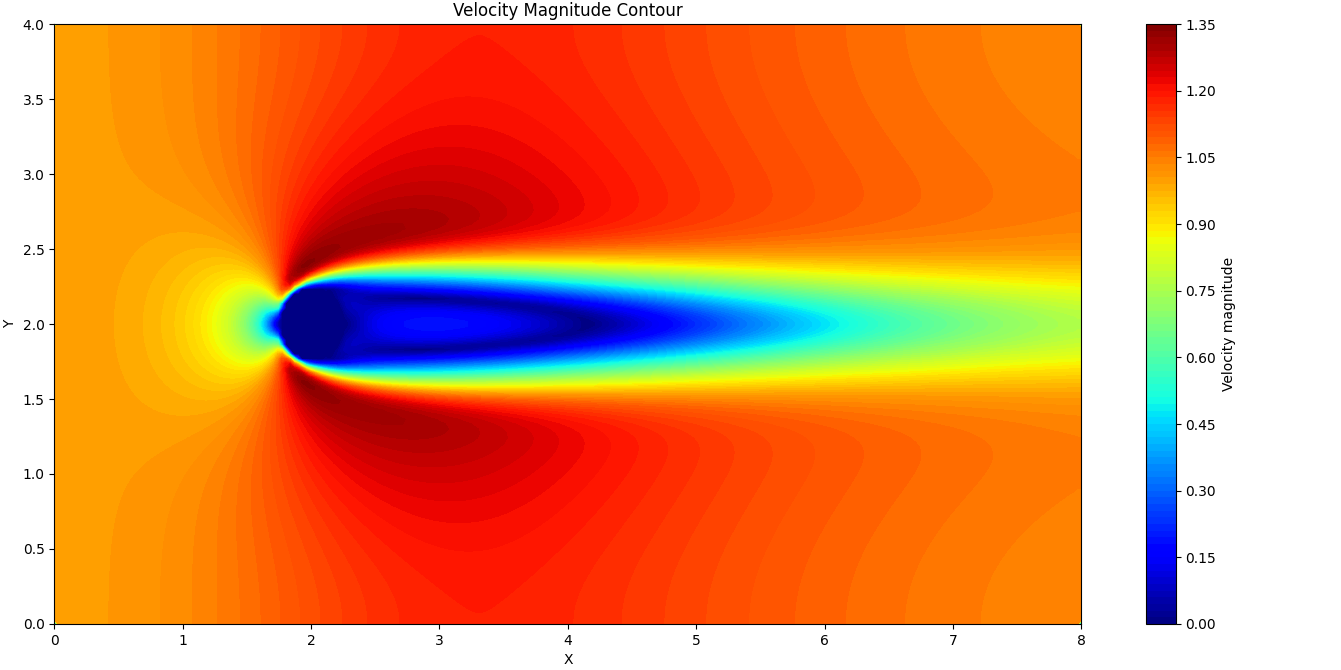
\includegraphics[width=0.3\linewidth]{figure/N32_Re150_8x4_t10/v_N32_Re150_8x4_t10.jpg}
    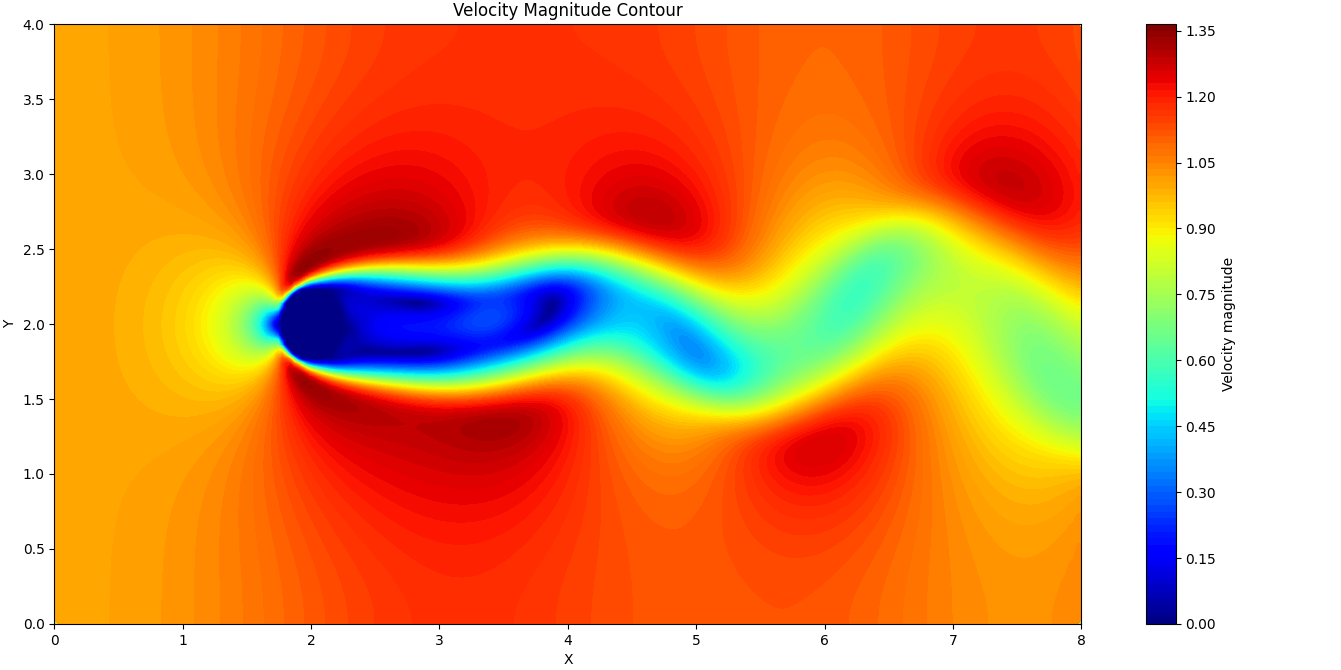
\includegraphics[width=0.3\linewidth]{figure/N32_Re150_8x4_t50/v_N32_Re150_8x4_t50.jpg}
    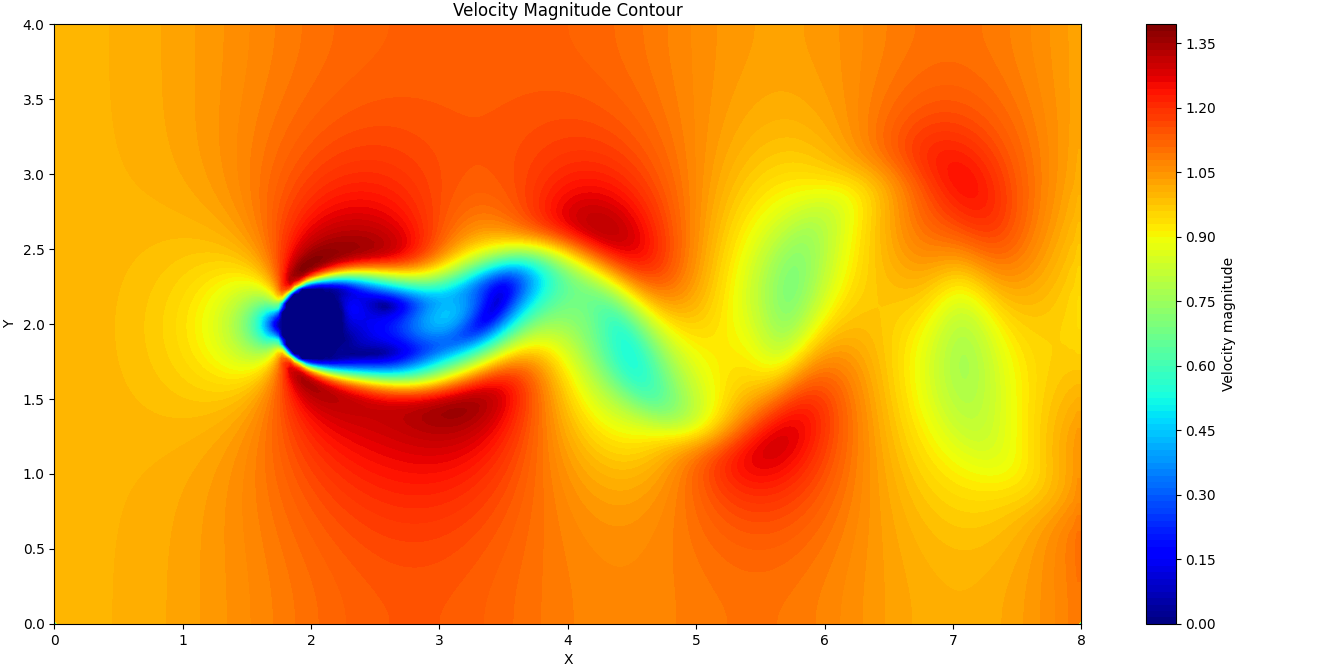
\includegraphics[width=0.3\linewidth]{figure/N32_Re150_8x4_t100/v_N32_Re150_8x4_t100.jpg}
    \caption{Velocity at t=10 (left), t=50 (middle), t=100s (right)}
\end{figure}

At t=100, we could observe the periodic behaviour typical of vortex shedding. 





\begin{figure}[H]
    \centering
    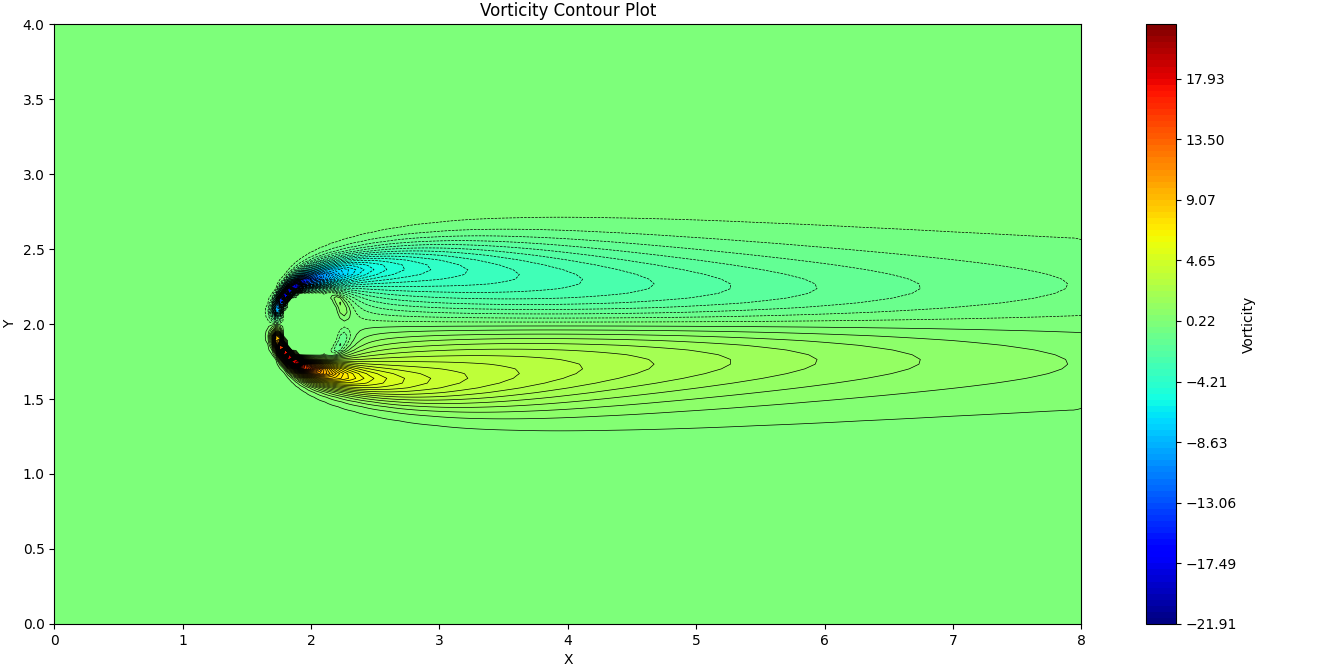
\includegraphics[width=0.3\linewidth]{figure/N32_Re150_8x4_t10/vor_N32_Re150_8x4_t10.jpg}
    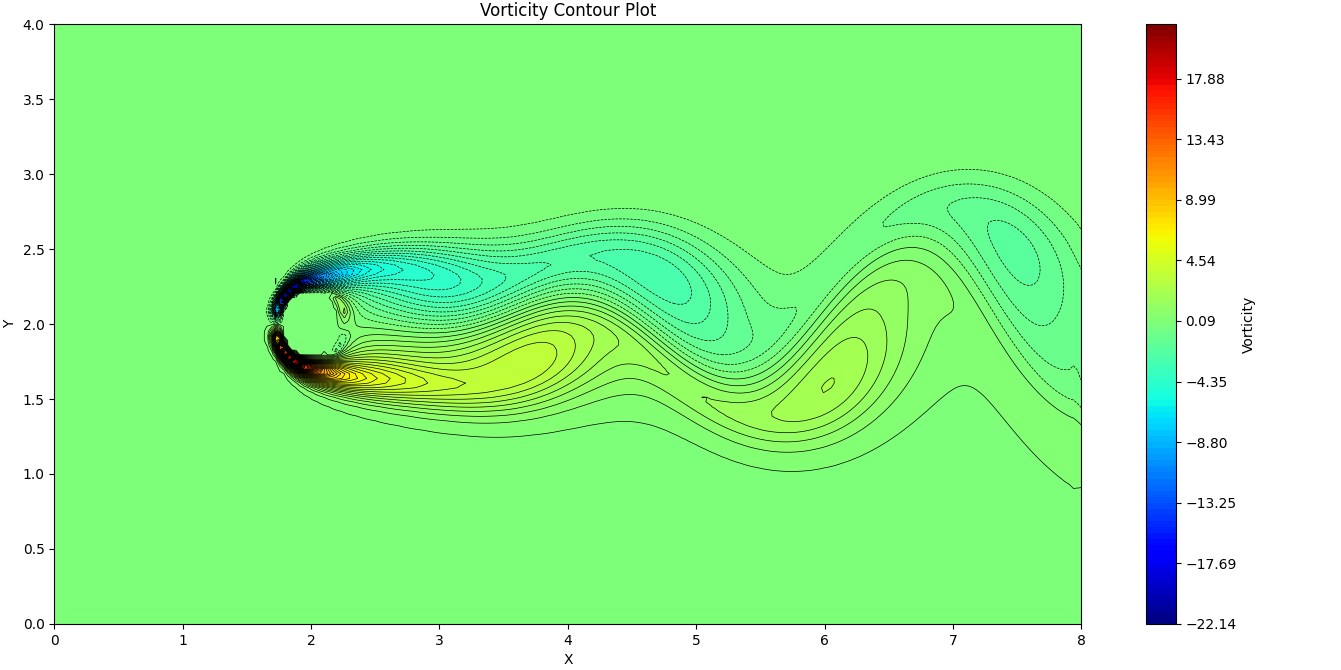
\includegraphics[width=0.3\linewidth]{figure/N32_Re150_8x4_t50/vor_N32_Re150_8x4_t50.jpg}
    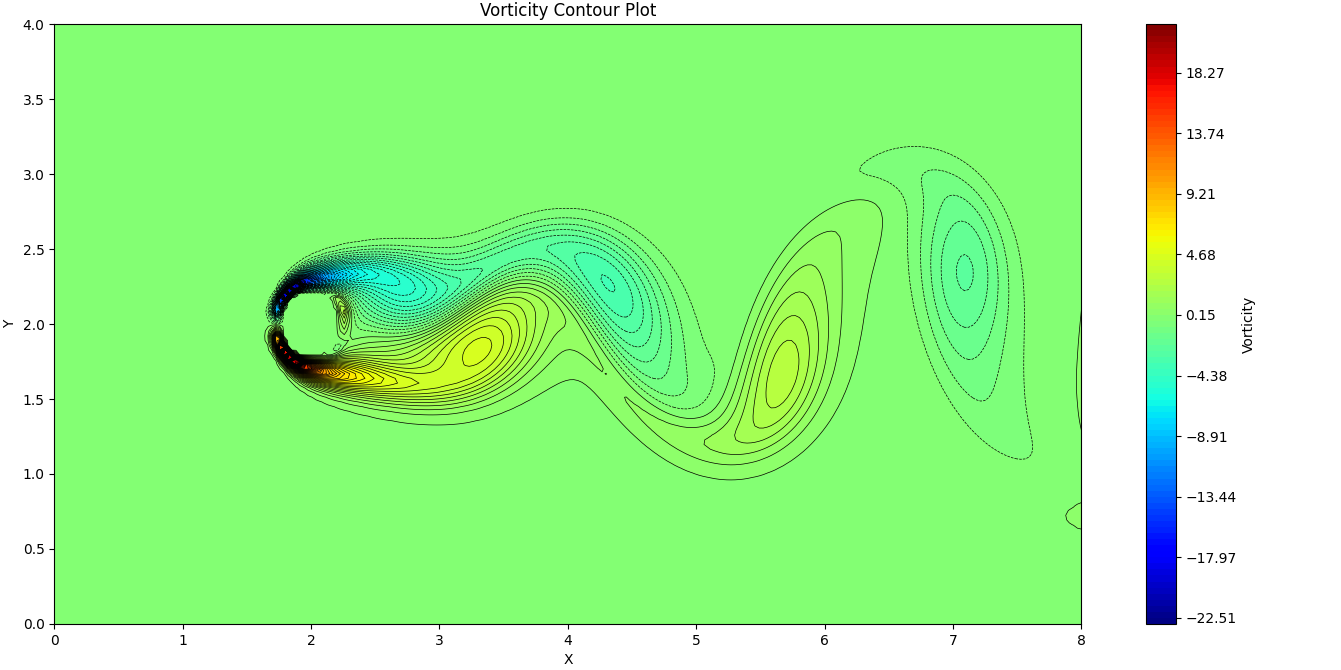
\includegraphics[width=0.3\linewidth]{figure/N32_Re150_8x4_t100/vor_N32_Re150_8x4_t100.jpg}
    \caption{Vorticity at t=10 (left), t=50 (middle), t=100s (right)}
\end{figure}


\begin{figure}[H]
    \centering
    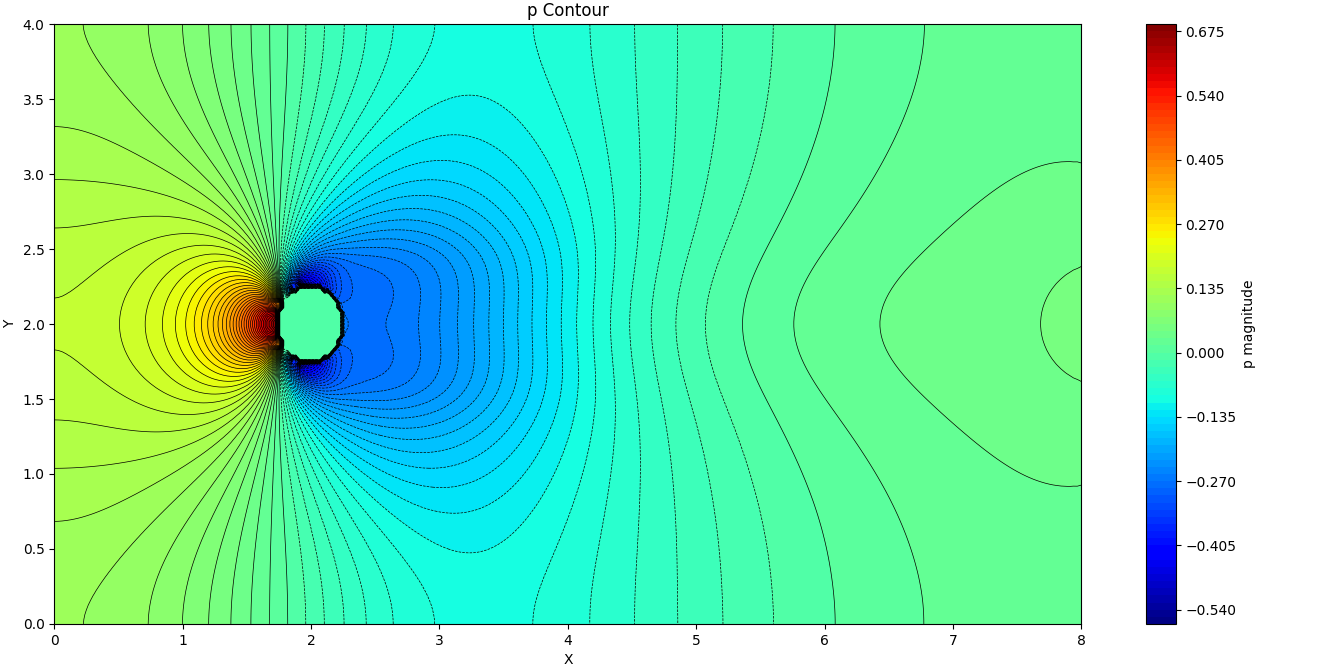
\includegraphics[width=0.3\linewidth]{figure/N32_Re150_8x4_t10/p_N32_Re150_8x4_t10.jpg}
    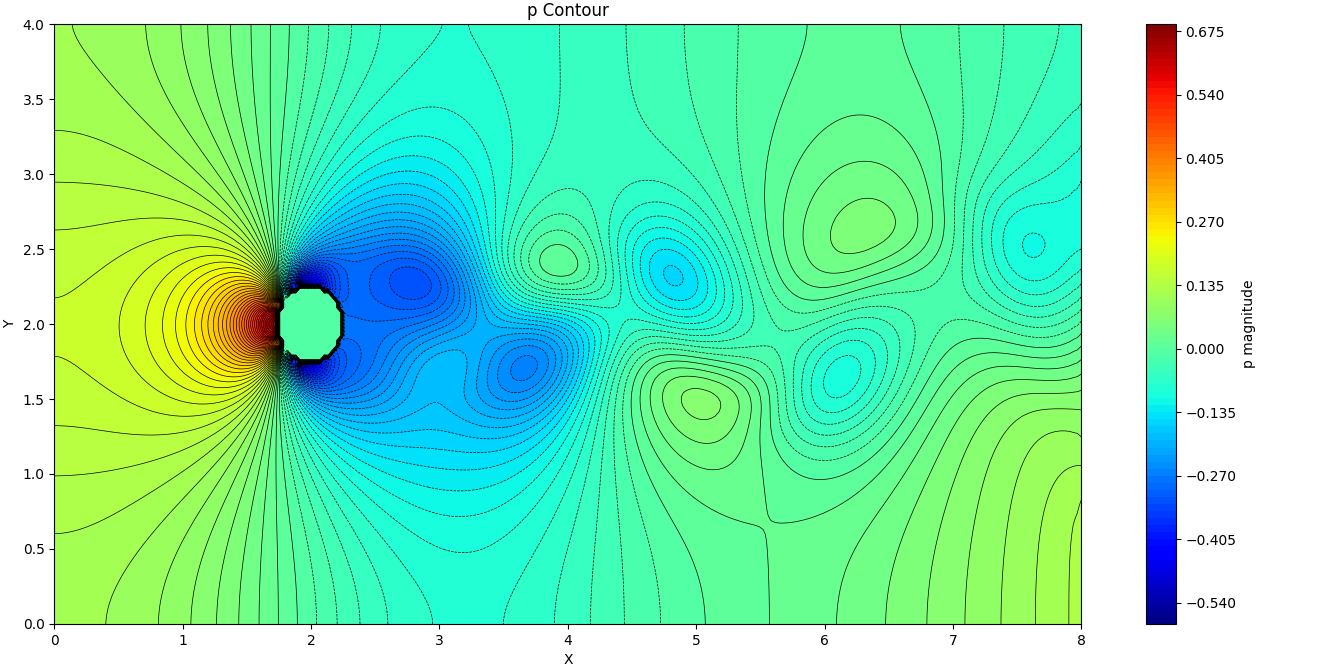
\includegraphics[width=0.3\linewidth]{figure/N32_Re150_8x4_t50/p_N32_Re150_8x4_t50.jpg}
    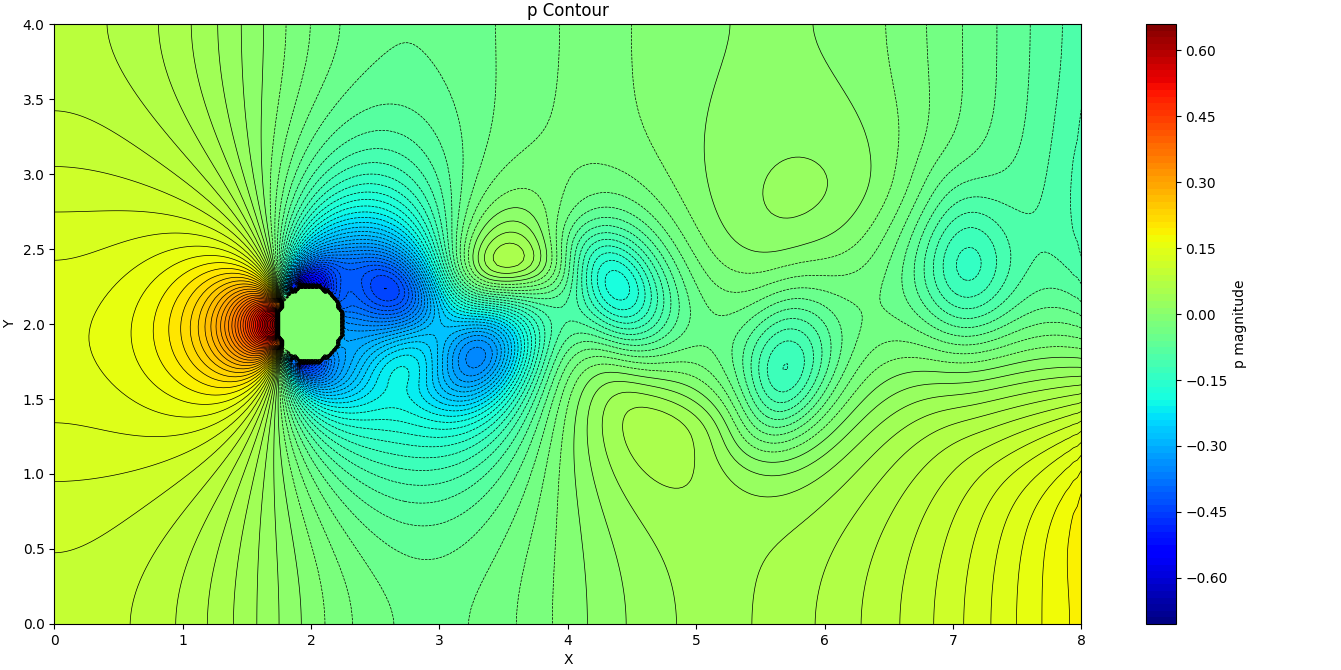
\includegraphics[width=0.3\linewidth]{figure/N32_Re150_8x4_t100/p_N32_Re150_8x4_t100.jpg}
    \caption{Pressure at t=10 (left), t=50 (middle), t=100s (right)}
\end{figure}

Here we put the result among time together. Where it exhibit clearly, that the appearance of vortex shedding is the result of revolution of vortex due to the circular cylinder. 

From streamline plots, pressure disturbance, to vorticity maps, we could observe the evolution from initial flow around the cylinder to the distinct formation of a Kármán vortex street. From t=10 seconds to t=100 seconds, the pressure and vorticity maps reveal changes in the intensity and positioning of these vortices.








\subsection{Re=150 Result Value and Comparison}



\subsubsection{Drag ($c_D$) and Lift ($c_L$) coefficient)}

For large time scale, we sampling 1 second once, the result is showing below:

\begin{figure}[H]
    \centering
    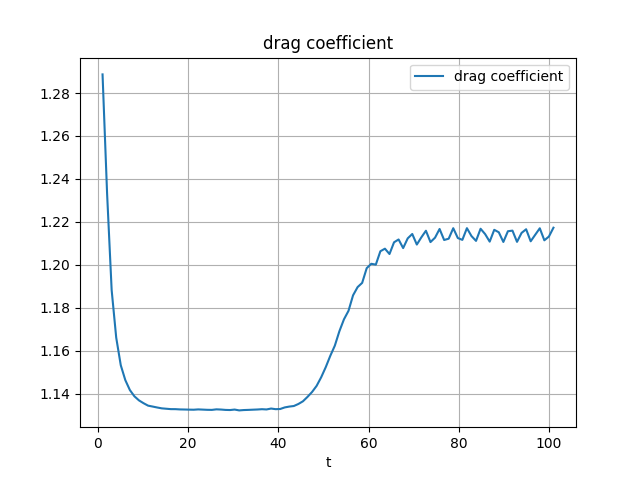
\includegraphics[width=0.45\linewidth]{figure/Analysis/N32_Re150_8x4/cd_largetime.jpg}
    \caption{$c_D$ among long time}
\end{figure}

Based on this figure, we could find the flow become steady after t=70. To increase our result's accuracy, we sampling around t=100 and t=110, sampling 0.01s once. The result is showing below: 








\begin{figure}[H]
    \centering
    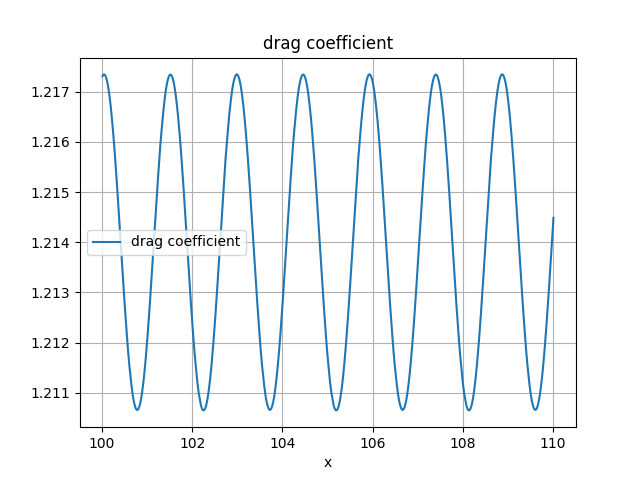
\includegraphics[width=0.45\linewidth]{figure/Analysis/N32_Re150_8x4/cd_N32_Re150_8x4.jpg}
    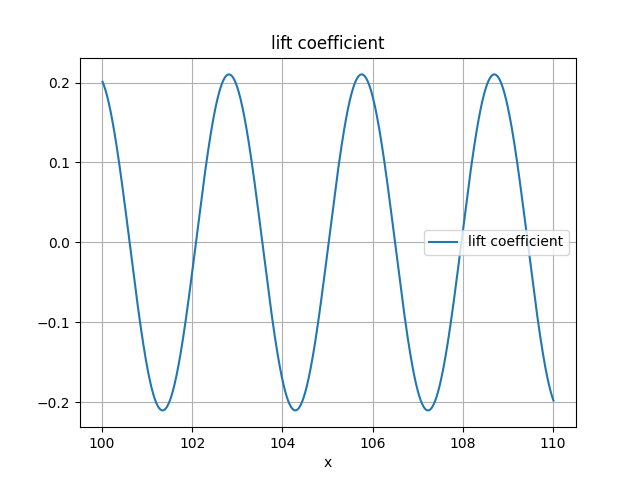
\includegraphics[width=0.45\linewidth]{figure/Analysis/N32_Re150_8x4/cl_N32_Re150_8x4.jpg}
    \caption{$c_L$ and $c_D$ among time}
\end{figure}


We could get the mean drag coefficient ($c_D$):
$$c_D = 1.212$$

Also, we could get lift coefficient ($c_D$):

$$c_L = 0 \pm 0.21$$


\subsubsection{Vortex Shedding frequency}

By sampling the result of drag and lift coefficient ($c_D$ and $c_L$), and using Fast Fourier Transform (FFT), we could get the vortex shedding frequency:
$$f = 0.34$$

Based on that, we could calculate Strouhal number ($St$):

$$St = \frac{f D}{U} = 0.17 $$


\subsubsection{Result value compare with literature}

According to Norberg (2003)\cite{NORBERG200357}, the relationship of $St$ number with $Re$ is shown below:

\begin{figure}[H]
    \centering
    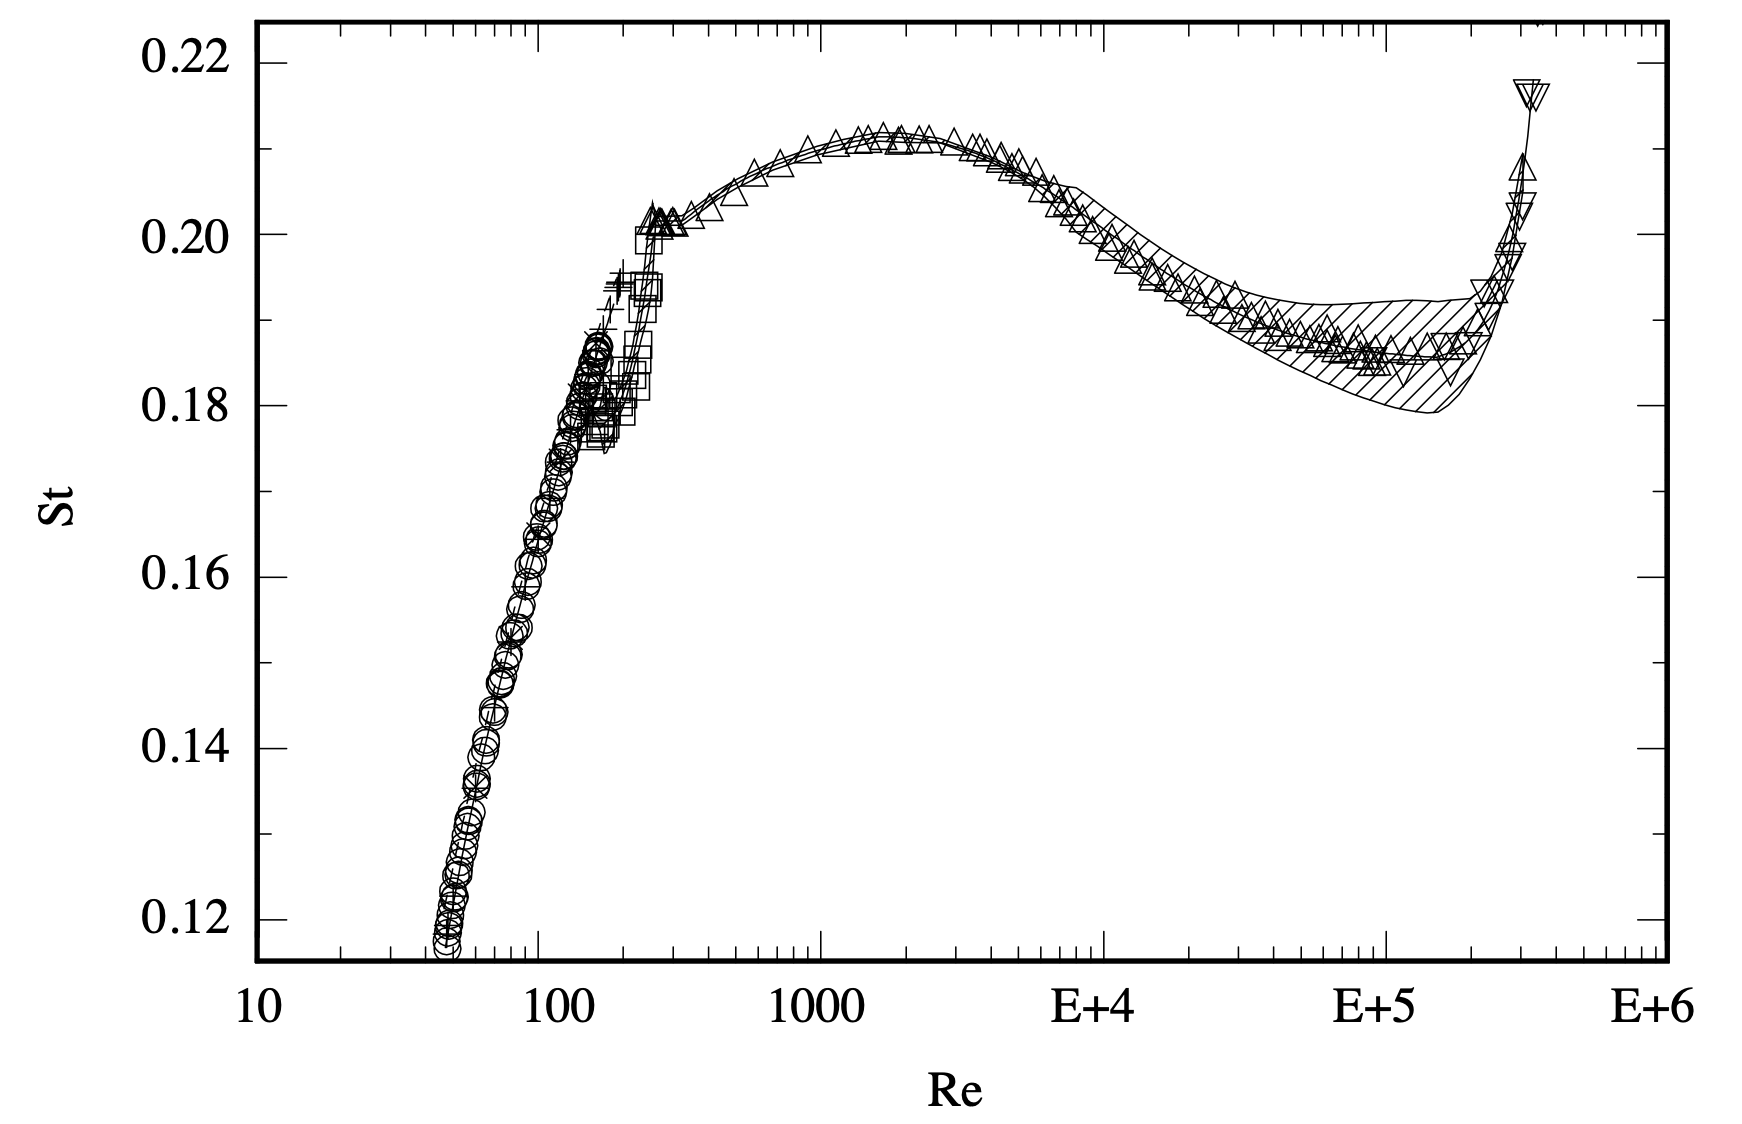
\includegraphics[width=0.6\linewidth]{figure/Literature/Lit-Re_St.jpg}
    \caption{$St$ number with $Re$ (Norberg, 2003\cite{NORBERG200357})}
\end{figure}

As our result shown $St$ number is 0.166 at $Re$=150, we could say our result matched. The more detailed result is from appendix of Norberg's review (2003)\cite{NORBERG200357}:

From Re in range of (47,190):
$$
St = 0.2663 - \frac{1.019}{\sqrt{Re}}
$$

Which shows $St = 0.183$ at $Re=150$, which is also closed to our result.\\



We also compared with Qu (2013)\cite{QU2013347}, where shows $St=0.184$, and $c_{Dp}=1.02$. Compare with our $c_D=1.21$, shows our result may not exactly accurate at calculating drag coefficient.


The total comparison table is showing below:
\begin{table}[ht]
\centering
\caption{Result comparison with Qu(2003)\cite{QU2013347}}
\begin{tabular}{c|ccc}
\toprule
Re=150 & $c_{D_p}$ & $c_L$ & $St$ \\
\midrule
Result & 1.212 & $0 \pm 0.21$ & 0.17 \\
Qu\cite{QU2013347} & 1.02 & 0.35 & 0.184 \\
\bottomrule
\end{tabular}
\end{table}





























%%%%%%%%%%%%%%%%%%%%%%%%%%%%%%%%%%%%%%%%%%%%%%%%%%%%%%%%%%
%%%%%%%%%%%%%%%%%%%%%%%%%%%%%%%%%%%%%%%%%%%%%%%%%%%%%%%%%%
%%%%%%%%%%%%%%%%%%%%%%%%%%%%%%%%%%%%%%%%%%%%%%%%%%%%%%%%%%

\newpage
\section{Influence of Domain Size: $ 8 \times 4 $ VS. $ 8 \times 2 $}
\subsection{Result Comparison among time }

To examine the influence of grid size, we narrow our domain at y-axis, make our domain from $ 8 \times 4 $to $ 8 \times 2$.


\subsubsection{t=50 and t=100 comparison}

The following figures shown below is the vorticity and velocity contour of $ 8 \times 2 $(upper) and $ 8 \times 4$(lower):
\begin{figure}[H]
    \centering
    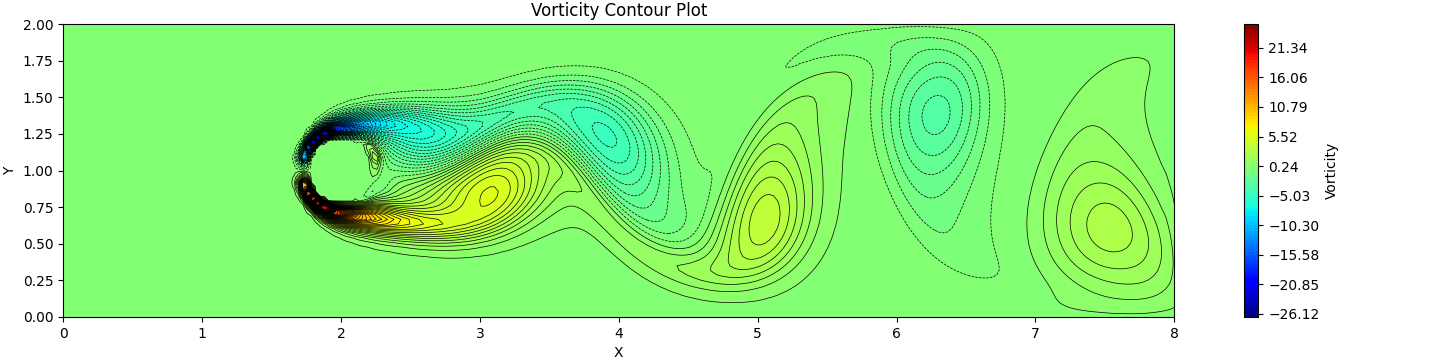
\includegraphics[width=0.6\linewidth]{figure/N32_Re150_8x2_t50/vor_N32_Re150_8x2_t50.jpg}
    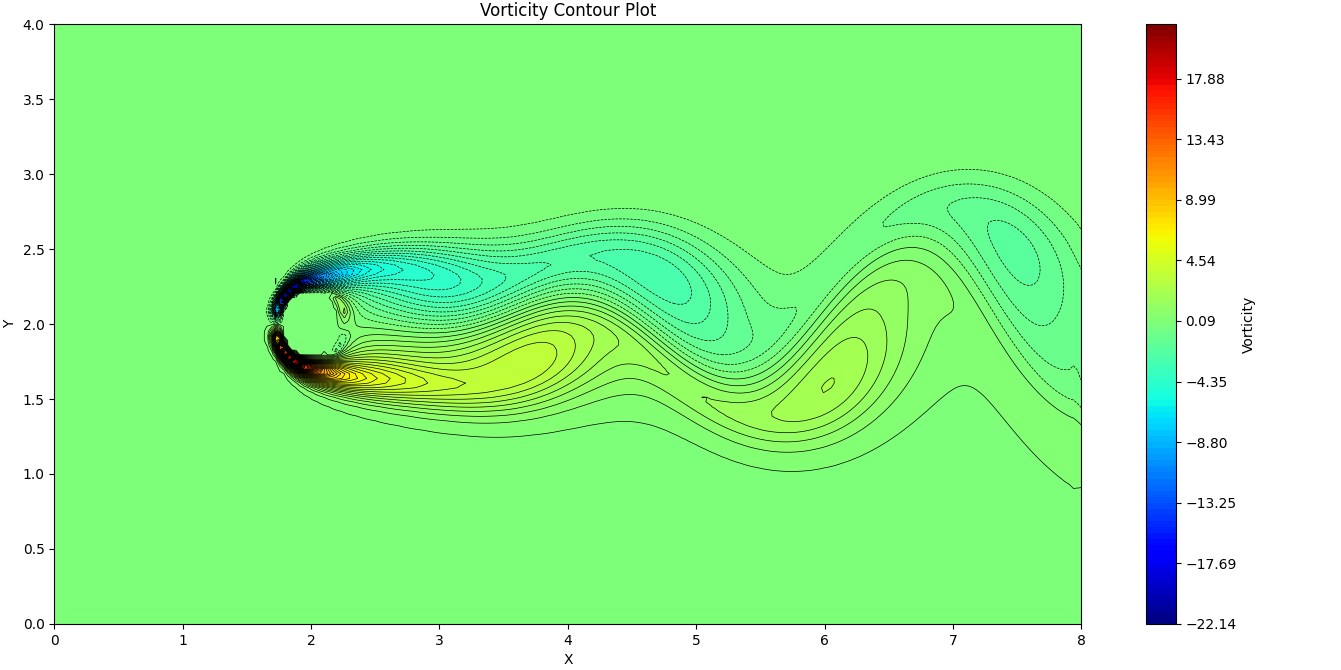
\includegraphics[width=0.6\linewidth]{figure/N32_Re150_8x4_t50/vor_N32_Re150_8x4_t50.jpg}
    \caption{Vorticity at t=50}
\end{figure}

We could find as the domain has been narrowed, the evolution of the flow seems been accelerated, which shows voticies shedding out of cylinder at t=50, domain size $ 8 \times 2$, but still only starting to been disturbed t=50, domain size $ 8 \times 4$. 


\begin{figure}[H]
    \centering
    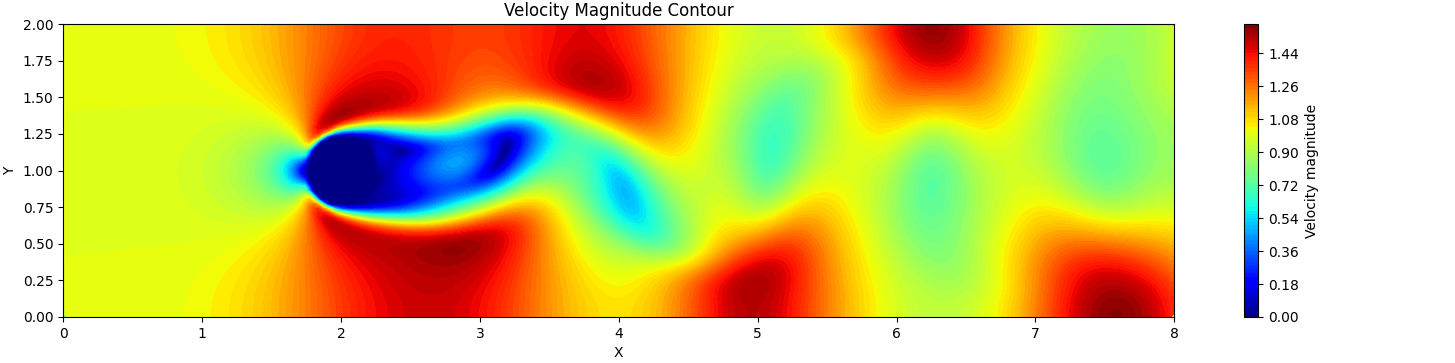
\includegraphics[width=0.6\linewidth]{figure/N32_Re150_8x2_t50/v_N32_Re150_8x2_t50.jpg}
    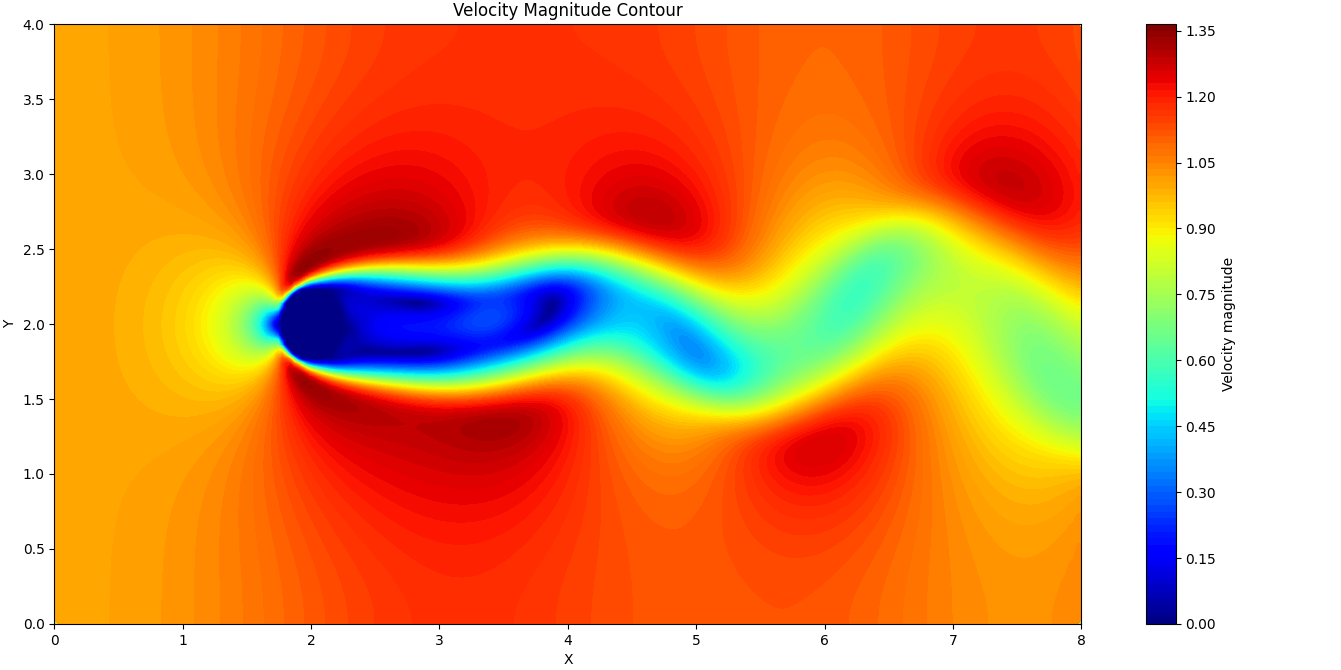
\includegraphics[width=0.6\linewidth]{figure/N32_Re150_8x4_t50/v_N32_Re150_8x4_t50.jpg}
    \caption{Velocity at t=50}
\end{figure}

We could find the domain $ 8 \times 2$ is not enough for the flow simulation, where its boundary is too close, where the vortices touched the boundary. The flow evolution been speed up, where you can see the vortex shedding.


\subsection{Drag ($c_D$) and Lift ($c_L$) coefficient)}

\begin{figure}[H]
    \centering
    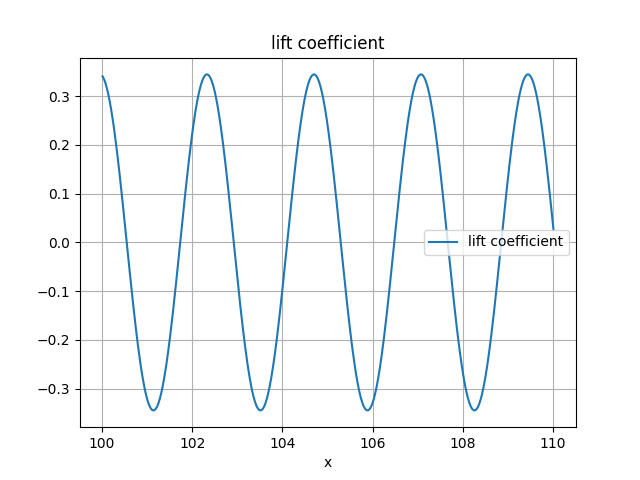
\includegraphics[width=0.45\linewidth]{figure/Analysis/N32_Re150_8x2/cl_N32_Re150_8x2.jpg}
    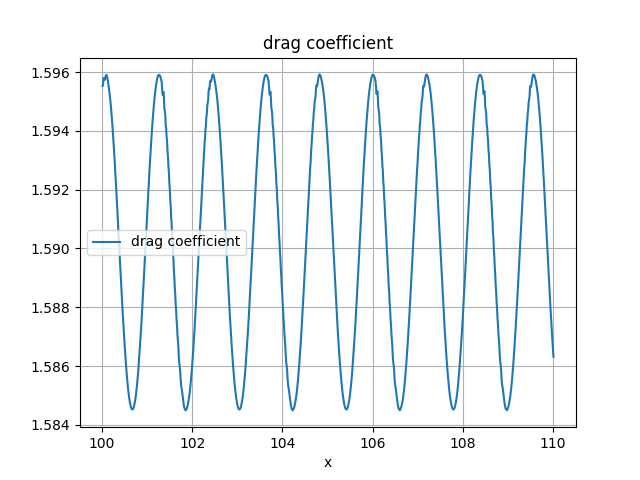
\includegraphics[width=0.45\linewidth]{figure/Analysis/N32_Re150_8x2/cd_N32_Re150_8x2.jpg}
    \caption{$c_L$ and $c_D$ among time}
\end{figure}

We could get the mean drag coefficient ($c_D$):
$$c_D\vert_{8 \times 2} = 1.588$$


\subsubsection{Vortex Shedding frequency}

By sampling the result of drag and lift coefficient ($c_D$ and $c_L$), and using Fast Fourier Transform (FFT), we could get the vortex shedding frequency:
$$f\vert_{8 \times 2} = 0.4$$

Based on that, we could calculate Strouhal number ($St$):

$$St\vert_{8 \times 2} = \frac{f D}{U}\vert_{8 \times 2} = 0.2 $$


\subsection{Comparison of domain size $8 \times 4$ with $8 \times 2$}

We could compare our narrow domain ($8 \times 2$) with our result shown in the previous chapter:

\begin{table}[ht]
\centering
\caption{Result comparison of domain size's effect}
\begin{tabular}{c|ccc}
\toprule
Domain Size & $c_D$ & $c_L$ & $St$ \\
\midrule
$8 \times 4$ & 1.212 & $0 \pm 0.21$ & 0.17 \\
$8 \times 2$ & 1.588 & $0 \pm 0.35$ & 0.2 \\
\bottomrule
\end{tabular}
\end{table}

We could find, after we narrowed the domain size, the result value ($c_D$ and $c_L$) become larger, which may because as we narrowed the domain size, the vortex become much easier to touch the side boundary of the domain, and been mirrored back as we use the symmetric boundary condition. This may cause the flow developed much more faster. 

















%%%%%%%%%%%%%%%%%%%%%%%%%%%%%%%%%%%%%%%%%%%%%%%%%%%%%%%%%%
%%%%%%%%%%%%%%%%%%%%%%%%%%%%%%%%%%%%%%%%%%%%%%%%%%%%%%%%%%
%%%%%%%%%%%%%%%%%%%%%%%%%%%%%%%%%%%%%%%%%%%%%%%%%%%%%%%%%%
\newpage
\section{Influence of Grid Resolution: $\Delta$=1/32 VS. $\Delta$=1/16}


To examine how the grid resolution could influence our result, we use the coarse grid $\Delta$=1/16. 


\subsection{$\Delta$=1/32 VS. $\Delta$=1/16 at different time }

The result shown below is $\Delta$ =1/16 (left), and $\Delta$=32 (right). Form the $\Delta$=1/16 figures, we could find this kind of grid is coarse, where we could easily observe the ``stairs" at the edge of the circle. 

\subsubsection{t=50}
\begin{figure}[H]
    \centering
    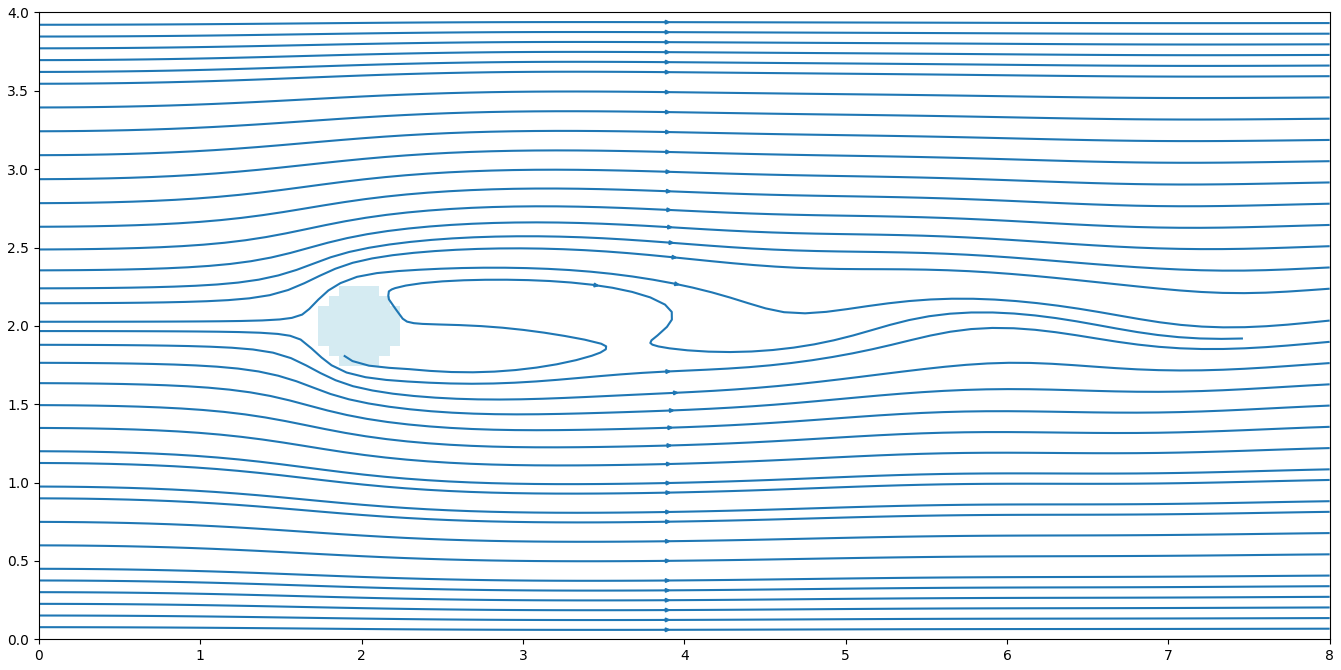
\includegraphics[width=0.45\linewidth]{figure/N16_Re150_8x4_t50/stline_N16_Re150_8x4_t50.jpg}
    \includegraphics[width=0.45\linewidth]{figure/N32_Re150_8x4_t50/stline_N32_Re150_8x4_t50.jpg}
    \caption{Streamline of $\Delta$=1/16 (left), $\Delta$=1/32 (Right) }
\end{figure}

Based on the streamline and velocity contour comparison of the $\Delta$=1/16 with $\Delta$=1/32, we could notice that the flow's development seems been slowed down at $\Delta$=1/16 grid, that the flow is still not been hugely disturbed at t=50 $\Delta$=1/16, but for $\Delta$=1/32 result at t=50, is already starting to show the oscillation.


\begin{figure}[H]
    \centering
    \includegraphics[width=0.45\linewidth]{figure/N16_Re150_8x4_t50/v_N16_Re150_8x4_t50.jpg}
    \includegraphics[width=0.45\linewidth]{figure/N32_Re150_8x4_t50/v_N32_Re150_8x4_t50.jpg}
    \caption{Velocity of $\Delta$=1/16 (left), $\Delta$=1/32 (Right) }
\end{figure}



\begin{figure}[H]
    \centering
    \includegraphics[width=0.45\linewidth]{figure/N16_Re150_8x4_t50/vor_N16_Re150_8x4_t50.jpg}
    \includegraphics[width=0.45\linewidth]{figure/N32_Re150_8x4_t50/vor_N32_Re150_8x4_t50.jpg}
    \caption{Vorticity of $\Delta$=1/16 (left), $\Delta$=1/32 (Right) }
\end{figure}

The similar result showned in the vorticity and pressure contour, where the flow is much un-disturbed at of $\Delta$=1/16.

\begin{figure}[H]
    \centering
    \includegraphics[width=0.45\linewidth]{figure/N16_Re150_8x4_t50/p_N16_Re150_8x4_t50.jpg}
    \includegraphics[width=0.45\linewidth]{figure/N32_Re150_8x4_t50/p_N32_Re150_8x4_t50.jpg}
    \caption{Pressure of $\Delta$=1/16 (left), $\Delta$=1/32 (Right)}
\end{figure}

Based on the comparison of the different grid resolution, we could find that the flow evolution seems been slowed down as the grid become coarse. This may due to the added numerical viscosity at coarse grid. 


\subsubsection{t=100}
\begin{figure}[H]
    \centering
    \includegraphics[width=0.45\linewidth]{figure/N16_Re150_8x4_t100/stline_N16_Re150_8x4_t100.jpg}
    \includegraphics[width=0.45\linewidth]{figure/N32_Re150_8x4_t100/stline_N32_Re150_8x4_t100.jpg}
    \caption{Streamline of $\Delta$=1/16 (left), $\Delta$=1/32 (Right) }
\end{figure}

\begin{figure}[H]
    \centering
    \includegraphics[width=0.45\linewidth]{figure/N16_Re150_8x4_t100/v_N16_Re150_8x4_t100.jpg}
    \includegraphics[width=0.45\linewidth]{figure/N32_Re150_8x4_t100/v_N32_Re150_8x4_t100.jpg}
    \caption{Velocity of $\Delta$=1/16 (left), $\Delta$=1/32 (Right) }
\end{figure}



\begin{figure}[H]
    \centering
    \includegraphics[width=0.45\linewidth]{figure/N16_Re150_8x4_t100/vor_N16_Re150_8x4_t100.jpg}
    \includegraphics[width=0.45\linewidth]{figure/N32_Re150_8x4_t100/vor_N32_Re150_8x4_t100.jpg}
    \caption{Vorticity of $\Delta$=1/16 (left), $\Delta$=1/32 (Right) }
\end{figure}

\begin{figure}[H]
    \centering
    \includegraphics[width=0.45\linewidth]{figure/N16_Re150_8x4_t100/p_N16_Re150_8x4_t100.jpg}
    \includegraphics[width=0.45\linewidth]{figure/N32_Re150_8x4_t100/p_N32_Re150_8x4_t100.jpg}
    \caption{Pressure of $\Delta$=1/16 (left), $\Delta$=1/32 (Right)}
\end{figure}

Based on the result, we could get the conclusion: The narrow domain could accelerate the flow evolution, and the coarse grid could slow down the flow development among time due to the large numerical viscosity.




\subsection{Drag ($c_D$) and Lift ($c_L$) coefficient)}

\begin{figure}[H]
    \centering
    \includegraphics[width=0.45\linewidth]{figure/Analysis/N16Re150_8x4/cl_N16Re150_8x4.jpg}
    \includegraphics[width=0.45\linewidth]{figure/Analysis/N16Re150_8x4/cd_N16Re150_8x4.jpg}
    \caption{$c_L$ and $c_D$ among time}
\end{figure}

We could get the mean drag coefficient ($c_D$):
$$c_D = 1.22$$


\subsubsection{Vortex Shedding frequency}

By sampling the result of drag and lift coefficient ($c_D$ and $c_L$), and using Fast Fourier Transform (FFT), we could get the vortex shedding frequency:
$$f = 0.3$$

Based on that, we could calculate Strouhal number ($St$):

$$St = \frac{f D}{U} = 0.15 $$

\subsection{Result comparison of grid resolution: 1/32 and 1/16}

\begin{table}[H]
\centering
\caption{Result comparison of grid resolution effect}
\begin{tabular}{c|ccc}
\toprule
Grid Size & $c_D$ & $c_L$ & $St$ \\
\midrule
1/32 & 1.212 & $0 \pm 0.21$ & 0.17 \\
1/16 & 1.22 & $0 \pm 0.18 $ & 0.15 \\
\bottomrule
\end{tabular}
\end{table}

We could find that as we use the coarse grid, the result ($c_L$) is little bit smaller. As we also could notice that the flow developed much more slower than the finer grid, which may because as we use coarse grid, we make the fluid cannot catch the number of small part's of the circle cylinder's influence of the flow, and make the numerical viscosity much higher, which could influence the result.




 



%%%%%%%%%%%%%%%%%%%%%%%%%%%%%%%%%%%%%%%%%%%%%%%%%%%%%%%%%%%%%%%%%%%%%%%
%%%%%%%%%%%%%%%%%%%%%%%%%%%%%%%%%%%%%%%%%%%%%%%%%%%%%%%%%%%%%%%%%%%%%%%
%%%%%%%%%%%%%%%%%%%%%%%%%%%%%%%%%%%%%%%%%%%%%%%%%%%%%%%%%%%%%%%%%%%%%%%



\newpage
\section{Re=300 Result}
To observe Re number effect for circular cylinder cross-sectional flow, we simulate the Re=300 case, and compare with Re=150 result which is shown at the previous section. The result is showing below:

\subsection{Re=300 VS. Re=150 at different time }
The result of Re=300 compared with Re=150 result is showing below:

\subsubsection{t=50}
\begin{figure}[H]
    \centering
    \includegraphics[width=0.45\linewidth]{figure/N32_Re300_8x4_t50/stline_N32_Re300_8x4_t50.jpg}
    \includegraphics[width=0.45\linewidth]{figure/N32_Re150_8x4_t50/stline_N32_Re150_8x4_t50.jpg}
    \caption{Streamline for Re=300 (left), Re=150 (right)}
\end{figure}

We could notice for the higher Re number, the development for the flow seems been speed up at Re=300, which could already observe vortex shedding at t=50, where for Re=150 the flow is just stating to oscillate.

\begin{figure}[H]
    \centering
    \includegraphics[width=0.45\linewidth]{figure/N32_Re300_8x4_t50/v_N32_Re300_8x4_t50.jpg}
    \includegraphics[width=0.45\linewidth]{figure/N32_Re150_8x4_t50/v_N32_Re150_8x4_t50.jpg}
    \caption{Velocity for Re=300 (left), Re=150 (right) }
\end{figure}



\begin{figure}[H]
    \centering
    \includegraphics[width=0.45\linewidth]{figure/N32_Re300_8x4_t50/vor_N32_Re300_8x4_t50.jpg}
    \includegraphics[width=0.45\linewidth]{figure/N32_Re150_8x4_t50/vor_N32_Re150_8x4_t50.jpg}
    \caption{Vorticity for Re=300 (left), Re=150 (right) }
\end{figure}

\begin{figure}[H]
    \centering
    \includegraphics[width=0.45\linewidth]{figure/N32_Re300_8x4_t50/p_N32_Re300_8x4_t50.jpg}
    \includegraphics[width=0.45\linewidth]{figure/N32_Re150_8x4_t50/p_N32_Re150_8x4_t50.jpg}
    \caption{Pressure for Re=300 (left), Re=150 (right)}
\end{figure}


\subsubsection{t=100}
\begin{figure}[H]
    \centering
    \includegraphics[width=0.45\linewidth]{figure/N32_Re300_8x4_t100/stline_N32_Re300_8x4_t100.jpg}
    \includegraphics[width=0.45\linewidth]{figure/N32_Re150_8x4_t100/stline_N32_Re150_8x4_t100.jpg}
    \caption{Streamline for Re=300 (left), Re=150 (right) }
\end{figure}

\begin{figure}[H]
    \centering
    \includegraphics[width=0.45\linewidth]{figure/N32_Re300_8x4_t100/v_N32_Re300_8x4_t100.jpg}
    \includegraphics[width=0.45\linewidth]{figure/N32_Re150_8x4_t100/v_N32_Re150_8x4_t100.jpg}
    \caption{Pressure for Re=300 (left), Re=150 (right) }
\end{figure}



\begin{figure}[H]
    \centering
    \includegraphics[width=0.45\linewidth]{figure/N32_Re300_8x4_t100/vor_N32_Re300_8x4_t100.jpg}
    \includegraphics[width=0.45\linewidth]{figure/N32_Re150_8x4_t100/vor_N32_Re150_8x4_t100.jpg}
    \caption{Vorticity for Re=300 (left), Re=150 (right) }
\end{figure}

\begin{figure}[H]
    \centering
    \includegraphics[width=0.45\linewidth]{figure/N32_Re300_8x4_t100/p_N32_Re300_8x4_t100.jpg}
    \includegraphics[width=0.45\linewidth]{figure/N32_Re150_8x4_t100/p_N32_Re150_8x4_t100.jpg}
    \caption{Pressure for Re=300 (left), Re=150 (right)}
\end{figure}



\subsection{Re=300 Result Value and Comparison}

\subsubsection{Drag ($c_D$) and Lift ($c_L$) coefficient}

\begin{figure}[H]
    \centering
    \includegraphics[width=0.45\linewidth]{figure/Analysis/N32_Re300_8x4/cd_N32_Re300_8x4.jpg}
    \includegraphics[width=0.45\linewidth]{figure/Analysis/N32_Re300_8x4/cl_N32_Re300_8x4.jpg}
    \caption{$c_L$ and $c_D$ among time}
\end{figure}

We could get the mean drag coefficient ($c_D$):
$$c_D = 1.21$$


Also, we could get lift coefficient ($c_D$):

$$c_L = 0 \pm 0.46$$



\subsubsection{Vortex Shedding frequency}

By sampling the result of drag and lift coefficient ($c_D$ and $c_L$), and using Fast Fourier Transform (FFT), we could get the vortex shedding frequency:
$$f = 0.4$$

Based on that, we could calculate Strouhal number ($St$):

$$St = \frac{f D}{U} = 0.2 $$


\subsubsection{Result value compare with literature}

According to Franke(1990)\cite{FRANKE1990237}, the result of $St$ at $Re=300$: $St = 0.205$, where our result is $St = 0.2$, which is close.

\begin{table}[ht]
\centering
\caption{Result comparison with literature}
\begin{tabular}{c|ccc}
\toprule
 & $c_{D_p}$ & $c_{L_p}$ & $St$ \\
\midrule
Re=300 & 1.21 & $0 \pm 0.46$ & 0.2 \\
Franke\cite{FRANKE1990237} & 1.11 &  $0 \pm 0.77$ & 0.205 \\
\bottomrule
\end{tabular}
\end{table}
























%%%%%%%%%%%%%%%%%%%%%%%%%%%%%%%%%%%%%%%%%%%%%%%%%%%%%%%%%%%%%%%%%%%%%%%
%%%%%%%%%%%%%%%%%%%%%%%%%%%%%%%%%%%%%%%%%%%%%%%%%%%%%%%%%%%%%%%%%%%%%%%
%%%%%%%%%%%%%%%%%%%%%%%%%%%%%%%%%%%%%%%%%%%%%%%%%%%%%%%%%%%%%%%%%%%%%%%


\newpage
\section{Re=1000 Result}
To observe Re number effect for circular cylinder cross-sectional flow, we simulate the Re=1000 case, and compare with Re=150 result which is shown at the previous section. The result is showing below:

\subsection{Re=1000 VS. Re=150 at different time }
The following figures shows Re=1000 result (left), and Re=150 result (right):


\subsubsection{t=50}
\begin{figure}[H]
    \centering
    \includegraphics[width=0.45\linewidth]{figure/N32_Re1000_8x4_t50/stline_N32_Re1000_8x4_t50.jpg}
    \includegraphics[width=0.45\linewidth]{figure/N32_Re150_8x4_t50/stline_N32_Re150_8x4_t50.jpg}
    \caption{Streamline for Re=300 (left), Re=150 (right)}
\end{figure}

Based on the streamline and velocity contour, we could clearly observe vortex shedding from circular cylinder at Re=1000, t=50. But for Re=150, t=50, we could find the flow is only starting to been disturbed, but not shown vortex shedding yet.

\begin{figure}[H]
    \centering
    \includegraphics[width=0.45\linewidth]{figure/N32_Re1000_8x4_t50/v_N32_Re1000_8x4_t50.jpg}
    \includegraphics[width=0.45\linewidth]{figure/N32_Re150_8x4_t50/v_N32_Re150_8x4_t50.jpg}
    \caption{Velocity contour for Re=300 (left), Re=150 (right) }
\end{figure}




\begin{figure}[H]
    \centering
    \includegraphics[width=0.45\linewidth]{figure/N32_Re1000_8x4_t50/vor_N32_Re1000_8x4_t50.jpg}
    \includegraphics[width=0.45\linewidth]{figure/N32_Re150_8x4_t50/vor_N32_Re150_8x4_t50.jpg}
    \caption{Vorticity for Re=300 (left), Re=150 (right) }
\end{figure}

From vorticity and pressure contour, we could get the similar observation: the vortex shedding is already shown up at Re=1000, but not clearly shown up at Re=150, t=50.

\begin{figure}[H]
    \centering
    \includegraphics[width=0.45\linewidth]{figure/N32_Re1000_8x4_t50/p_N32_Re1000_8x4_t50.jpg}
    \includegraphics[width=0.45\linewidth]{figure/N32_Re150_8x4_t50/p_N32_Re150_8x4_t50.jpg}
    \caption{Pressure for Re=300 (left), Re=150 (right)}
\end{figure}


\subsubsection{t=100}
\begin{figure}[H]
    \centering
    \includegraphics[width=0.45\linewidth]{figure/N32_Re1000_8x4_t100/stline_N32_Re1000_8x4_t100.jpg}
    \includegraphics[width=0.45\linewidth]{figure/N32_Re150_8x4_t100/stline_N32_Re150_8x4_t100.jpg}
    \caption{Streamline for Re=300 (left), Re=150 (right) }
\end{figure}

We could also notice that for Re=1000, the vortices kindly lying up, which neatly aligned after the circular cylinder.

\begin{figure}[H]
    \centering
    \includegraphics[width=0.45\linewidth]{figure/N32_Re1000_8x4_t100/v_N32_Re1000_8x4_t100.jpg}
    \includegraphics[width=0.45\linewidth]{figure/N32_Re150_8x4_t100/v_N32_Re150_8x4_t100.jpg}
    \caption{Velocity for Re=300 (left), Re=150 (right) }
\end{figure}


The similar result shown at vorticity and pressure contour, which we could see there voticies and pressure extremum points arranged neatly.




\begin{figure}[H]
    \centering
    \includegraphics[width=0.45\linewidth]{figure/N32_Re1000_8x4_t100/vor_N32_Re1000_8x4_t100.jpg}
    \includegraphics[width=0.45\linewidth]{figure/N32_Re150_8x4_t100/vor_N32_Re150_8x4_t100.jpg}
    \caption{Vorticity for Re=300 (left), Re=150 (right) }
\end{figure}

\begin{figure}[H]
    \centering
    \includegraphics[width=0.45\linewidth]{figure/N32_Re1000_8x4_t100/p_N32_Re1000_8x4_t100.jpg}
    \includegraphics[width=0.45\linewidth]{figure/N32_Re150_8x4_t100/p_N32_Re150_8x4_t100.jpg}
    \caption{Pressure for Re=300 (left), Re=150 (right)}
\end{figure}

















\subsection{Re=1000 Result Value and Comparison}

\subsubsection{Drag ($c_D$) and Lift ($c_L$) coefficient}

\begin{figure}[H]
    \centering
    \includegraphics[width=0.45\linewidth]{figure/Analysis/N32_Re1000_8x4/cl_N32_Re1000_8x4.jpg}
    \includegraphics[width=0.45\linewidth]{figure/Analysis/N32_Re1000_8x4/cd_N32_Re1000_8x4.jpg}
    \caption{$c_L$ and $c_D$ among time}
\end{figure}


We could get the mean drag coefficient ($c_D$):
$$c_D = 1.36$$


Also, we could get lift coefficient ($c_D$):

$$c_L = 0 \pm 0.97$$



\subsubsection{Vortex Shedding frequency}

By sampling the result of drag and lift coefficient ($c_D$ and $c_L$), and using Fast Fourier Transform (FFT), we could get the vortex shedding frequency:
$$f = 0.4$$

Based on that, we could calculate Strouhal number ($St$):

$$St = \frac{f D}{U} = 0.2 $$


\subsubsection{Result value compare with literature}

According to Qu(2003)\cite{QU2013347}, the result of $St$ at $Re=1000$: $St = 0.2365$, where our result is $St = 0.2$, could say our result is close.

\begin{table}[ht]
\centering
\caption{Comparison with Qu(2003)\cite{QU2013347} result}
\begin{tabular}{c|ccc}
\toprule
 & $c_{D_p}$ & $c_{L_p}$ & $St$ \\
\midrule
Re=1000 & 1.36 & $0 \pm 0.97$ & 0.2 \\
Qu\cite{QU2013347} & 1.34 &  $0 \pm 1.30$ & 0.236 \\
\bottomrule
\end{tabular}
\end{table}


\subsection{Comparison and discussion of Re number effect on result}
\subsubsection{$C_D$ and $C_L $ comparison}

\begin{table}[H]
\centering
\caption{Result comparison of Re effect}
\begin{tabular}{c|ccc}
\toprule
Re & $c_{D_p}$ & $c_{L_p}$ & $St$ \\
\midrule
Re=150 & 1.212 & $0 \pm 0.21$ & 0.17 \\
Re=300 & 1.21 & $0 \pm 0.46$ & 0.2 \\
Re=1000 & 1.36 & $0 \pm 0.97$ & 0.2 \\
\bottomrule
\end{tabular}
\end{table}

Based on the comparison, we could find for higher Re, the $c_L$'s maximum value will be higher, and $c_D$ may have the same effect but not obviously in our result.




\subsubsection{Comparison among time}

To have a more comprehensive understanding of the Re number's effect of our result, we put Re=1000 (left), Re=300 (middle), and Re=150 (right)'s figures together to check how Re could influence the simulation outcome:\\

\noindent \textbf{t=50:}

\begin{figure}[H]
    \centering
    \includegraphics[width=0.3\linewidth]{figure/N32_Re1000_8x4_t50/stline_N32_Re1000_8x4_t50.jpg}
    \includegraphics[width=0.3\linewidth]{figure/N32_Re300_8x4_t50/stline_N32_Re300_8x4_t50.jpg}
    \includegraphics[width=0.3\linewidth]{figure/N32_Re150_8x4_t50/stline_N32_Re150_8x4_t50.jpg}
    \caption{Streamline for Re=1000 (left), Re=300 (middle), Re=150 (right)}
\end{figure}

Based on the streamline and velocity contour comparison of Re=1000, Re=300, and Re=150, we could find that as Re become higher, the vortices evolution seems been speed up, and its become aligned up at Re become higher


\begin{figure}[H]
    \centering
    \includegraphics[width=0.3\linewidth]{figure/N32_Re1000_8x4_t50/v_N32_Re1000_8x4_t50.jpg}
    \includegraphics[width=0.3\linewidth]{figure/N32_Re300_8x4_t50/v_N32_Re300_8x4_t50.jpg}
    \includegraphics[width=0.3\linewidth]{figure/N32_Re150_8x4_t50/v_N32_Re150_8x4_t50.jpg}
    \caption{Velocity contour for Re=1000 (left), Re=300 (middle), Re=150 (right) }
\end{figure}



\begin{figure}[H]
    \centering
    \includegraphics[width=0.3\linewidth]{figure/N32_Re1000_8x4_t50/vor_N32_Re1000_8x4_t50.jpg}
    \includegraphics[width=0.3\linewidth]{figure/N32_Re300_8x4_t50/vor_N32_Re300_8x4_t50.jpg}
    \includegraphics[width=0.3\linewidth]{figure/N32_Re150_8x4_t50/vor_N32_Re150_8x4_t50.jpg}
    \caption{Vorticity for Re=1000 (left), Re=300 (middle), Re=150 (right) }
\end{figure}


\begin{figure}[H]
    \centering
    \includegraphics[width=0.3\linewidth]{figure/N32_Re1000_8x4_t50/p_N32_Re1000_8x4_t50.jpg}
    \includegraphics[width=0.3\linewidth]{figure/N32_Re300_8x4_t50/p_N32_Re300_8x4_t50.jpg}
    \includegraphics[width=0.3\linewidth]{figure/N32_Re150_8x4_t50/p_N32_Re150_8x4_t50.jpg}
    \caption{Pressure for Re=1000 (left), Re=300 (middle), Re=150 (right)}
\end{figure}



\noindent \textbf{t=100:}
\begin{figure}[H]
    \centering
    \includegraphics[width=0.3\linewidth]{figure/N32_Re1000_8x4_t100/stline_N32_Re1000_8x4_t100.jpg}
    \includegraphics[width=0.3\linewidth]{figure/N32_Re300_8x4_t100/stline_N32_Re300_8x4_t100.jpg}
    \includegraphics[width=0.3\linewidth]{figure/N32_Re150_8x4_t100/stline_N32_Re150_8x4_t100.jpg}
    \caption{Streamline for Re=1000 (left), Re=300 (middle), Re=150 (right) }
\end{figure}

\begin{figure}[H]
    \centering
    \includegraphics[width=0.3\linewidth]{figure/N32_Re1000_8x4_t100/v_N32_Re1000_8x4_t100.jpg}
    \includegraphics[width=0.3\linewidth]{figure/N32_Re300_8x4_t100/v_N32_Re300_8x4_t100.jpg}
    \includegraphics[width=0.3\linewidth]{figure/N32_Re150_8x4_t100/v_N32_Re150_8x4_t100.jpg}
    \caption{Velocity for Re=1000 (left), Re=300 (middle), Re=150 (right) }
\end{figure}



\begin{figure}[H]
    \centering
    \includegraphics[width=0.3\linewidth]{figure/N32_Re1000_8x4_t100/vor_N32_Re1000_8x4_t100.jpg}
    \includegraphics[width=0.3\linewidth]{figure/N32_Re300_8x4_t100/vor_N32_Re300_8x4_t100.jpg}
    \includegraphics[width=0.3\linewidth]{figure/N32_Re150_8x4_t100/vor_N32_Re150_8x4_t100.jpg}
    \caption{Vorticity for Re=1000 (left), Re=300 (middle), Re=150 (right)}
\end{figure}

\begin{figure}[H]
    \centering
    \includegraphics[width=0.3\linewidth]{figure/N32_Re1000_8x4_t100/p_N32_Re1000_8x4_t100.jpg}
    \includegraphics[width=0.3\linewidth]{figure/N32_Re300_8x4_t100/p_N32_Re300_8x4_t100.jpg}
    \includegraphics[width=0.3\linewidth]{figure/N32_Re150_8x4_t100/p_N32_Re150_8x4_t100.jpg}
    \caption{Pressure for Re=1000 (left), Re=300 (middle), Re=150 (right)}
\end{figure}



Based on the Re result comparison among time, we could find that as we increase Re number, the flow develop become much faster, which make the vortex shedding show up earlier. 

We also could observe that as the Re number increase, the vortices begin to align neatly after the circular cylinder.









%%%%%%%%%%%%%%%%%%%%%%%%%%%%%%%%%%%%%%%%%%%%%%%%%%%%%%%%%%%%%%%%%%%%%%%
%%%%%%%%%%%%%%%%%%%%%%%%%%%%%%%%%%%%%%%%%%%%%%%%%%%%%%%%%%%%%%%%%%%%%%%
%%%%%%%%%%%%%%%%%%%%%%%%%%%%%%%%%%%%%%%%%%%%%%%%%%%%%%%%%%%%%%%%%%%%%%%


\newpage
\section{Re=300, Elliptic cylinder}


In this section, we replaced our circular cylinder with 3:1 elliptic cylinder, and its angle of attack at 30 degrees, and Re=300. 

\subsection{Elliptic Setting}

Based on the requirement shown above, our ellipse control equation as follows:

$$
\frac{((x-x_0)\cos{\theta_0}+(y-y_0)\sin{\theta_0})^2}{a^2}+
\frac{(-(x-x_0)\sin{\theta_0}+(y-y_0)\cos{\theta_0})^2}{b^2} = 1
$$

Where, $\theta_0$ is the angle of the ellipse rotation. In our case, $\theta_0 = -30$ to full fill our angle-of-attack requirement.\\

The domain setting is as follows:

\begin{figure}[H]
    \centering
    \includegraphics[width=0.6\linewidth]{figure/Solver and Stting/Ellipse_Setting.jpg}
    \caption{Domain and boundary setting for Elliptic cylinder}
\end{figure}

The Domain setting as shown above. The key parameters as follows:
\begin{itemize}
    \item \textbf{Ly=4, Lx=8}: Width and Length of the domain
    \item \textbf{Ellipse Center}: the location of Elliptic cylinder center=$(\frac{Lx}{4}, \frac{Ly}{2})$
    \item  \textbf{a=0.6, b=0.3}: The long, and short axis of the ellipse.

    \item \textbf{Inlet}: $u=1, v=0, \frac{\partial p}{\partial x}=0$
    \item \textbf{Side}: $\frac{\partial u}{\partial y}=0, \frac{\partial v}{\partial y}=0, 
    \frac{\partial p}{\partial y}=0$
    \item \textbf{Outlet}: $\frac{\partial u}{\partial x}=0, \frac{\partial v}{\partial x}=0, 
    \frac{\partial p}{\partial x}=0$
\end{itemize}






\subsection{t=50 and t=100}
By setting the parameters as the chapter shown before, we now exhibit the result of t=50 and t=100 as follows:

\begin{figure}[H]
    \centering
    \includegraphics[width=0.45\linewidth]{figure/Ellip_N32_Re300_8x4_t50/stline_Ellip_N32_Re300_8x4_t50.jpg}
    \includegraphics[width=0.45\linewidth]{figure/Ellip_N32_Re300_8x4_t100/stline_Ellip_N32_Re300_8x4_t100.jpg}
    \caption{Streamline at t=50 (left), t=100s (right)}
\end{figure}

Based on streamline and velocity, we could see there is a vortex generated at the east south point of the ellipse, and the cortex generated at this point then shed off from ellipse. We could observe the vortices shedding is already shown up at t=50.

\begin{figure}[H]
    \centering
    \includegraphics[width=0.45\linewidth]{figure/Ellip_N32_Re300_8x4_t50/v_Ellip_N32_Re300_8x4_t50.jpg}
    \includegraphics[width=0.45\linewidth]{figure/Ellip_N32_Re300_8x4_t100/v_Ellip_N32_Re300_8x4_t100.jpg}
    \caption{Velocity at t=50 (left), t=100s (right)}
\end{figure}



\begin{figure}[H]
    \centering
    \includegraphics[width=0.45\linewidth]{figure/Ellip_N32_Re300_8x4_t50/vor_Ellip_N32_Re300_8x4_t50.jpg}
    \includegraphics[width=0.45\linewidth]{figure/Ellip_N32_Re300_8x4_t100/vor_Ellip_N32_Re300_8x4_t100.jpg}
    \caption{Vorticity at t=50 (left), t=100s (right)}
\end{figure}



\begin{figure}[H]
    \centering
    \includegraphics[width=0.45\linewidth]{figure/Ellip_N32_Re300_8x4_t50/p_Ellip_N32_Re300_8x4_t50.jpg}
    \includegraphics[width=0.45\linewidth]{figure/Ellip_N32_Re300_8x4_t100/p_Ellip_N32_Re300_8x4_t100.jpg}
    \caption{Pressure at t=50 (left), t=100s (right)}
\end{figure}







\subsubsection{Comparison among time (t=5, 10, 50, 100)}
As we could already observe vortex shedding showing up at t=50, and t=100, we here plot the result among more time steps:

\begin{figure}[H]
    \centering
    \includegraphics[width=0.23\linewidth]{figure/Ellip_N32_Re300_8x4_t05/stline_Ellip_N32_Re300_8x4_t05.jpg}
    \includegraphics[width=0.23\linewidth]{figure/Ellip_N32_Re300_8x4_t10/stline_Ellip_N32_Re300_8x4_t10.jpg}
    \includegraphics[width=0.23\linewidth]{figure/Ellip_N32_Re300_8x4_t50/stline_Ellip_N32_Re300_8x4_t50.jpg}
    \includegraphics[width=0.23\linewidth]{figure/Ellip_N32_Re300_8x4_t100/stline_Ellip_N32_Re300_8x4_t100.jpg}
    \caption{Streamline at t=5 (left), t=10 (middle left), t=50 (middle right) t=100s (right)}
\end{figure}

Based on the time comparison for more time scale figures, we could see how the vortex generated and shed off from ellipse. Based on the pressure contour, we could see there is main pressure low point shown at the ease south side of the ellipse. 



\begin{figure}[H]
    \centering
    \includegraphics[width=0.23\linewidth]{figure/Ellip_N32_Re300_8x4_t05/v_Ellip_N32_Re300_8x4_t05.jpg}
    \includegraphics[width=0.23\linewidth]{figure/Ellip_N32_Re300_8x4_t10/v_Ellip_N32_Re300_8x4_t10.jpg}
    \includegraphics[width=0.23\linewidth]{figure/Ellip_N32_Re300_8x4_t50/v_Ellip_N32_Re300_8x4_t50.jpg}
    \includegraphics[width=0.23\linewidth]{figure/Ellip_N32_Re300_8x4_t100/v_Ellip_N32_Re300_8x4_t100.jpg}
    \caption{Velocity at t=5 (left), t=10 (middle left), t=50 (middle right) t=100s (right)}
\end{figure}



\begin{figure}[H]
    \centering
    \includegraphics[width=0.23\linewidth]{figure/Ellip_N32_Re300_8x4_t05/vor_Ellip_N32_Re300_8x4_t05.jpg}
    \includegraphics[width=0.23\linewidth]{figure/Ellip_N32_Re300_8x4_t10/vor_Ellip_N32_Re300_8x4_t10.jpg}
    \includegraphics[width=0.23\linewidth]{figure/Ellip_N32_Re300_8x4_t50/vor_Ellip_N32_Re300_8x4_t50.jpg}
    \includegraphics[width=0.23\linewidth]{figure/Ellip_N32_Re300_8x4_t100/vor_Ellip_N32_Re300_8x4_t100.jpg}
    \caption{Vorticity at t=5 (left), t=10 (middle left), t=50 (middle right) t=100s (right)}
\end{figure}

% The result for velocity magnitude and pressure disturbance is similar, where at t=10, flow shows symmetric pattern along y-center, but not anymore at t=50.

\begin{figure}[H]
    \centering
    \includegraphics[width=0.23\linewidth]{figure/Ellip_N32_Re300_8x4_t05/p_Ellip_N32_Re300_8x4_t05.jpg}
    \includegraphics[width=0.23\linewidth]{figure/Ellip_N32_Re300_8x4_t10/p_Ellip_N32_Re300_8x4_t10.jpg}
    \includegraphics[width=0.23\linewidth]{figure/Ellip_N32_Re300_8x4_t50/p_Ellip_N32_Re300_8x4_t50.jpg}
    \includegraphics[width=0.23\linewidth]{figure/Ellip_N32_Re300_8x4_t100/p_Ellip_N32_Re300_8x4_t100.jpg}
    \caption{Pressure at t=5 (left), t=10 (middle left), t=50 (middle right) t=100s (right)}
\end{figure}

At t=50 and t=100, we could see the vortex aligned up after the ellipse.








\subsection{Elliptic Result Value and Comparison}

\subsubsection{Drag ($c_D$) and Lift ($c_L$) coefficient}

\begin{figure}[H]
    \centering
    \includegraphics[width=0.45\linewidth]{figure/Analysis/Ellipt_N32_Re300_8x4/cl_Ellipt_N32_Re300_8x4.jpg}
    \includegraphics[width=0.45\linewidth]{figure/Analysis/Ellipt_N32_Re300_8x4/cd_Ellipt_N32_Re300_8x4.jpg}
    \caption{$c_L$ and $c_D$ among time}
\end{figure}

We could get the mean drag coefficient ($c_L$):
$$c_L = 0.81$$


Also, we could get mean lift coefficient ($c_D$):

$$c_D = 0.76$$



\subsubsection{Vortex Shedding frequency}

By sampling the result of drag and lift coefficient ($c_D$ and $c_L$), and using Fast Fourier Transform (FFT), we could get the vortex shedding frequency:
$$f = 0.2$$

Based on that, we could calculate Strouhal number ($St$):

$$St = \frac{f D}{U} = 0.36 $$























%%%%%%%%%%%%%%%%%%%%%%%%%%%%%%%%%%%%%%%%%%%%%%%%%%%%%%%%%%%%%%%%%%%%%%%
%%%%%%%%%%%%%%%%%%%%%%%%%%%%%%%%%%%%%%%%%%%%%%%%%%%%%%%%%%%%%%%%%%%%%%%
%%%%%%%%%%%%%%%%%%%%%%%%%%%%%%%%%%%%%%%%%%%%%%%%%%%%%%%%%%%%%%%%%%%%%%%




\newpage
\section{Discussion and Conclusion}

\subsection{Review of the result}
In this project, we discritized N-S equation and applied to our N-S solver. The solver perform well in uniform flow and channel flow, which its result matched therodially result. 
We applied our solver to the circular cylinder cross sectional flow, it shows vortex shedding after several time steps.

\subsubsection{Re=150, domain size= $8 \times 4$, grid resolution $\Delta = 1/32$}
% \noindent \textbf{Re=150, domain size= $8 \times 4$, grid resolution $\Delta = 1/32$}:\\
We compared our result for different time scale. We could observe the vortex generating among time, and  dislodged from circular cylinder. Among time, the flow been disturbed significantly.


\subsubsection{Re=150, domain size= $8 \times 2$, grid resolution $\Delta = 1/32$}
In order to explore how could the domain size influence our result, we simulate the same flow in domain size $8 \times 2$, which is \textbf{Re=150, domain size= $8 \times 2$, grid resolution $\Delta = 1/32$} case:\\

For this case, we compared our result with $8 \times 4$ case, we could find that the vortex evolution been speed up, which could see the vortex shedding appear early, and been squeezed as the vortex touched the sides of the domain.


\subsubsection{Re=150, domain size= $8 \times 4$, grid resolution $\Delta = 1/16$}
In order to explore how could grid resolution can influence our result, we also tried a coarse grid. We let grid size $\Delta = 1/16$, which is \textbf{Re=150, domain size= $8 \times 4$, grid resolution $\Delta = 1/16$} case:\\

In this case, we could find that the flow evolution seems been slowed down, compare with $\Delta = 1/32$ grid resolution. This may due to the numerical viscosity which been added by our discretization, and as the grid become coarser, the viscosity increased, make the vortex hard to shed.


\subsubsection{Re=300, domain size= $8 \times 4$, grid resolution $\Delta = 1/32$}
To discuss Re number's influence of the result of the flow, we use Re=300 and compare with Re=150 case:\\

In this case, we could find the vortex generated earlier, and the flow become more disturbed
for Re=300, compare with Re=150 case at the same time scale. The vortex shedding appearance seems been speed up.

\subsubsection{Re=1000, domain size= $8 \times 4$, grid resolution $\Delta = 1/32$}
To discuss Re number's influence of the result of the flow more, we also tried Re=1000 case\\

The vortex generating and shedding out of the circular cylinder seems been more speed up, and we also could notice that vortex lying up, neatly aligned after the circular cylinder.

We put Re=1000, Re=300, and Re=150 cases together to get a more comprehensive understanding of the vortex shedding. We could find as Re number become higher, the vortex shedding appear earlier, and the vortex aligned up more neatly.

\subsubsection{Elliptic Case: Re=300, domain size= $8 \times 4$, grid resolution $\Delta = 1/32$}

In this case, we replaced our circular cylinder to the elliptic cylinder, and we could observe the vortex been generated at the lower right side of the cylinder, and among time, the vortex become more exhibit.



\subsection{Result and Observation}

\begin{table}[H]
\centering
\label{tab:comparison}
\begin{tabular}{c|c|c|c|c|c|c|c |c}
\toprule
& \textbf{Re} & \textbf{Re} & \textbf{Re} & \textbf{8x2} & \textbf{1/6} & Re  & Re & Re \\ 
& \textbf{150} & \textbf{300} & \textbf{1000} & \textbf{Narrow} & \textbf{Coarse} & 150  & 300& 1000 \\ 
&  & &  & \textbf{Domain} & \textbf{Grid} & \cite{QU2013347} & \cite{FRANKE1990237}& \cite{QU2013347} \\ 
\hline
\textbf{\(C_D\)} & 1.212 & 1.21  &  1.36   & 1.588 & 1.22 & 1.02  & 1.11 & 1.34 \\ 
\textbf{\(C_L\)} & $\pm 0.21$ & $\pm 0.46$ & $\pm 0.97$  & $\pm 0.35$ & $\pm 0.18$ & $\pm 0.35$  & $\pm 0.77$ & $\pm 1.30$\\ 

\textbf{\(St\)} & 0.17 & 0.2 & 0.2  & 0.2 & 0.15 & 0.184  & 0.205 & 0.236 \\ 
\bottomrule
\end{tabular}
\caption{Total Comparison: (Reference: Qu(2003)\cite{QU2013347}, Franke(1990)\cite{FRANKE1990237})}
\end{table}


Based the observation and comparison, we could find that for small domain, the flow evolution is much faster, to make the vortex shedding show up earlier, increase Re number have the similar effect. Decrease grid resolution, in the other hand, have the opposite effect, which could slow down the vortex generation, however, it could not prevent vortex generation.









\subsection{Discussion}
Based the observation and comparison, we could find that for small domain, the vortex shedding occur earlier, which may because of the the flow been squeezed, and as we use the symmetric boundary condition at the side of domain ($frac{\partial}{\partial n}$=0), the flow touched the side of domain and been mirrored back, make the flow layering together, make the vortex show up earlier.\\

We found increase Re number have the similar effect, where Re number been increase, the flow become much easier to be disturbed, and make the vortex generate earlier.\\

Based on the comparison of coarse grid comparison, we found as we use large grid size (poor resolution), the flow evolution become slower. This may because of the grid size make the flow harder to been disturbed by the cylinder, and make the wave easier to transfer to the edge of the domain, make the flow evolution much slower. However, coarse grid cannot prevent the vortex shedding, as we finally observed the vortex shedding after the circular cylinder.





\subsection{Conclusion}
In this project, we discretized the Navier-Stokes equations to build and validate an N-S solver, which was then applied to flow simulations around circular and elliptical cylinders. At a Reynolds number (Re) of 150, we compared our results with existing literature and confirmed that our results are both sound and reliable.\\

To analyze how domain size, grid resolution, and Reynolds number influence our numerical results, we adjusted the domain size from $8 \times 4$ to $8 \times 2$, and modified the grid resolution from $\Delta = 1/32$ to $\Delta = 1/16$. We also explored the outcomes at Re = 300 and Re = 1000.\\

We observed that smaller domain sizes accelerated the flow evolution, leading to earlier vortex shedding. This phenomenon is likely due to the constrained flow being compressed, which accelerates disturbances within the fluid. Similarly, increasing the Reynolds number enhances the flow's susceptibility to disturbances, thereby promoting earlier vortex formation. These effects are consistent across different configurations, confirming the impact of domain size and Reynolds number on the observed fluid dynamics.\\

Conversely, reducing the grid resolution had an inhibitory effect on the rate of flow evolution. A coarser grid introduces greater numerical viscosity due to our discretization method, which damps fluid disturbances and delays the development of vortices. However, even with reduced resolution, vortex shedding cannot be entirely prevented, only delayed. This indicates that while grid resolution influences the speed of flow disturbances, it does not alter the fundamental dynamics responsible for vortex shedding.































\bibliographystyle{plain}
\bibliography{ref}
% \cite{NORBERG200357}
% \cite{FRANKE1990237}
% \cite{QU2013347}




%%%%%%%%%%%%%%%%%%%%%%%%%%%%%%%%%%%%%%%%%%%%%%%%%%%%%%%%%%%%%%%
%%%%%%%%%%%%%%%%%%%%%%%%%%%%%%%%%%%%%%%%%%%%%%%%%%%%%%%%%%%%%%%
%%%%%%%%%%%%%%%%%%%%%%%%%%%%%%%%%%%%%%%%%%%%%%%%%%%%%%%%%%%%%%%
\newpage
\section*{Appendix}
% 在目录中添加Appendix
\addcontentsline{toc}{section}{Appendix}


The Project Data and python scripts are located at:
\href{https://github.com/ZHBALEX/Numerical-CFD/tree/cd4f80f52957a564282440dbf4f327c3e4eac02a/CFD%20Projects/CFD_Final_Circular_Cylinder_Cross-Flow}{Github link (click this)}

\noindent \textbf{Our basic Solver code is showing below:}
\begin{scriptsize}
\begin{lstlisting}[language=python,caption={N-S Cylinder Solver}]
import numpy as np
import matplotlib.pyplot as plt
plt.ioff() 
import copy
import re

class mesher:
    def __init__(self, data):
        self.Lx = data["Lx"]
        self.Ly = data["Ly"]
        self.dxy = data["dx"]

    def parameter_grid(self): # generate large grid 
        Field1 = grid_generator( self.Ly,  self.Lx, self.dxy)
        N_rows, N_cols,a = np.shape(Field1)

        # save location y,x in field[j,i,0], 
        for j in range(0, N_rows):
            for i in range(0,N_cols):
                Field1[j,i,0] , Field1[j,i,1] = (j-1/2)*self.dxy, (i-1/2)*self.dxy
        # save fluid(1)/Solid(0) in field[j,i,2]
        Field1[:,:,2] = i_fluid_detector(Field1[:,:,0], Field1[:,:,1], Field1[:,:,2])
        Field1[:,:,3] = 1 - Field1[:,:,2]
        return Field1
    
def grid_generator( y_size,  x_size, grid_size):
        print(1.1)
        Nx , Ny = int(x_size/grid_size), int(y_size/grid_size)
        print(1.2)
        print(Ny,Nx)
        Field = np.full((Ny+2, Nx+2, 4), 0 ,dtype = 'float')
        print(1.3)
        return Field

def i_fluid_detector(field_y, field_x, field):
    N_rows, N_cols = np.shape(field)
    for j in range(0, N_rows):
        for i in range(0, N_cols ):
            result = 0
            result = circle_function(field_y[j,i], field_x[j,i])
            if result < 0:
                field[j,i] = 0
            else:
                field[j,i] = 1
    return field

def circle_function(y,x):
    R= 0.25
    x_c = data['Lx']*1/4
    y_c = data['Ly']*1/2
    result = (x-x_c)**2 + (y-y_c)**2 - R**2
    return result
        
def IBM_uv_coeff_change(c_W, c_E, c_S, c_N, c_P, iF, iS): # iF: ifluid. iS: isolid
        c_P[1:-1,1:-1] = c_P[1:-1,1:-1] -(
            iS[1:-1,:-2]*c_W[1:-1,1:-1] +
            iS[1:-1,2:]*c_E[1:-1,1:-1] +
            iS[:-2,1:-1]*c_S[1:-1,1:-1] +
            iS[2:,1:-1]*c_N[1:-1,1:-1] ) 
        c_W[1:-1,1:-1] = iF[1:-1,:-2] * c_W[1:-1,1:-1]
        c_E[1:-1,1:-1] = iF[1:-1,2:] * c_E[1:-1,1:-1]
        c_S[1:-1,1:-1] = iF[:-2,1:-1] * c_S[1:-1,1:-1]
        c_N[1:-1,1:-1] = iF[2:,1:-1] * c_N[1:-1,1:-1]

        c_P[1:-1,1:-1] = iF[1:-1,1:-1] * c_P[1:-1,1:-1] + iS[1:-1,1:-1]
        c_E[1:-1,1:-1] = Solid__coeff_correct(c_E, iF)
        c_W[1:-1,1:-1] = Solid__coeff_correct(c_W, iF)
        c_N[1:-1,1:-1] = Solid__coeff_correct(c_N, iF)
        c_S[1:-1,1:-1] = Solid__coeff_correct(c_S, iF)
        return c_W, c_E, c_S, c_N, c_P
 

def IBM_p_coeff_change(c_W, c_E, c_S, c_N, c_P, iF, iS): # iF: ifluid. iS: isolid
        c_P[1:-1,1:-1] = c_P[1:-1,1:-1] +(
            iS[1:-1,:-2]*c_W[1:-1,1:-1] +
            iS[1:-1,2:]*c_E[1:-1,1:-1] +
            iS[:-2,1:-1]*c_S[1:-1,1:-1] +
            iS[2:,1:-1]*c_N[1:-1,1:-1] ) 
        c_W[1:-1,1:-1] = iF[1:-1,:-2] * c_W[1:-1,1:-1]
        c_E[1:-1,1:-1] = iF[1:-1,2:] * c_E[1:-1,1:-1]
        c_S[1:-1,1:-1] = iF[:-2,1:-1] * c_S[1:-1,1:-1]
        c_N[1:-1,1:-1] = iF[2:,1:-1] * c_N[1:-1,1:-1]
        
        c_P[1:-1,1:-1] = iF[1:-1,1:-1] * c_P[1:-1,1:-1] + iS[1:-1,1:-1]
        c_E[1:-1,1:-1] = Solid__coeff_correct(c_E, iF)
        c_W[1:-1,1:-1] = Solid__coeff_correct(c_W, iF)
        c_N[1:-1,1:-1] = Solid__coeff_correct(c_N, iF)
        c_S[1:-1,1:-1] = Solid__coeff_correct(c_S, iF)
        return c_W, c_E, c_S, c_N, c_P

def Solid__coeff_correct(C, iF):
        return np.copy(C[1:-1,1:-1] * iF[1:-1,1:-1])

def TDMA(a, b, c, d):  # TDMA Solver, input abcd in same length
    # a[0], c[-1] not been used
    do = d.copy(); ao = a.copy(); bo = b.copy(); co = c.copy()
    N = len(d)
    xo = np.zeros(N)
    for rowi in range(1,N):
        k = ao[rowi]/bo[rowi-1]
        bo[rowi] -= co[rowi-1]*k
        do[rowi] -= do[rowi-1]*k
    xo[N-1] = do[N-1]/bo[N-1]
    for rowi in range(N-2,-1,-1):
        xo[rowi] = (do[rowi]-co[rowi]*xo[rowi+1])/bo[rowi]
    return xo

def general_grid_generator(len_x, Nx, Ny):
    # Creating same size of u, v, U, V
    # where col 0, row 0, row -1, of U not used
    # where row 0, col 0, col -1, of V not used
    initial_Value = 0.01
    dx = len_x/Nx
    grid = np.full((Ny+2, Nx+2), initial_Value)
    grid[0,0] = grid[-1,-1] = grid[-1,0] = grid[0,-1] = np.inf
    u,v,U,V = data_copy(grid, grid, grid, grid)
    p = np.copy(grid)
    return u, v, U, V, p, dx

def data_copy(u, v, U, V):
    return np.copy(u), np.copy(v), np.copy(U), np.copy(V)

def Ghost_BC_p(p_input): # updating ghost point for p based on BC condition
    p = np.copy(p_input)
    p[-1,1:-1] =   p[-2,1:-1] # upper BC
    p[0, 1:-1] =   p[1,1:-1] # bottom BC
    p[1:-1, 0] =   p[1:-1,1] # left BC
    p[1:-1, -1] =  p[1:-1,-2] # right BC
    return p

def Ghost_BC_u(u): # updating ghost point for p based on BC condition
    u[-1,1:-1] =   u[-2,1:-1] # upper BC
    u[0, 1:-1] =   u[1,1:-1] # bottom BC
    u[1:-1, 0] =   2-u[1:-1,1] # left BC
    u[1:-1, -1] =  u[1:-1,-2] # right BC
    u = u[:,:]*iF[:,:]
    return u

def Ghost_BC_v(v): # updating ghost point for p based on BC condition
    v[-1,1:-1] =   -v[-2,1:-1] # upper BC
    v[0, 1:-1] =   -v[1,1:-1] # bottom BC
    v[1:-1, 0] =   -v[1:-1,1] # left BC
    v[1:-1, -1] =   v[1:-1,-2] # right BC
    v = v[:,:]*iF[:,:]
    return v

def UV_BC(U, V, u, iF):
    U[1:-1,1] = 1 # left
    V[1,:] = 0 # bottom
    V[-1,:] = 0 # upper
    U[1:-1,1:-1] = U[1:-1,1:-1] * iF[1:-1,1:-1] 
    U[1:-1,2:]   = U[1:-1,2:]   * iF[1:-1,1:-1] 
    V[1:-1,1:-1] = V[1:-1,1:-1] * iF[1:-1,1:-1] 
    V[2:,1:-1]   = V[2:,1:-1]   * iF[1:-1,1:-1]
    return U,V

def coeff_assemble(rows_cols, a_e, b_e, c_e, e_e, f_e):
    rows, cols = rows_cols[0], rows_cols[1]
    # input elements of abcdef, get line matrix of abcdef
    a = np.full((rows, cols), a_e ) # abc in same length of Ncols of u
    b = np.full((rows, cols), b_e )
    c = np.full((rows, cols), c_e )
    e = np.full((rows, cols), e_e ) # ef in same length of Nrows of u
    f = np.full((rows, cols), f_e )
    a[:,0]= a[:,-1] = c[:,0] = c[:,-1] = 0
    b[:,0] = b[:,-1] = 1
    e[:,-1] =e[:,0] = f[:,-1]= f[:,0]=0
    e[0,:] = e[-1,:] = f[0,:] = f[-1,:] = 0
    a[0,:] = a[-1,:] = c[0,:] = c[-1,:] = 0
    return a,b,c, e,f

def RHS_uv(f, f_old, U, V, U_old, V_old, c0, r): 
    # Update Right Hand Side
    f_P = f[1:-1,1:-1]
    f_W = f[1:-1,:-2]
    f_E = f[1:-1,2:]
    f_S = f[:-2,1:-1]
    f_N = f[2:,1:-1]

    f_P_old = f_old[1:-1,1:-1]
    f_W_old = f_old[1:-1,:-2]
    f_E_old = f_old[1:-1,2:]
    f_S_old = f_old[:-2,1:-1]
    f_N_old = f_old[2:,1:-1]
    convection_new = c0*( U[1:-1,2:] * (f_E + f_P)/2 -
                          U[1:-1,1:-1] * (f_W + f_P)/2 +
                          V[2:,1:-1]  * (f_N + f_P)/2 -
                          V[1:-1,1:-1] * (f_S + f_P)/2 )
    convection_old = c0*( U_old[1:-1,2:] * (f_E_old + f_P_old)/2 -
                          U_old[1:-1,1:-1] * (f_W_old + f_P_old)/2 +
                          V_old[2:,1:-1]  * (f_N_old + f_P_old)/2 -
                          V_old[1:-1,1:-1] * (f_S_old + f_P_old)/2 )
    
    diffusion = f_P + r*(f_E + f_W + f_N + f_S -4*f_P)
    return -3/2*convection_new + 1/2*convection_old + diffusion

def Residual(u, a, b, c, d, e, f):
    return (a[1:-1,1:-1] * u[1:-1,:-2] +
                      b[1:-1,1:-1] * u[1:-1,1:-1] +
                      c[1:-1,1:-1] * u[1:-1,2:] +
                      e[1:-1,1:-1] * u[:-2,1:-1] +
                      f[1:-1,1:-1] * u[2:,1:-1] -
                      d[:,:])

def LineSOR_u(a,b,c,d,e,f, u): 
    # input abcdef, and u, get :D
    # then use TDMA get new u
    # abc is in same size of N_rows of u, ef in same size of N_cols of u
    # ! Input d is LIKE inner field of u, need to cut each line to use !
    u_k = np.copy(u)
    u_k_new = np.copy(u)
    n_rows = np.size(u,0)
    w = 1.3
    D = np.zeros_like(a[1,:])
    Res = 100
    k = 0
    while Res>1e-6:
        u_k = np.copy(u_k_new) 
        for j in range(1,n_rows-1): # the number is based on d, which is (N-1)x(N-1)
            D[1:-1] = d[j-1,:] - e[j,1:-1]*u_k_new[j-1,1:-1] - f[j,1:-1]*u_k_new[j+1,1:-1]
            D[0], D[-1] = 2-u_k_new[j,1], u_k_new[j,-2] # ghost point = ghost point
            u_k_new[j,:] = TDMA(a[j,:],b[j,:],c[j,:],D) # TDMA solve uk each line
            u_k_new[j,1:-1] = u_k[j,1:-1]*(1-w) +u_k_new[j,1:-1]*w # SOR term
        u_k_new = Ghost_BC_u(u_k_new)
        Res = np.max(np.abs(Residual(u_k_new, a, b, c, d, e, f)))
        # print("Res_u=")
        # print(Res) 
        u = np.copy(u_k)
        # print(Residual(u_k_new, a, b, c, d, e, f))
        k+=1
    return u_k_new, k, Res

def LineSOR_v(a,b,c,d,e,f, u): 
    # input abcdef, and u, get D
    # then use TDMA get new u
    # abc is in same size of N_rows of u, ef in same size of N_cols of u
    # ! Input d is LIKE inner field of u, need to cut each line to use !
    u_k = np.copy(u)
    u_k_new = np.copy(u)
    n_rows = np.size(u,0)
    w = 1.3
    D = np.zeros_like(a[1,:])
    Res = 100
    k = 0
    while Res>1e-6:
        u_k = np.copy(u_k_new) 
        for j in range(1,n_rows-1): # the number is based on d, which is (N-1)x(N-1)
            D[1:-1] = d[j-1,:] - e[j,1:-1]*u_k_new[j-1,1:-1] - f[j,1:-1]*u_k_new[j+1,1:-1]
            D[0], D[-1] = -u_k_new[j,1], u_k_new[j,-2] # ghost point = ghost point
            u_k_new[j,:] = TDMA(a[j,:],b[j,:],c[j,:],D) # TDMA solve uk each line
            u_k_new[j,1:-1] = u [j,1:-1]*(1-w) +u_k_new[j,1:-1]*w # SOR term
        u_k_new = Ghost_BC_v(u_k_new)
        Res = np.max(np.abs(Residual(u_k_new, a, b, c, d, e, f)))
        # print("Res_v=v")
        # print(Res) 
        u = np.copy(u_k)
        k+=1
        # print(Residual(u_k_new, a, b, c, d, e, f))
    return u_k_new, k, Res

def LineSOR_p(a,b,c,d,e,f, u): 
    # input abcdef, and u, get D
    # then use TDMA get new u
    # abc is in same size of N_rows of u, ef in same size of N_cols of u
    # ! Input d is LIKE inner field of u, need to cut each line to use !
    u = Ghost_BC_p(u)
    u_k = np.copy(u)
    u_k_new = np.copy(u)
    n_rows = np.size(u,0)
    w = 1.95
    D = np.zeros_like(a[1,:])
    Res = 100
    k = 0
    while Res>1e-6:
        u_k = np.copy(u_k_new) 
        for j in range(1,n_rows-1): # the number is based on d, which is (N-1)x(N-1)
            D[1:-1] = d[j-1,:] - e[j,1:-1]*u_k_new[j-1,1:-1] - f[j,1:-1]*u_k_new[j+1,1:-1]
            D[0], D[-1] = u_k_new[j,1], u_k_new[j,-2] # ghost point = ghost point
            u_k_new[j,:] = TDMA(a[j,:],b[j,:],c[j,:],D) # TDMA solve uk each line
            u_k_new[j,1:-1] = u_k[j,1:-1]*(1-w) +u_k_new[j,1:-1]*w # SOR term
        u_k_new = Ghost_BC_p(u_k_new)
        Res = np.max(np.abs(Residual(u_k_new, a, b, c, d, e, f)))/n_rows**2
        # print("Res_p=")
        # print(Res) 
        k+=1
    return u_k_new, k, Res

def Solver(u, v, U, V , u_old, v_old, U_old, V_old,  p, data, parameter_field):
    Re = data["Re"]; dx = data["dx"]; dt = data["dt"]; t = data["t"]; t_0 = data['t_0']
    N = 1/data['dx']
    r = dt/(2 * Re * dx**2 ); c0 = dt/(dx)

    rows_cols = np.shape(u)
    c_W_uv , c_P_uv , c_E_uv , c_S_uv , c_N_uv  =\
          coeff_assemble(rows_cols, -r, 1+4*r, -r, -r, -r)
    c_W_uv , c_E_uv , c_S_uv , c_N_uv , c_P_uv = \
          IBM_uv_coeff_change(c_W_uv, c_E_uv, c_S_uv, c_N_uv, c_P_uv, iF, iS)
    
    c_W_p , c_P_p , c_E_p , c_S_p , c_N_p  = \
          coeff_assemble(rows_cols, 1/(dx*dx), -4/(dx*dx), 1/(dx*dx), 1/(dx*dx), 1/(dx*dx))
    c_W_p , c_E_p , c_S_p , c_N_p , c_P_p = \
          IBM_p_coeff_change(c_W_p, c_E_p, c_S_p, c_N_p, c_P_p, iF, iS)
    
    RHS = np.zeros_like(u)
    U, V = UV_BC(U, V, u, iF)

    u = Ghost_BC_u(u)
    v = Ghost_BC_v(v)
    # u, v = Ghost_BC(u,v, iF)

    u_star, v_star, U_star, V_star = data_copy(u, v, U, V) 
    u_new, v_new, U_new, V_new = data_copy(u, v, U, V) 
    # u_old, v_old, U_old, V_old = data_copy(u, v, U, V)

    n_max = int(t/dt)
    Difference = 100
    n= int( t_0/dt)

    while n<n_max and Difference>1e-8 :
    # while n<n_max:
        U, V = UV_BC(U, V, u, iF) # Setup BC
        
        # Step 1: get u_star, v_star, U_star, V_star
        u = Ghost_BC_u(u)
        v = Ghost_BC_v(v)
        u_star = Ghost_BC_u(u_star)
        v_star = Ghost_BC_v(v_star)
        
        # get u_star:
        d = RHS_uv(u, u_old, U, V, U_old, V_old, c0, r)
        rhs= d[:,:]*iF[1:-1,1:-1]
        u_star ,a, Resu = LineSOR_u(c_W_uv , c_P_uv , c_E_uv, rhs , c_S_uv , c_N_uv, u)
        u_star = Ghost_BC_u(u_star)
        v_star = Ghost_BC_v(v_star)

        # get v_star:
        d = RHS_uv(v, v_old, U, V, U_old, V_old, c0, r) 
        rhs= d[:,:]*iF[1:-1,1:-1]
        v_star ,a, Resv= LineSOR_v(c_W_uv , c_P_uv , c_E_uv, rhs , c_S_uv , c_N_uv, v)

        u_star = Ghost_BC_u(u_star)
        v_star = Ghost_BC_v(v_star)

        # get U_star, V_star
        U_star[1:-1,2:] =  (u_star[1:-1,1:-1] + u_star[1:-1,2:])/2
        V_star[2:,1:-1] =  (v_star[2:,1:-1] + v_star[1:-1,1:-1])/2
        U_star, V_star = UV_BC(U_star, V_star, u_star, iF) # Setup BC

        Diff = np.sum(U_star[1:-1, -1]-U_star[1:-1,1])
        U_star[1:-1, -1] -= 1/(rows_cols[0]-2) * Diff

        # Step 2: get New Pressure P
        d = (
            U_star[1:-1, 2:] - U_star[1:-1, 1:-1] +
            V_star[2:, 1:-1] - V_star[1:-1, 1:-1]
        )/(dt*dx)

        # print(d[4,5]-(U_star[5,7]-U_star[5,6]+V_star[6,6] - V_star[5,6])/(dt*dx))

        rhs= d[:,:]*iF[1:-1,1:-1]
        p_new,k, Resp= LineSOR_p(c_W_p , c_P_p , c_E_p, rhs , c_S_p , c_N_p, p)
        # print(p_new-Ghost_BC_p(p_new))
        p_new = Ghost_BC_p(np.copy(p_new))

        # Step 3: get u_new, v_new, U_new , V_new
        # update u_new, 
        u_new[1:-1,1:-1] = u_star[1:-1, 1:-1] - dt/dx*(iF[1:-1,2:]*p_new[1:-1,2:] + iS[1:-1,2:]*p_new[1:-1,1:-1] -
                                                       iF[1:-1,:-2]*p_new[1:-1,:-2] - iS[1:-1,:-2]*p_new[1:-1,1:-1])/2 
        v_new[1:-1,1:-1] = v_star[1:-1, 1:-1] - dt/dx*(iF[2:,1:-1]*p_new[2:,1:-1] + iS[2:,1:-1]*p_new[1:-1,1:-1] -
                                                       iF[:-2,1:-1]*p_new[:-2,1:-1] - iS[:-2,1:-1]*p_new[1:-1,1:-1])/2

        u_new = Ghost_BC_u(u_new); v_new = Ghost_BC_v(v_new)
        # update U_new , V_new
        U_new[1:-1,2:] = U_star[1:-1,2:] - dt/dx*(p_new[1:-1,2:]-p_new[1:-1,1:-1])
        V_new[2:,1:-1] = V_star[2:,1:-1] - dt/dx*(p_new[2:,1:-1]-p_new[1:-1,1:-1])
        U_new, V_new = UV_BC(U_new, V_new, u_new, iF) # Setup BC

        u_old, v_old, U_old, V_old = data_copy(u, v, U, V)
        u, v, U, V = data_copy(u_new, v_new, U_new, V_new)
        # N = rows_cols[1]-2
        Difference = np.sum(np.abs(u[1:-1,1:-1] - u_old[1:-1,1:-1]) + 
                            np.abs(v[1:-1,1:-1] - v_old[1:-1,1:-1]) + 
                            np.abs(p_new[1:-1,1:-1] - p[1:-1,1:-1]) )
        p = np.copy(p_new)
        div = (U_new[1:-1, 2:] - U_new[1:-1, 1:-1]+V_new[2:, 1:-1] - V_new[1:-1, 1:-1])/dx
        div = np.linalg.norm(div)
        p = p[:,:]*iF[:,:]
        u = Ghost_BC_u(u)
        v = Ghost_BC_v(v)
        p = Ghost_BC_p(p)

        n +=1
        if n%100 == 0 or n==n_max:
            output_save(u,v,p, U, V, u_old,v_old, U_old, V_old, data['Lx'], data['Ly'] ,label=[N,Re,n*dt])
        if n%1000 == 0:
            draw_control(u,v,p, data['Lx'], data['Ly'], label=[N,Re,t, n*dt])
        print("time=%.3f, Difference=%.9f, p iteration times=%d, Res_p=%f, div=%.2f "%((n+1)*dt,Difference,k,Resp, div))
    output_save(u,v,p, U, V, u_old,v_old, U_old, V_old, data['Lx'], data['Ly'] ,label=[N,Re,n*dt])
    draw_control(u,v,p, data['Lx'], data['Ly'], label=[N,Re, n*dt])
    return u, v, p

def output_save(u,v,p, U, V, u_old,v_old, U_old, V_old, len_x, len_y ,label):
    N = label[0]; Re = label[1]; t = label[2]
    with open(f'result/save/output_N{N}_Re={Re}_t={t}_{len_x}x{len_y}222.txt', 'w') as f:
        f.write(f'For grid size N= {label}:\n')
        f.write('Array u:\n')
        f.write(','.join(map(str, u)) + '\n\n') 
        f.write('Array v:\n')  
        f.write(','.join(map(str, v)) + '\n\n')  
        f.write('Array p:\n')  
        f.write(','.join(map(str, p)) + '\n')  

        f.write('Array U:\n')  
        f.write(','.join(map(str, U)) + '\n')  
        f.write('Array V:\n')  
        f.write(','.join(map(str, V)) + '\n') 

        f.write('Array u_old:\n')  
        f.write(','.join(map(str, u_old)) + '\n\n')  
        f.write('Array v_old:\n')  
        f.write(','.join(map(str, v_old)) + '\n\n')  

        f.write('Array U_old:\n')  
        f.write(','.join(map(str, U_old)) + '\n\n')  
        f.write('Array V_old:\n')  
        f.write(','.join(map(str, V_old)) + '\n\n')  

def draw_control(u,v,p, Lx, Ly, label):
    draw_streamline(u[1:-1,1:-1],v[1:-1,1:-1], Lx, Ly , label)
    draw_velocity_contour(u[1:-1,1:-1],v[1:-1,1:-1], Lx, Ly , label)
    draw_u_contour(u[1:-1,1:-1],v[1:-1,1:-1], Lx, Ly , label)
    draw_p_contour(p[1:-1,1:-1],v[1:-1,1:-1], Lx, Ly , label)

def draw_streamline(u, v, len_x, len_y ,label):
    rows, cols = np.shape(u)  
    X = np.linspace(0, len_x, cols)
    Y = np.linspace(0, len_y, rows)
    L = np.sqrt(len_x**2+len_y**2)
    plt.figure(figsize=(15*len_x/L, 15*len_y/L))
    plt.axis([0,len_x,0,len_y])
    plt.streamplot(X, Y, u, v,  density=1.5, minlength=1, arrowsize=0.5)
    plt.savefig(f'result/stline_N{label[0]}_Re={label[1]}_t={label[2]}_{len_x}x{len_y}.png')
    plt.close()

def draw_velocity_contour(u, v, len_x, len_y,label):
    levels=100 
    rows, cols = np.shape(u)
    X, Y = np.linspace(0, len_x, cols), np.linspace(0, len_y, rows)
    velocity_magnitude = np.sqrt(u**2 + v**2)
    L = np.sqrt(len_x**2+len_y**2)
    plt.figure(figsize=(15*len_x/L, 15*len_y/L))
    plt.contourf(X, Y, velocity_magnitude, levels=levels, cmap='jet')
    plt.colorbar(label='Velocity magnitude')
    plt.xlabel('X')
    plt.ylabel('Y')
    plt.title('Velocity Magnitude Contour')
    plt.savefig(f'result/uv_N{label[0]}_Re={label[1]}_t={label[2]}_{len_x}x{len_y}.png')
    plt.close()

def draw_u_contour(u, v, len_x, len_y ,label):
    levels=100
    rows, cols = np.shape(u)
    X, Y = np.linspace(0, len_x, cols), np.linspace(0, len_y, rows)
    L = np.sqrt(len_x**2+len_y**2)
    plt.figure(figsize=(15*len_x/L, 15*len_y/L))
    plt.contourf(X, Y, u, levels=levels, cmap='jet')
    plt.colorbar(label='u magnitude')
    plt.xlabel('X')
    plt.ylabel('Y')
    plt.title('u Contour')
    plt.savefig(f'result/u_N{label[0]}_Re={label[1]}_t={label[2]}_{len_x}x{len_y}.png')
    plt.close()
    # plt.show()


def draw_p_contour(p, v, len_x, len_y ,label):
    levels=100
    rows, cols = np.shape(p)
    X, Y = np.linspace(0, len_x, cols), np.linspace(0, len_y, rows)
    L = np.sqrt(len_x**2+len_y**2)
    plt.figure(figsize=(15*len_x/L, 15*len_y/L))
    plt.contourf(X, Y, p, levels=levels, cmap='jet')
    plt.colorbar(label='u magnitude')
    plt.xlabel('X')
    plt.ylabel('Y')
    plt.title('u Contour')
    plt.savefig(f'result/p_N{label[0]}_Re={label[1]}_t={label[2]}_{len_x}x{len_y}.png')
    plt.close()
    # plt.show()



def load_2d_arrays_with_numpy(filename):
    try:
        with open(filename, 'r') as file:
            content = file.read()
    except FileNotFoundError:
        print("CANNOT FIND FILE!! CHECK THE PATH")
        return None, None, None

    def extract_2d_array(array_content):
        array_data = []
        matches = re.findall(r'\[(.*?)]', array_content.replace('\n', ''), re.DOTALL)
        for match in matches:
            formatted_match = ' '.join(match.split())
            numbers = np.fromstring(formatted_match, sep=' ')
            array_data.append(numbers)
        return np.array(array_data)

    u_data = re.search(r'Array u:\s*((?:\[\s*.*?\s*\][,\s]*)+)', content, re.DOTALL)
    v_data = re.search(r'Array v:\s*((?:\[\s*.*?\s*\][,\s]*)+)', content, re.DOTALL)
    U_data = re.search(r'Array U:\s*((?:\[\s*.*?\s*\][,\s]*)+)', content, re.DOTALL)
    V_data = re.search(r'Array V:\s*((?:\[\s*.*?\s*\][,\s]*)+)', content, re.DOTALL)
    u_old_data = re.search(r'Array u_old:\s*((?:\[\s*.*?\s*\][,\s]*)+)', content, re.DOTALL)
    v_old_data = re.search(r'Array v_old:\s*((?:\[\s*.*?\s*\][,\s]*)+)', content, re.DOTALL)
    U_old_data = re.search(r'Array U_old:\s*((?:\[\s*.*?\s*\][,\s]*)+)', content, re.DOTALL)
    V_old_data = re.search(r'Array V_old:\s*((?:\[\s*.*?\s*\][,\s]*)+)', content, re.DOTALL)
    p_data = re.search(r'Array p:\s*((?:\[\s*.*?\s*\][,\s]*)+)', content, re.DOTALL)

    if not (u_data and v_data and p_data):
        print("CANNOT GET DATA!! CANNOT GET DATA!!")
        return np.array([]), np.array([]), np.array([])

    u = extract_2d_array(u_data.group(1))
    v = extract_2d_array(v_data.group(1))
    p = extract_2d_array(p_data.group(1))
    U = extract_2d_array(U_data.group(1))
    V = extract_2d_array(V_data.group(1))
    u_old = extract_2d_array(u_old_data.group(1))
    v_old = extract_2d_array(v_old_data.group(1))
    U_old = extract_2d_array(U_old_data.group(1))
    V_old = extract_2d_array(V_old_data.group(1))
    return u, v, U, V , u_old, v_old, U_old, V_old,  p

def Recover_result(filename):
    u, v, U, V , u_old, v_old, U_old, V_old,  p = load_2d_arrays_with_numpy(filename)
    pattern = r'output_N(\d+\.\d+)_Re=(\d+\.\d+)_t=(\d+\.\d+)_'
    match = re.search(pattern, filename)
    if match:
        N = float(match.group(1))
        Re = float(match.group(2))
        t_0 = float(match.group(3))
    else:
        print("No match found")
    Ly = 1/N* (np.size(u,0)-2)
    Lx = 1/N* (np.size(u,1)-2)
    dy = dx = 1/N; dt = 0.01
    data_value = np.array([Re, Ly, Lx, dy, dx ,t_0 ,dt])
    keys = ["Re", "Ly", "Lx", "dy", "dx" ,"t_0" ,"dt"]
    data_re = dict(zip(keys, data_value))
    return data_re, u, v, U, V , u_old, v_old, U_old, V_old,  p

def main():    
    N = 32; Ly = 4; Lx = 8; dy = dx = 1/N
    Re = 150
    t = 200; dt = 0.01
    t_0 = 0; u_0 = 0
    ###########################################
    # Recover data from existing file
    data_re, u_0, v_0, U_0, V_0 , \
        u_old_0, v_old_0, U_old_0, V_old_0,  p_0 \
            = Recover_result(filename = f'result/save/output_N32.0_Re=150.0_t=73.0_8.0x4.0222.txt')
    t_0 = data_re['t_0']
    Re = data_re['Re']
    Ly = data_re["Ly"]
    Lx = data_re["Lx"]
    dx = data_re['dx']
    dt = data_re['dt']
    print(Ly)
    print('data_read:',data_re)
    #############################################
    global data
    data_value = np.array(\
        [ Re , Ly , Lx , dy , dx , t , dt , t_0 ]\
            )
    keys = \
        ["Re","Ly","Lx","dy","dx","t","dt","t_0"]
    data = dict(zip(keys, data_value))
    print('data_init=',data)
    mesh1 =  mesher(data)
    parameter_field = mesh1.parameter_grid()

    global iF, iS
    iF = parameter_field[:,:,2]
    iS = parameter_field[:,:,3]
    
    u, v, U, V ,p = [np.zeros_like(parameter_field[:,:,0]) for _ in range(5)]
    u_old, v_old, U_old, V_old =\
          np.zeros_like(u), np.zeros_like(v), np.zeros_like(U), np.zeros_like(V)
    
    if np.sum(u_0) !=0:
        u, v, U, V , u_old, v_old, U_old, V_old,  p =u_0, v_0, U_0, V_0 , u_old_0, v_old_0, U_old_0, V_old_0,  p_0

    u,v, p =Solver(u, v, U, V , u_old, v_old, U_old, V_old,  p, data, parameter_field)
if __name__ == '__main__':
    main()
        




\end{lstlisting}





















\end{scriptsize}




%%%%%%%%%%%%%%%%%%%%%%%%%%%%%%%%%%%%%%%%%%%%%%%%%%%%%%%%%%%%%%%
%%%%%%%%%%%%%%%%%%%%%%%%%%%%%%%%%%%%%%%%%%%%%%%%%%%%%%%%%%%%%%%
%%%%%%%%%%%%%%%%%%%%%%%%%%%%%%%%%%%%%%%%%%%%%%%%%%%%%%%%%%%%%%%



\end{document}